\documentclass[letterpaper]{article} % DO NOT CHANGE THIS
\usepackage[submission]{aaai24}  % DO NOT CHANGE THIS
\usepackage{times}  % DO NOT CHANGE THIS
\usepackage{helvet}  % DO NOT CHANGE THIS
\usepackage{courier}  % DO NOT CHANGE THIS
\usepackage[hyphens]{url}  % DO NOT CHANGE THIS
\usepackage{graphicx} % DO NOT CHANGE THIS
\urlstyle{rm} % DO NOT CHANGE THIS
\def\UrlFont{\rm}  % DO NOT CHANGE THIS
\usepackage{natbib}  % DO NOT CHANGE THIS AND DO NOT ADD ANY OPTIONS TO IT
\usepackage{caption} % DO NOT CHANGE THIS AND DO NOT ADD ANY OPTIONS TO IT
\frenchspacing  % DO NOT CHANGE THIS
\setlength{\pdfpagewidth}{8.5in} % DO NOT CHANGE THIS
\setlength{\pdfpageheight}{11in} % DO NOT CHANGE THIS
\usepackage{graphicx}
\usepackage{latexsym}



% These are are recommended to typeset listings but not required. See the subsubsection on listing. Remove this block if you don't have listings in your paper.
\usepackage{newfloat}
\usepackage{listings}
\DeclareCaptionStyle{ruled}{labelfont=normalfont,labelsep=colon,strut=off} % DO NOT CHANGE THIS
\lstset{%
	basicstyle={\footnotesize\ttfamily},% footnotesize acceptable for monospace
	numbers=left,numberstyle=\footnotesize,xleftmargin=2em,% show line numbers, remove this entire line if you don't want the numbers.
	aboveskip=0pt,belowskip=0pt,%
	showstringspaces=false,tabsize=2,breaklines=true}


%
% Keep the \pdfinfo as shown here. There's no need
% for you to add the /Title and /Author tags.
\pdfinfo{
/TemplateVersion (2024.1)
}

%%%%%%%%%%%%%%
%%% ADDED FOR PAPER

\usepackage{algorithm}
\usepackage{algorithmic}


\usepackage{amsfonts,amsmath,amssymb} 
\usepackage{xcolor}
\usepackage{microtype}


\usepackage{graphicx}
\usepackage{subfigure}
\usepackage{multirow}
\usepackage{tabularx}

\setcounter{secnumdepth}{2} %May be changed to 1 or 2 if section numbers are desired.



\usepackage{booktabs} 

\graphicspath{ {./Images/} }
\newcommand{\tuple}[1]{\ensuremath{\left \langle #1 \right \rangle }}
\newcommand{\inconflict}{\textit{InConflict}}

% \newcommand{\plan}[1]{{\textcolor{blue}{[Plan: #1]}}}
% \newcommand{\guy}[1]{{\textcolor{red}{[Guy: #1]}}}
% \newcommand{\inon}[1]{{\textcolor{orange}{[Inon: #1]}}}
% \newcommand{\roni}[1]{{\textcolor{purple}{[Roni: #1]}}}
\newcommand{\plan}[1]{{\textcolor{blue}{[Plan: #1]}}}
\newcommand{\guy}[1]{\textcolor{blue}{[Guy: #1]}}
\newcommand{\inon}[1]{ }
\newcommand{\roni}[1]{ }
%\newcommand{\itay}[1]{\textcolor{green}{[#1]}}
\newcommand{\itay}[1]{}
\newcommand{\shortcite}[1]{{\cite{#1}}}
\newtheorem{definition}{Definition}

\title{Centralized Stochastic Multi-Agent Pathfinding under Partial Observability \\ ~ \\ Supplementary Material}

\begin{document}

\maketitle


Figures~\ref{fig:small-multi-problems}, \ref{fig:medium-multi-problems}, and~\ref{fig:large-multi-problems} visualize all the Grids SMAPF-PO problems used in our experiments. Each color represents an agent. Initial positions are filled. Goal positions are bordered. We are committed to make all these problems and our code publicly available. 


\begin{figure}
    \subfigure[$S_1$]{
        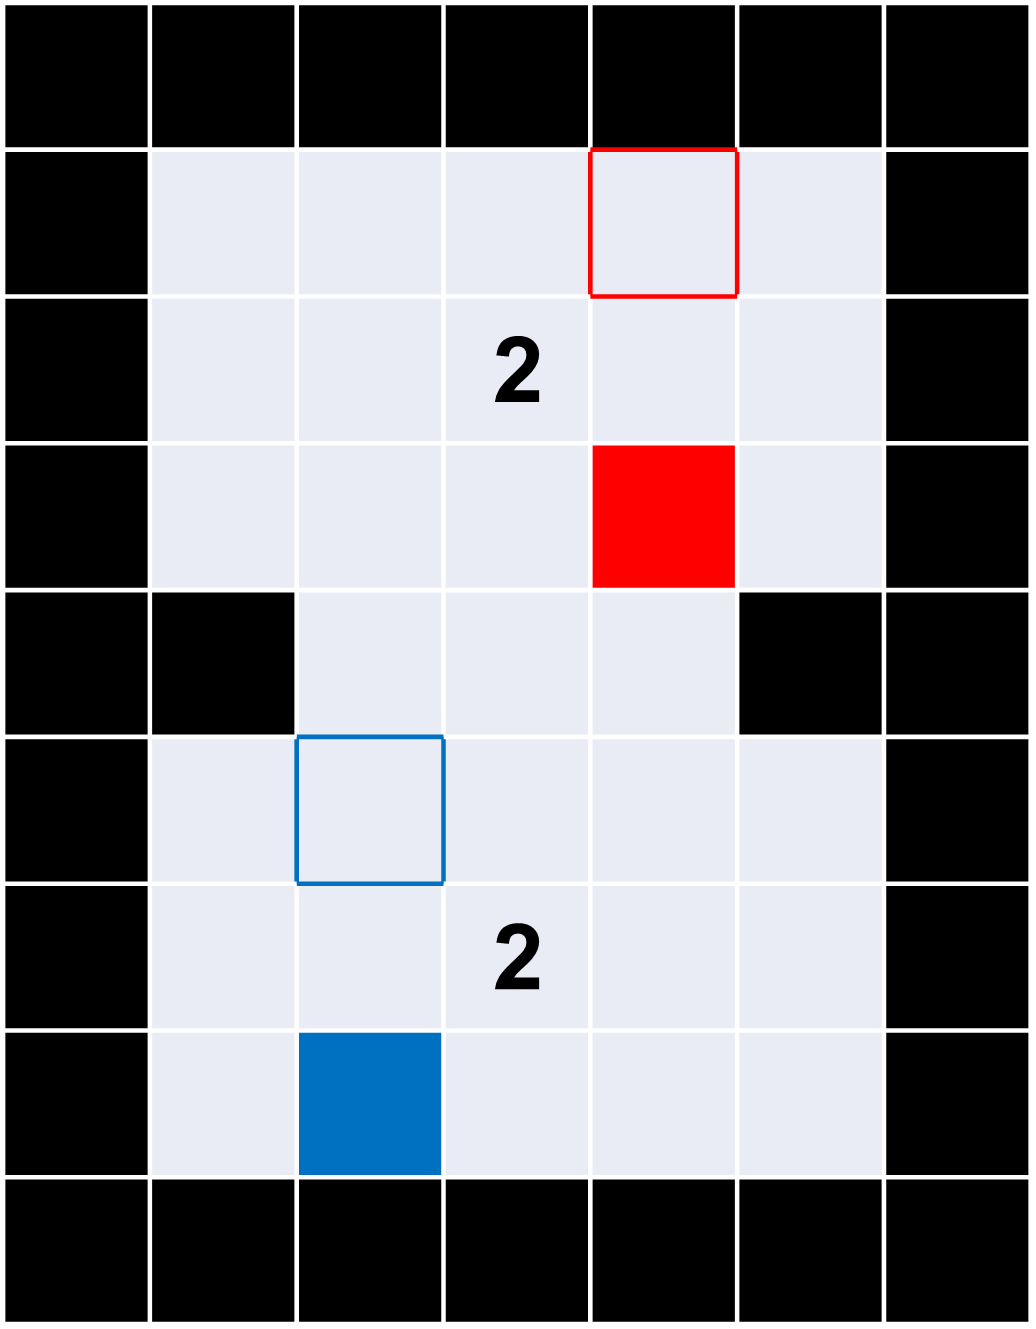
\includegraphics[width=0.1\textwidth]{Images/P1s.png}
        \label{subfig:s1}} 
    \subfigure[$S_2$]{
        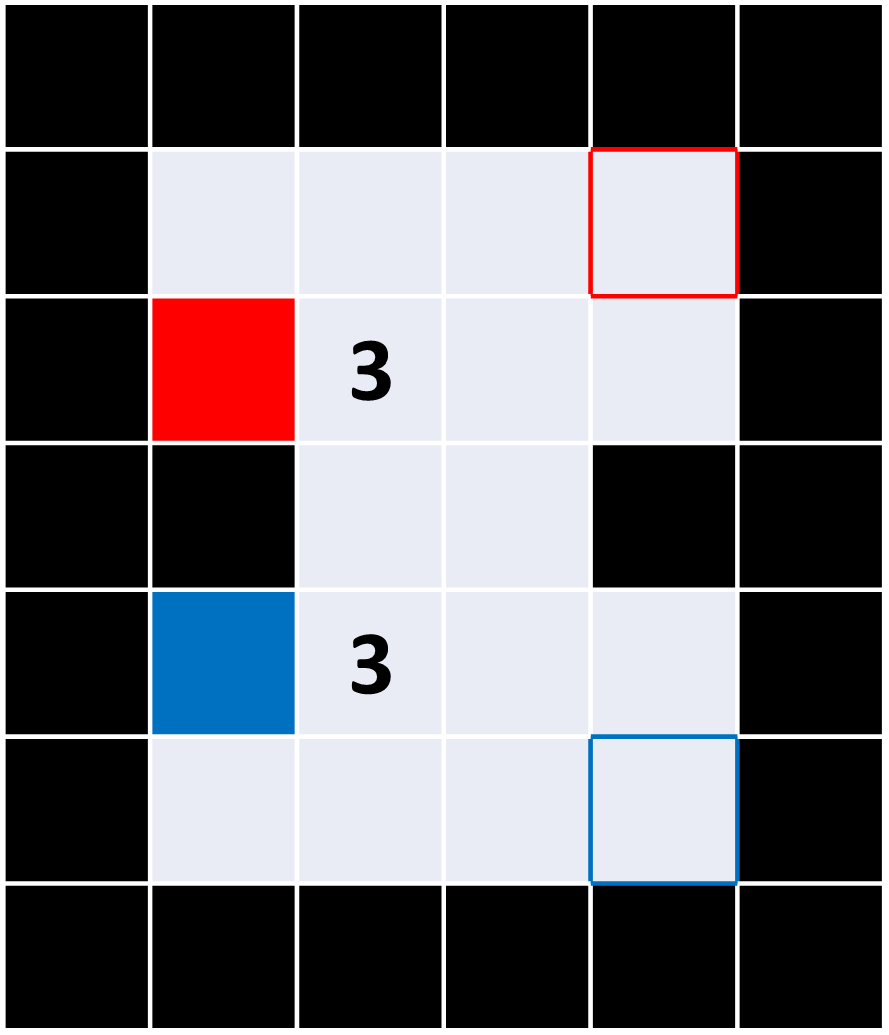
\includegraphics[width=0.11\textwidth]{Images/P2s.png}
        \label{subfig:s2}} 
    \subfigure[$S_3$]{
        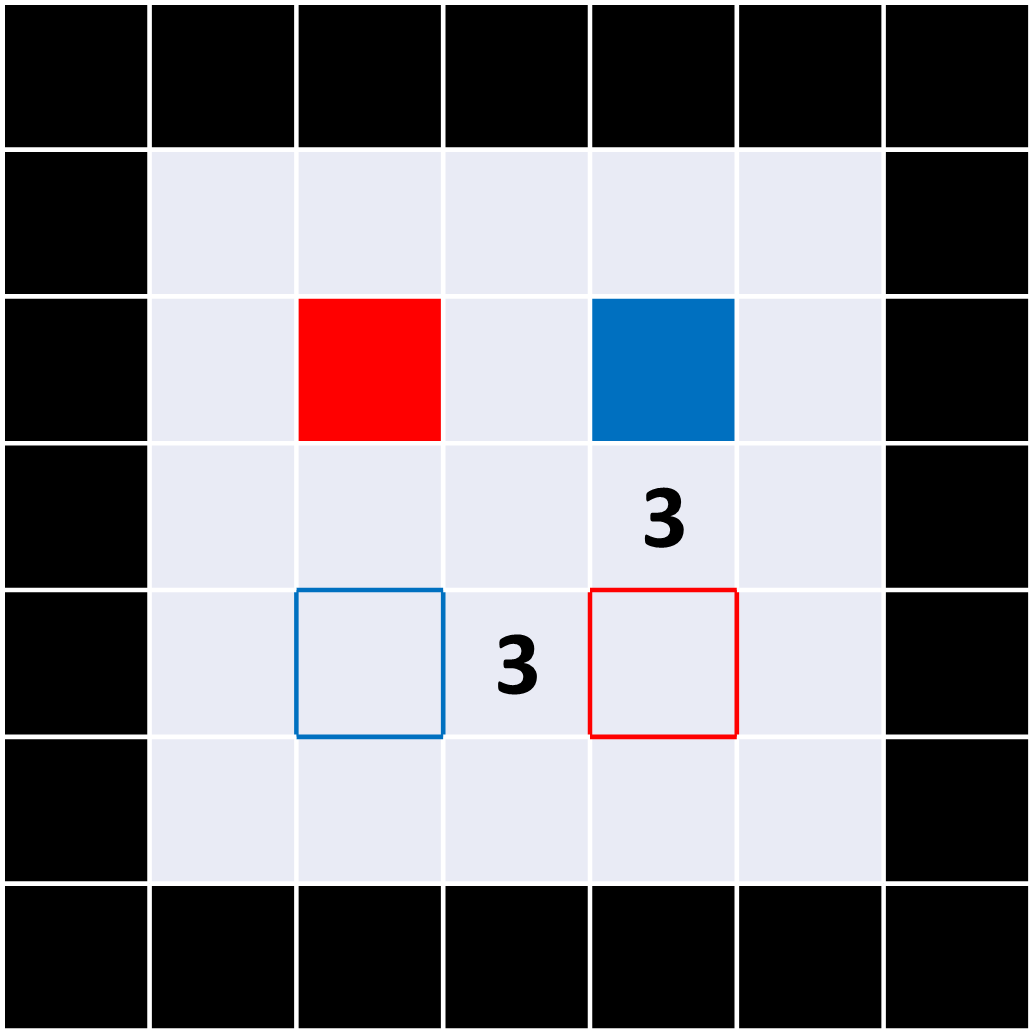
\includegraphics[width=0.13\textwidth]{Images/P3s.png}
        \label{subfig:s3}}
    \subfigure[$S_4$]{
        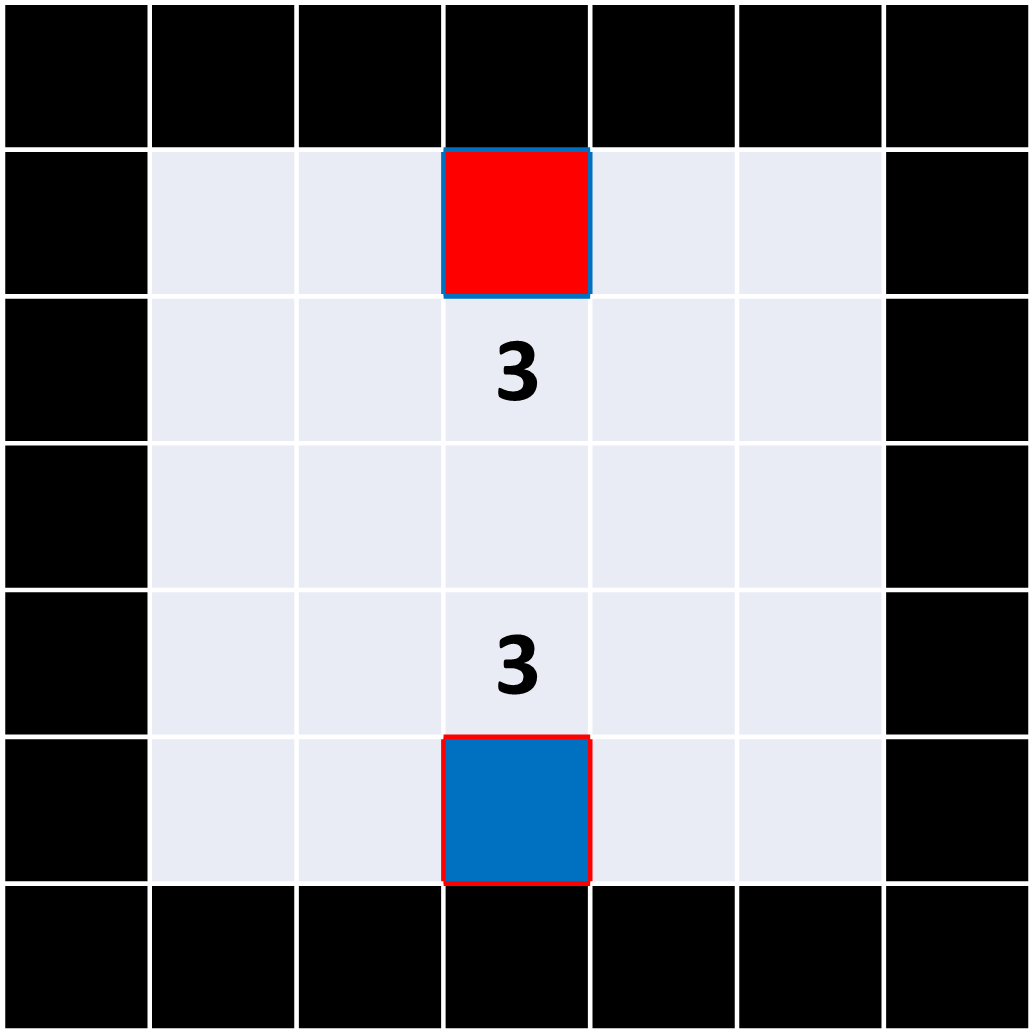
\includegraphics[width=0.13\textwidth]{Images/P4s.png}
        \label{subfig:$S_4$}}
    \caption{The small Grid SMAPF-PO problems in our benchmarks.}
    \label{fig:small-multi-problems}        
\end{figure}

\begin{figure}
\subfigure[$M_1$]{
        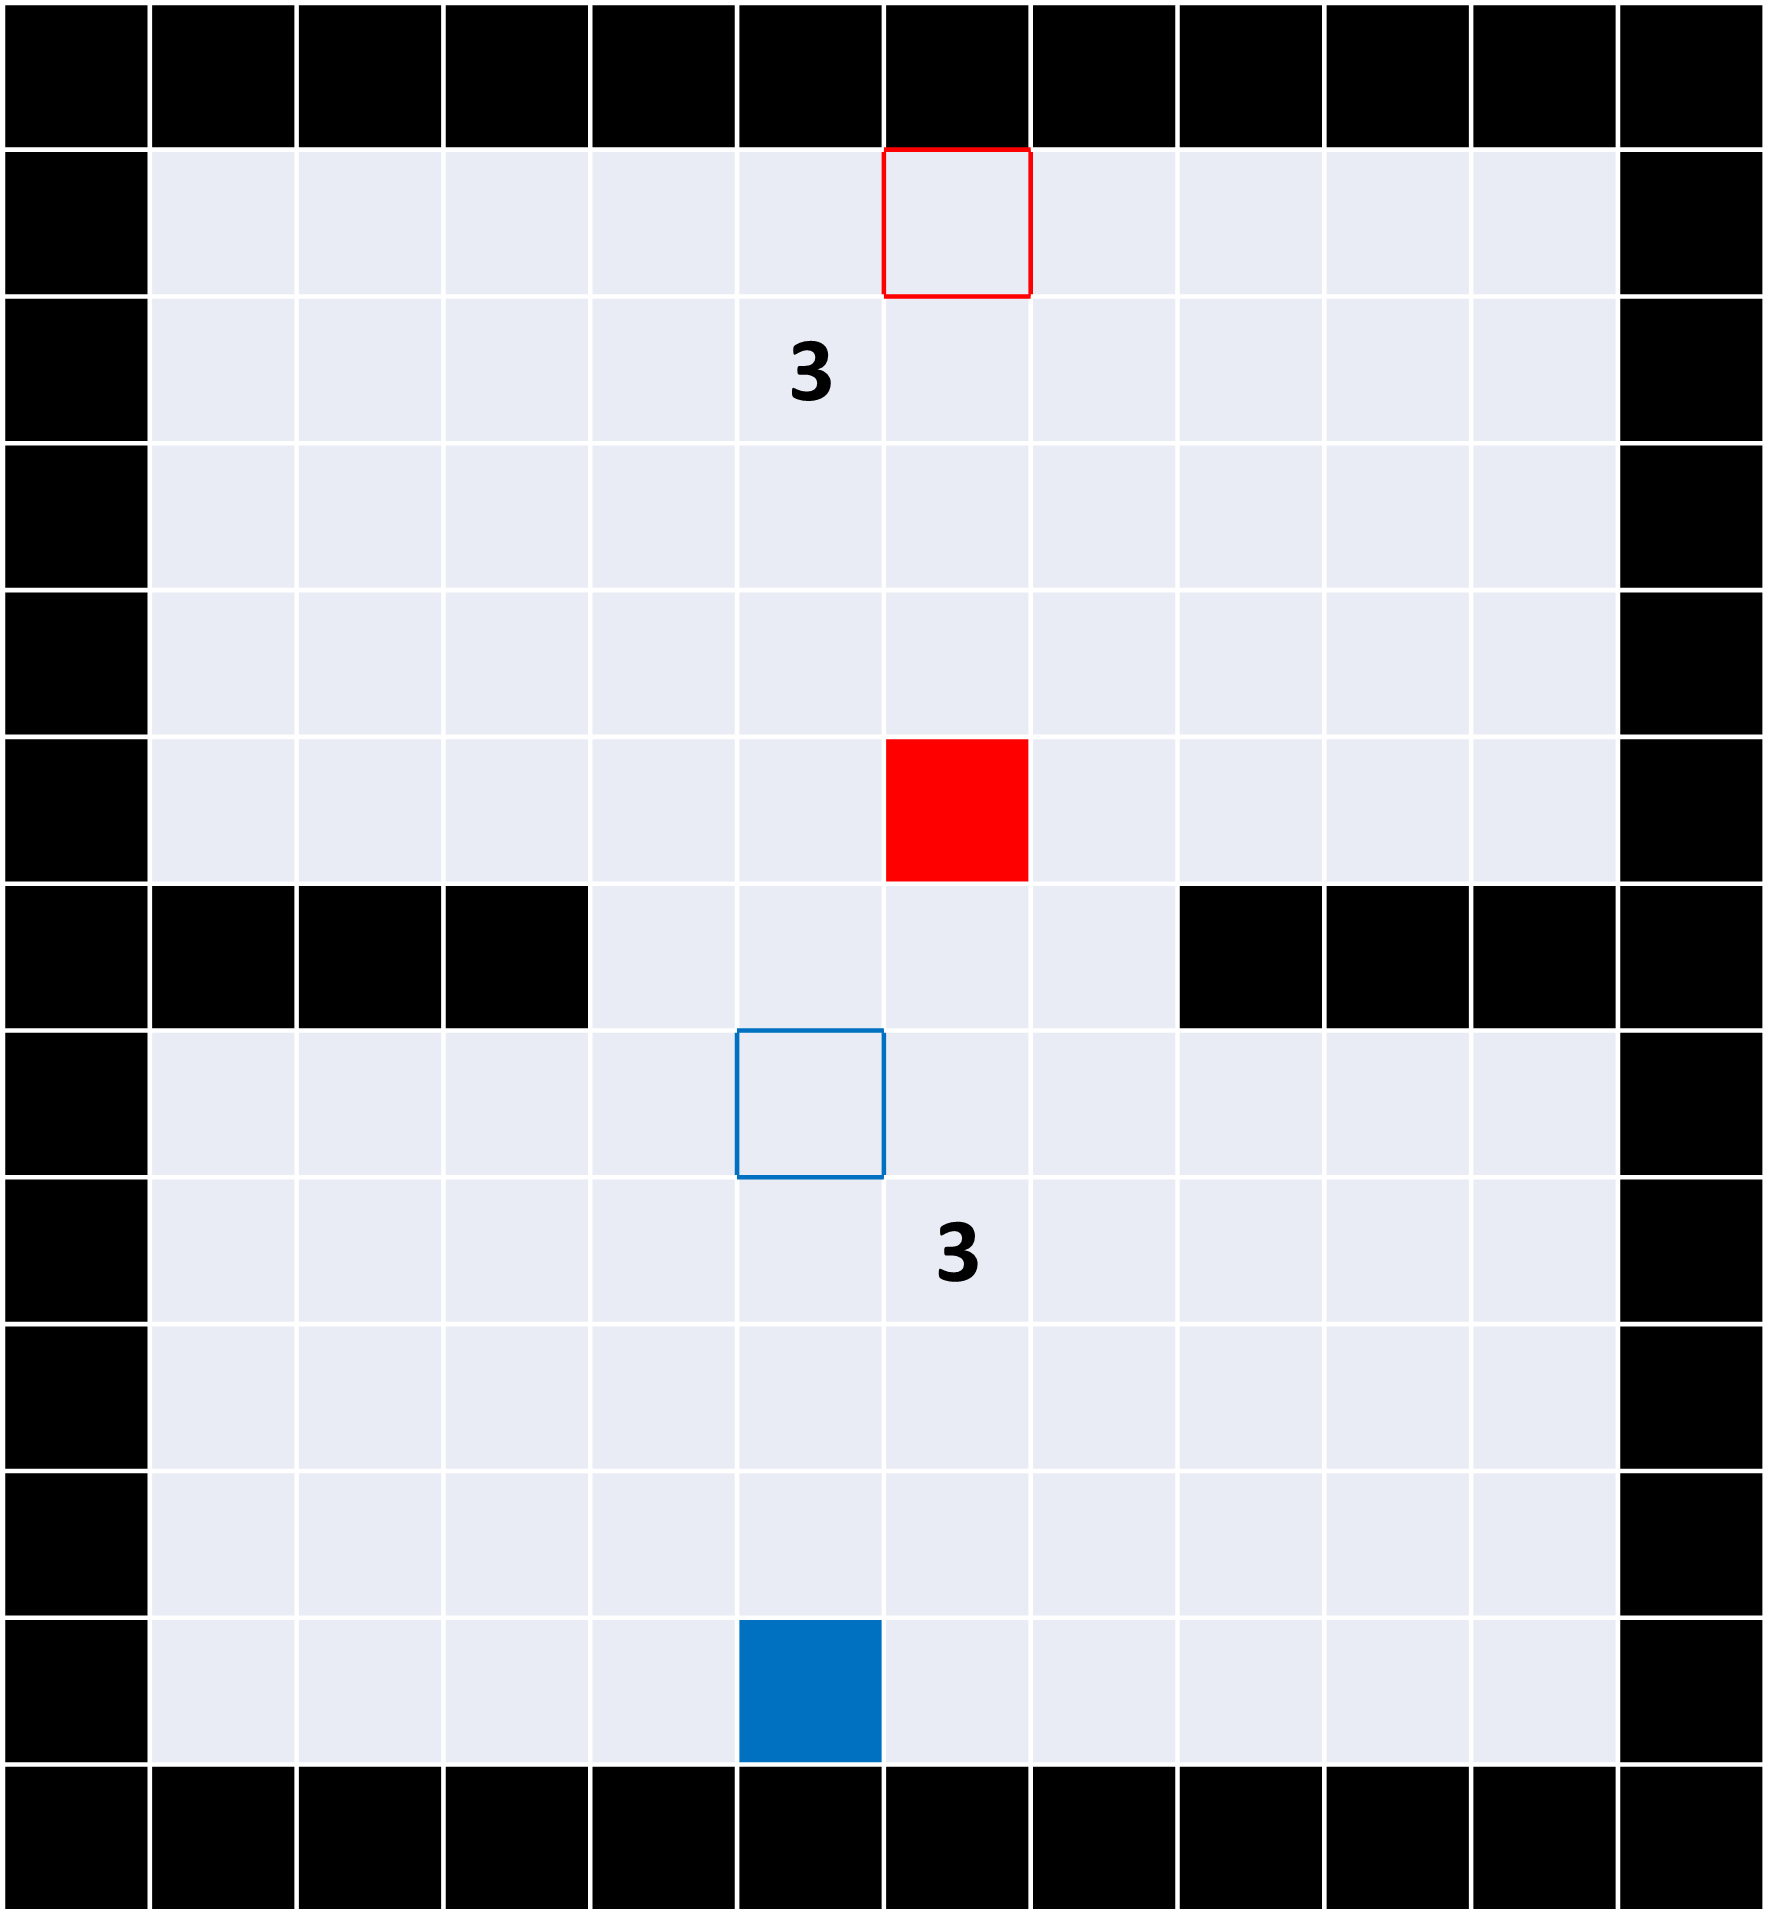
\includegraphics[width=0.12\textwidth]{Images/P1.png}
        \label{subfig:m1}} 
    \subfigure[$M_2$]{
        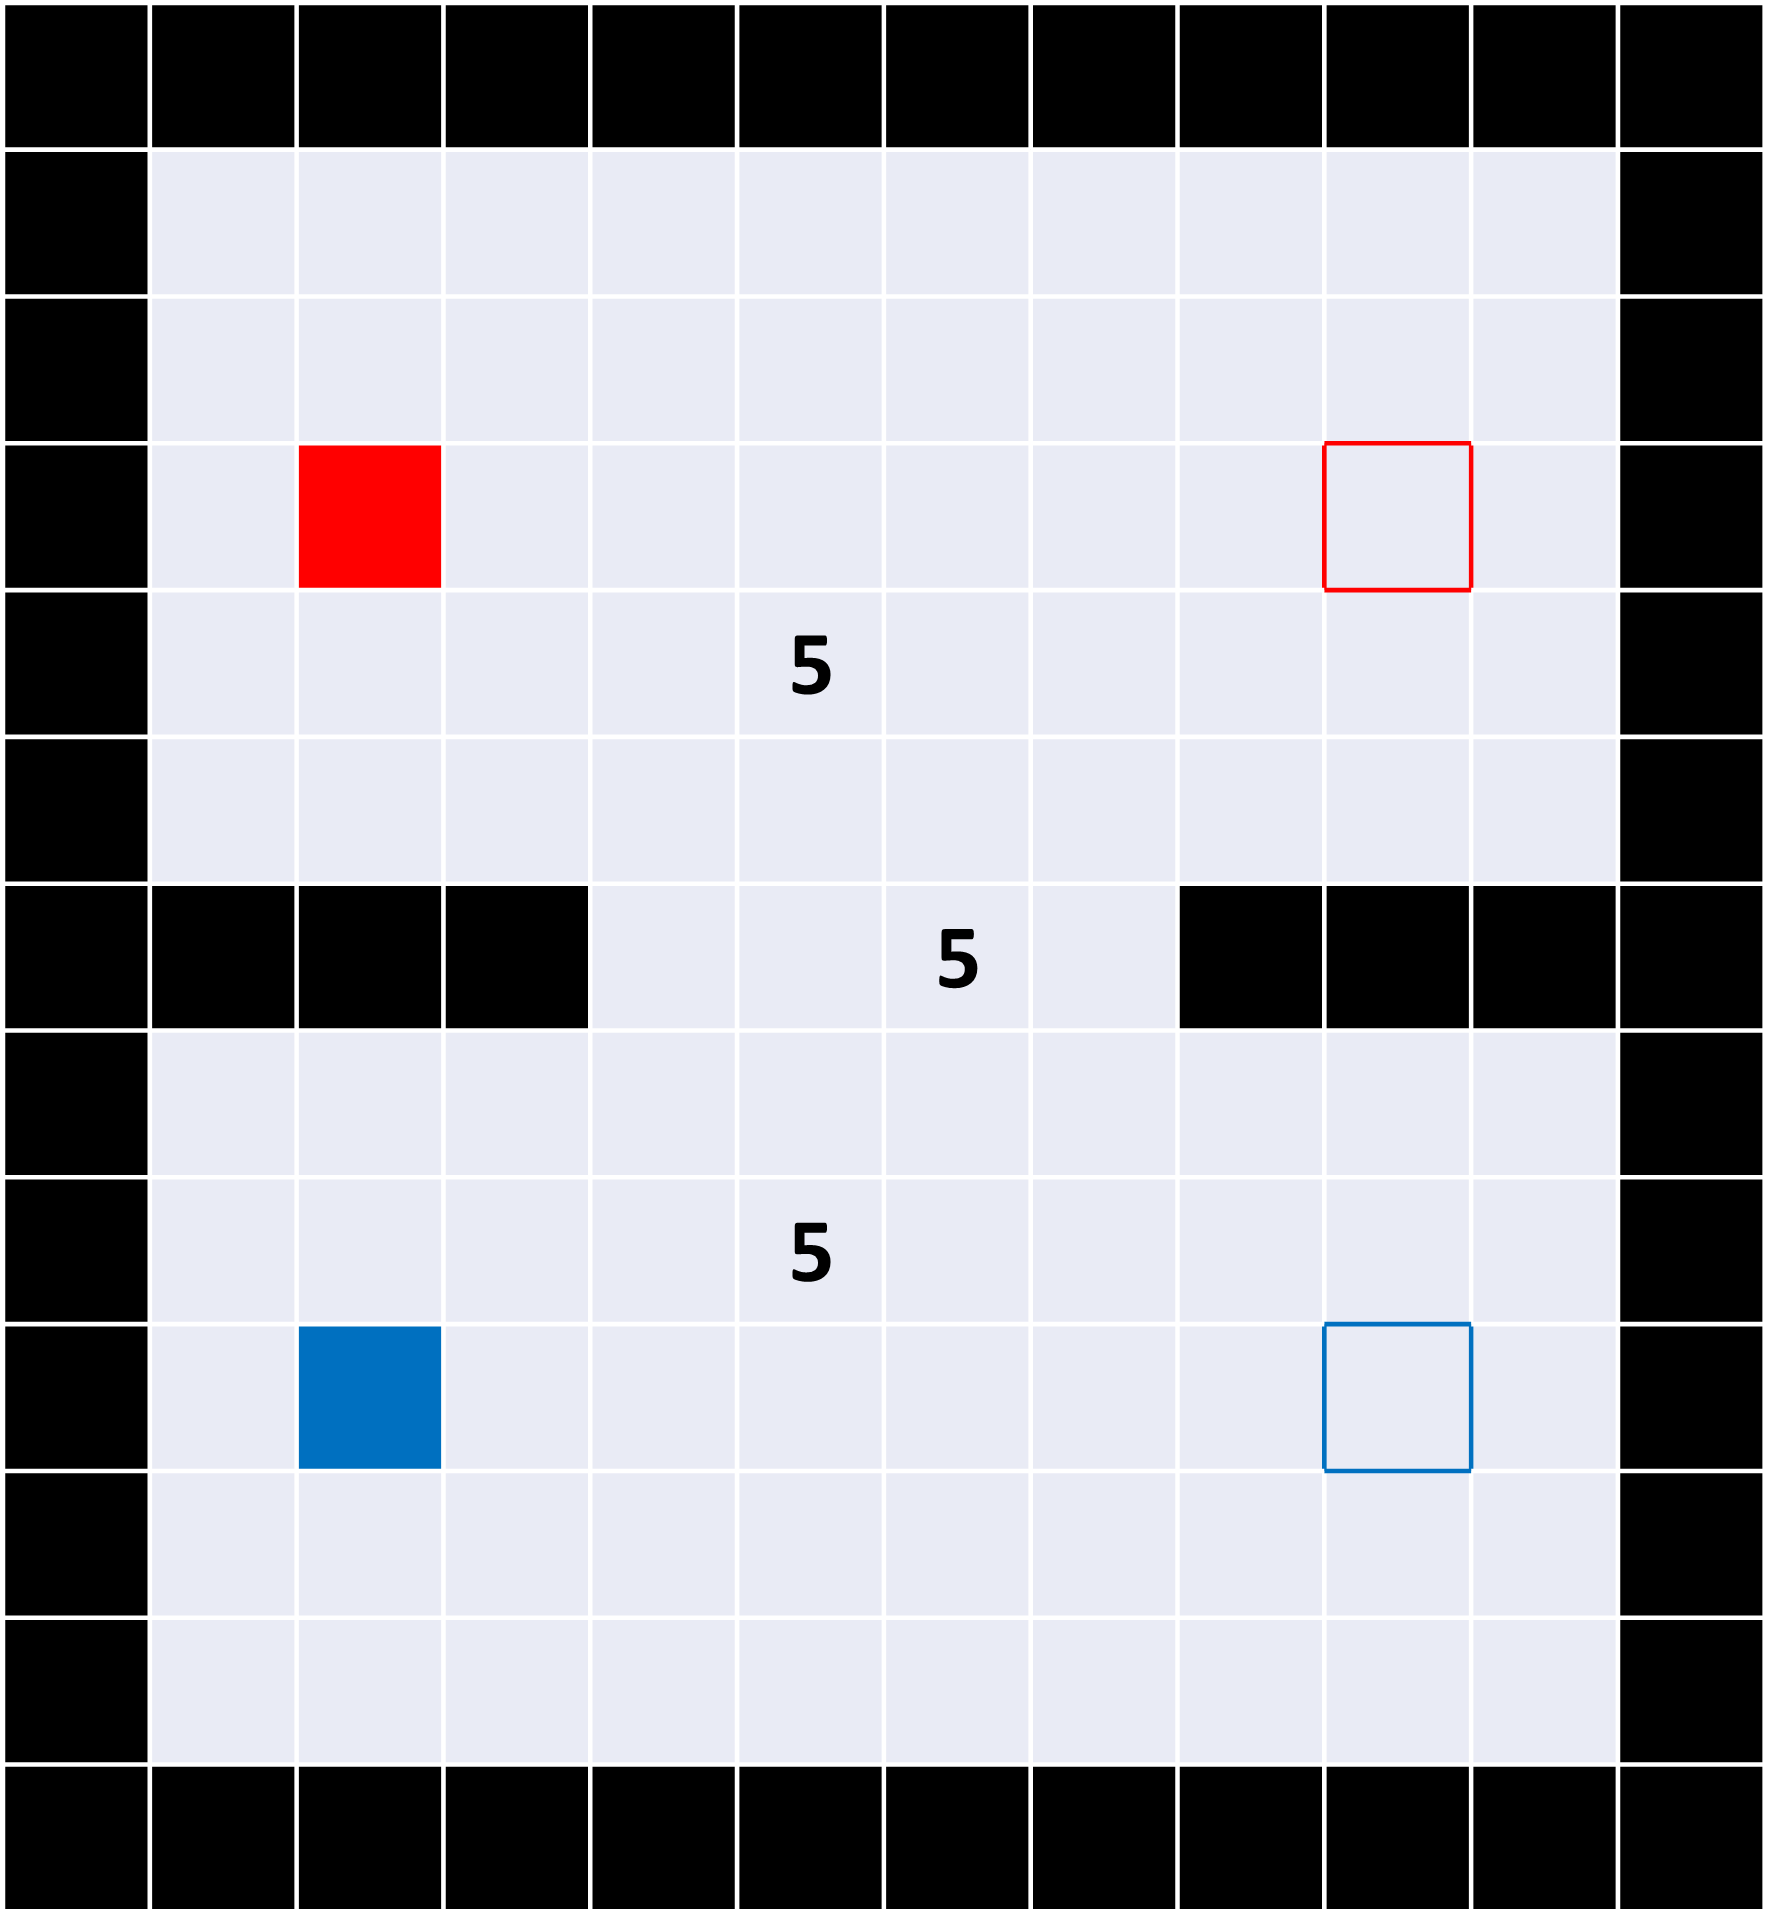
\includegraphics[width=0.12\textwidth]{Images/P2.png}
        \label{subfig:m2}} 
    \subfigure[$M_3$]{
        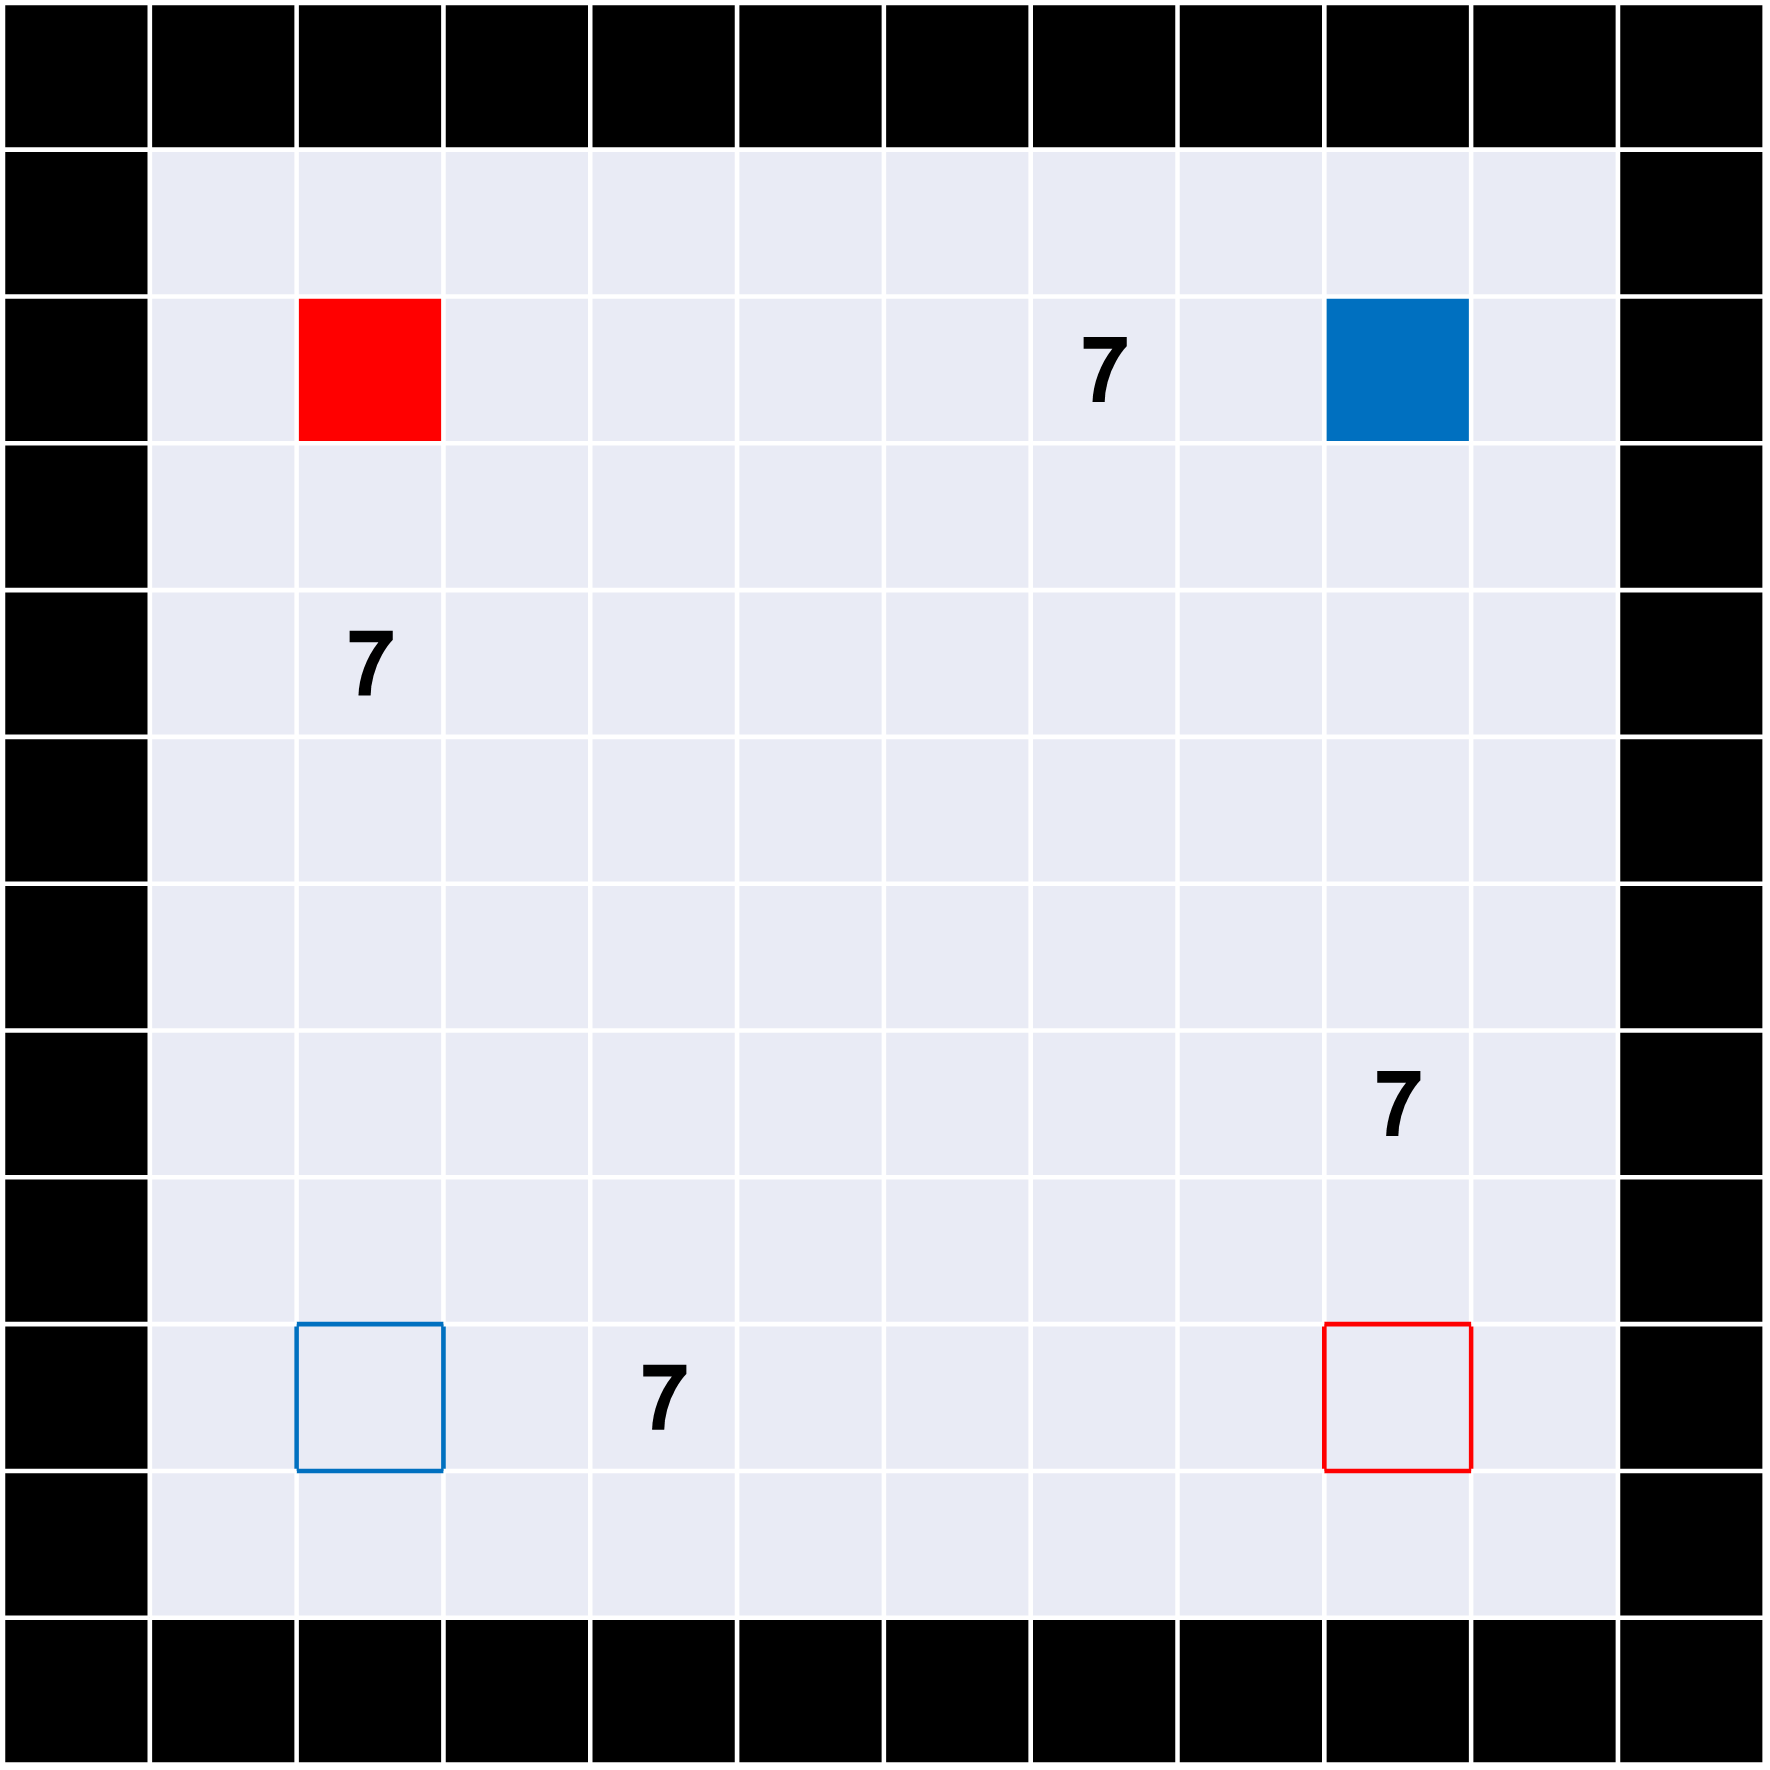
\includegraphics[width=0.13\textwidth]{Images/P3.png}
        \label{subfig:m3}}
    \subfigure[$M_4$]{
        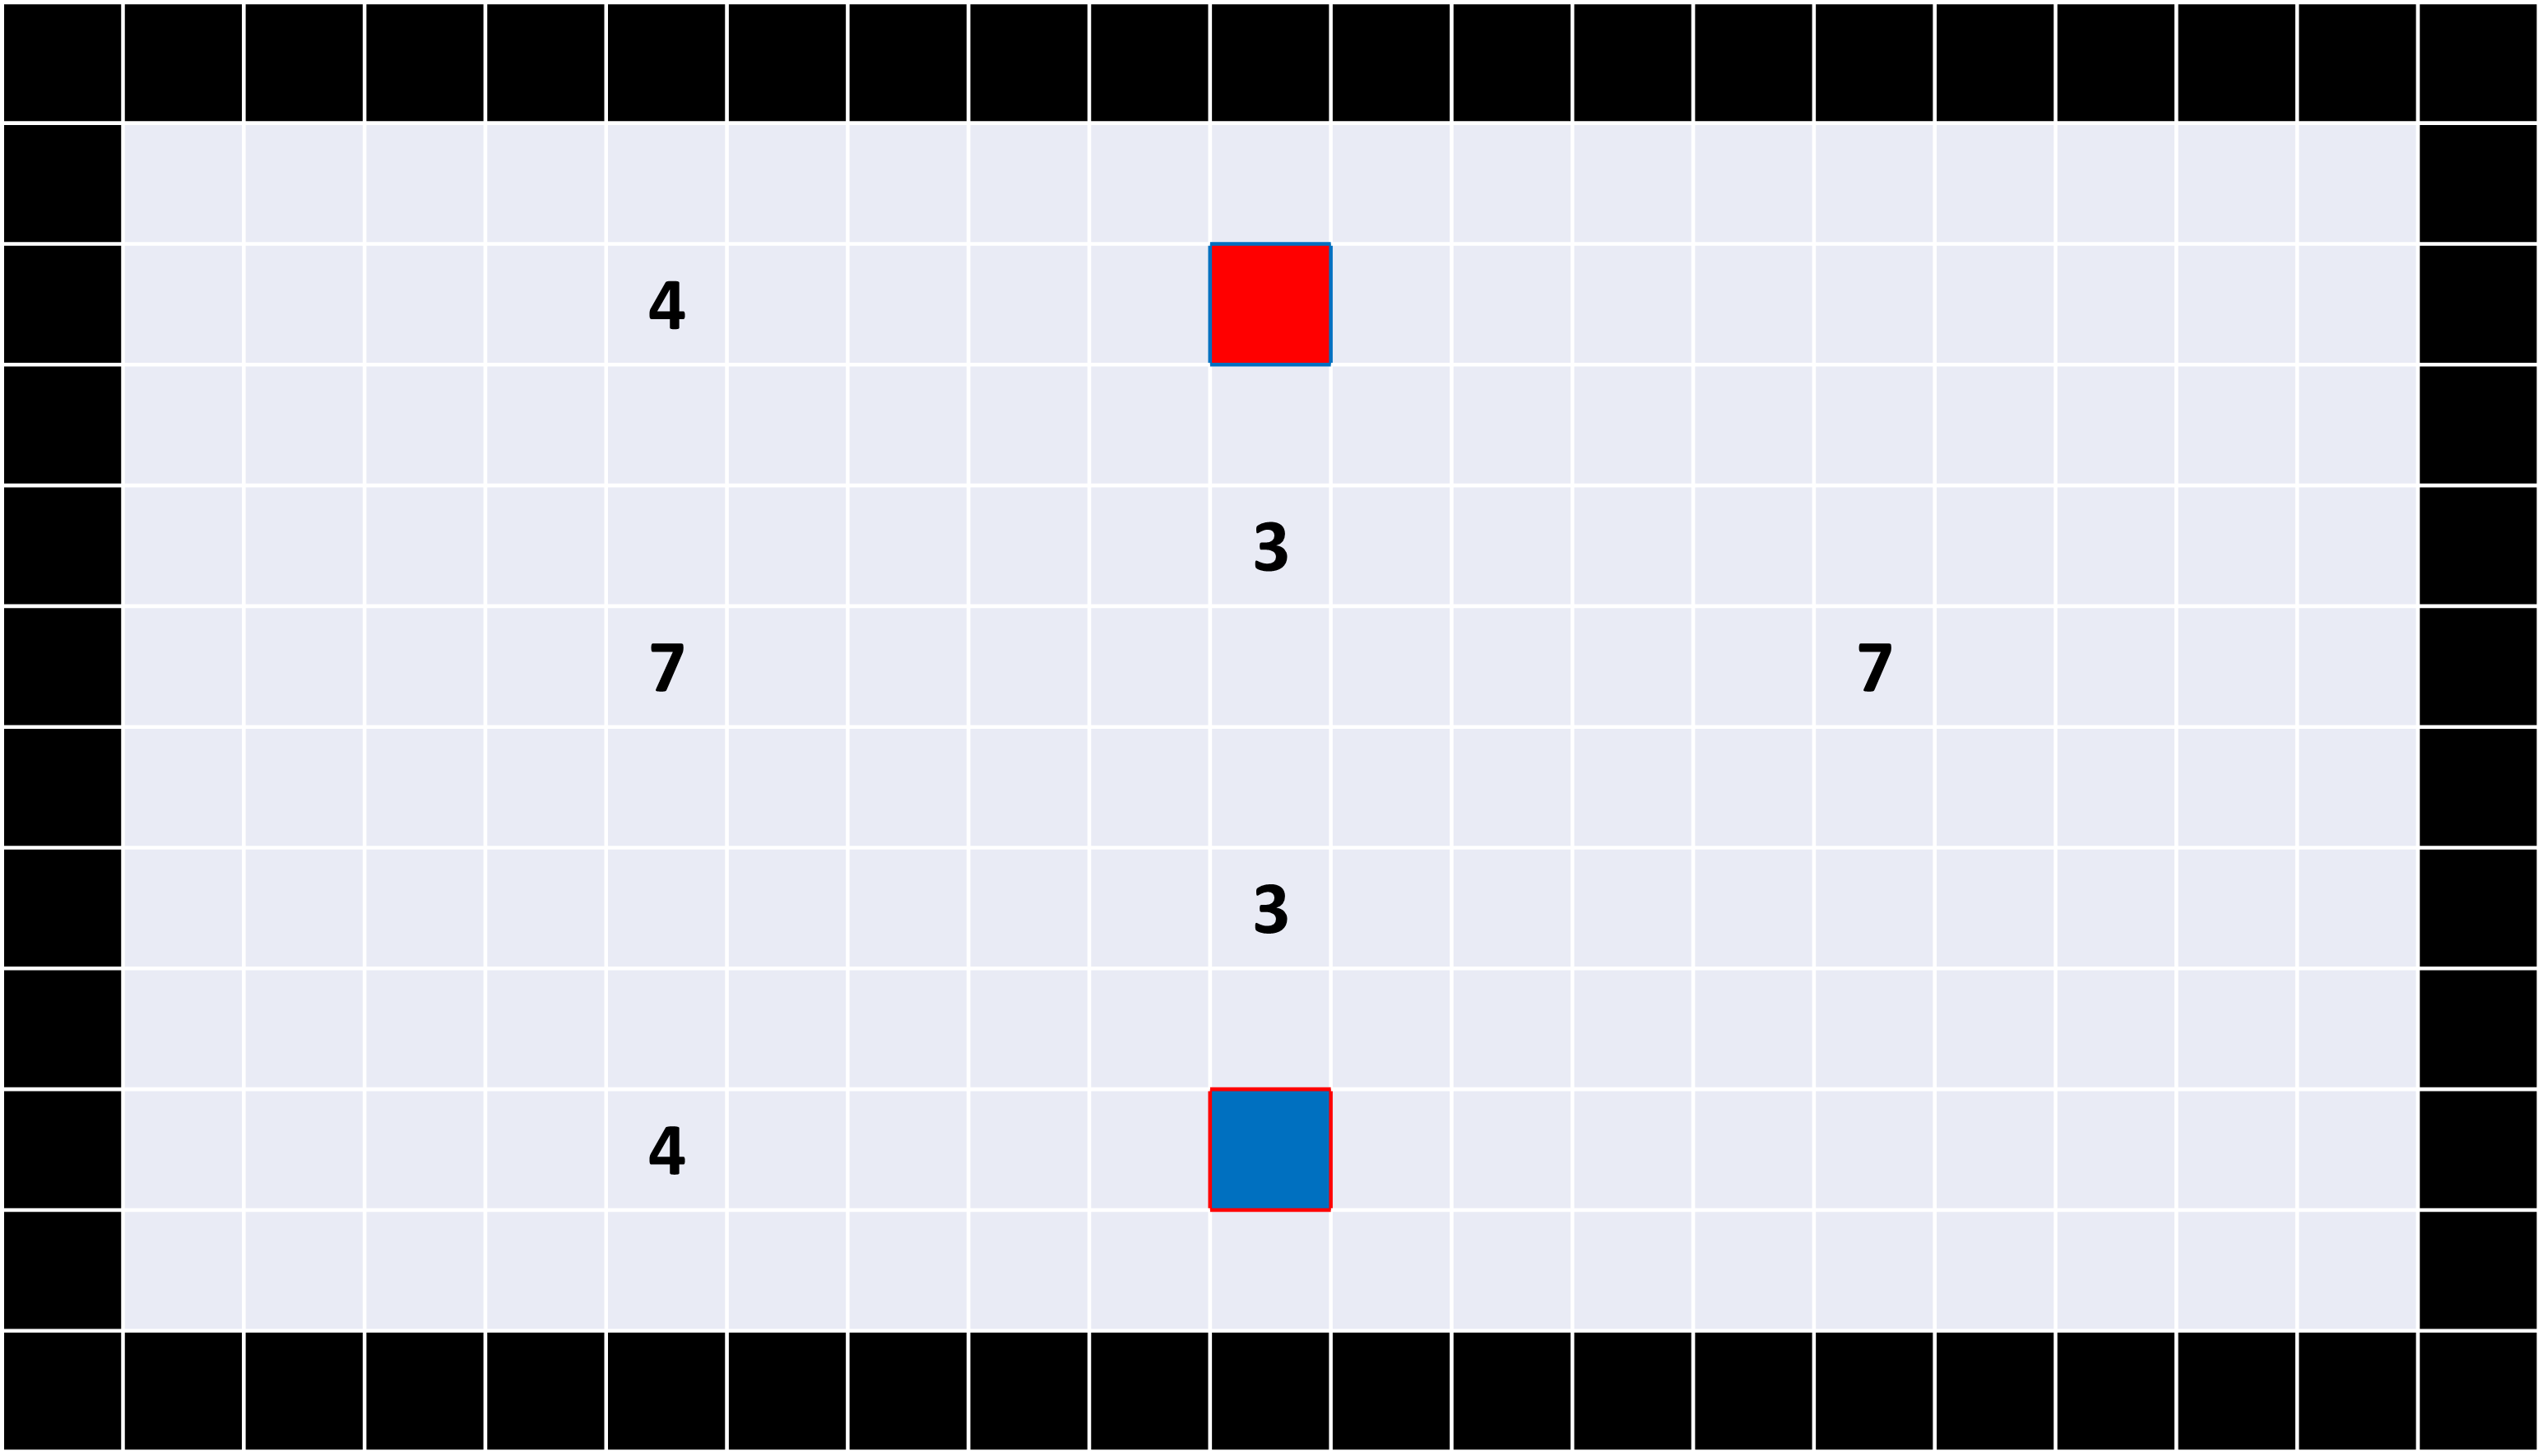
\includegraphics[width=0.245\textwidth]{Images/P4.png}
        \label{subfig:m4}}
    \subfigure[$M_5$]{
        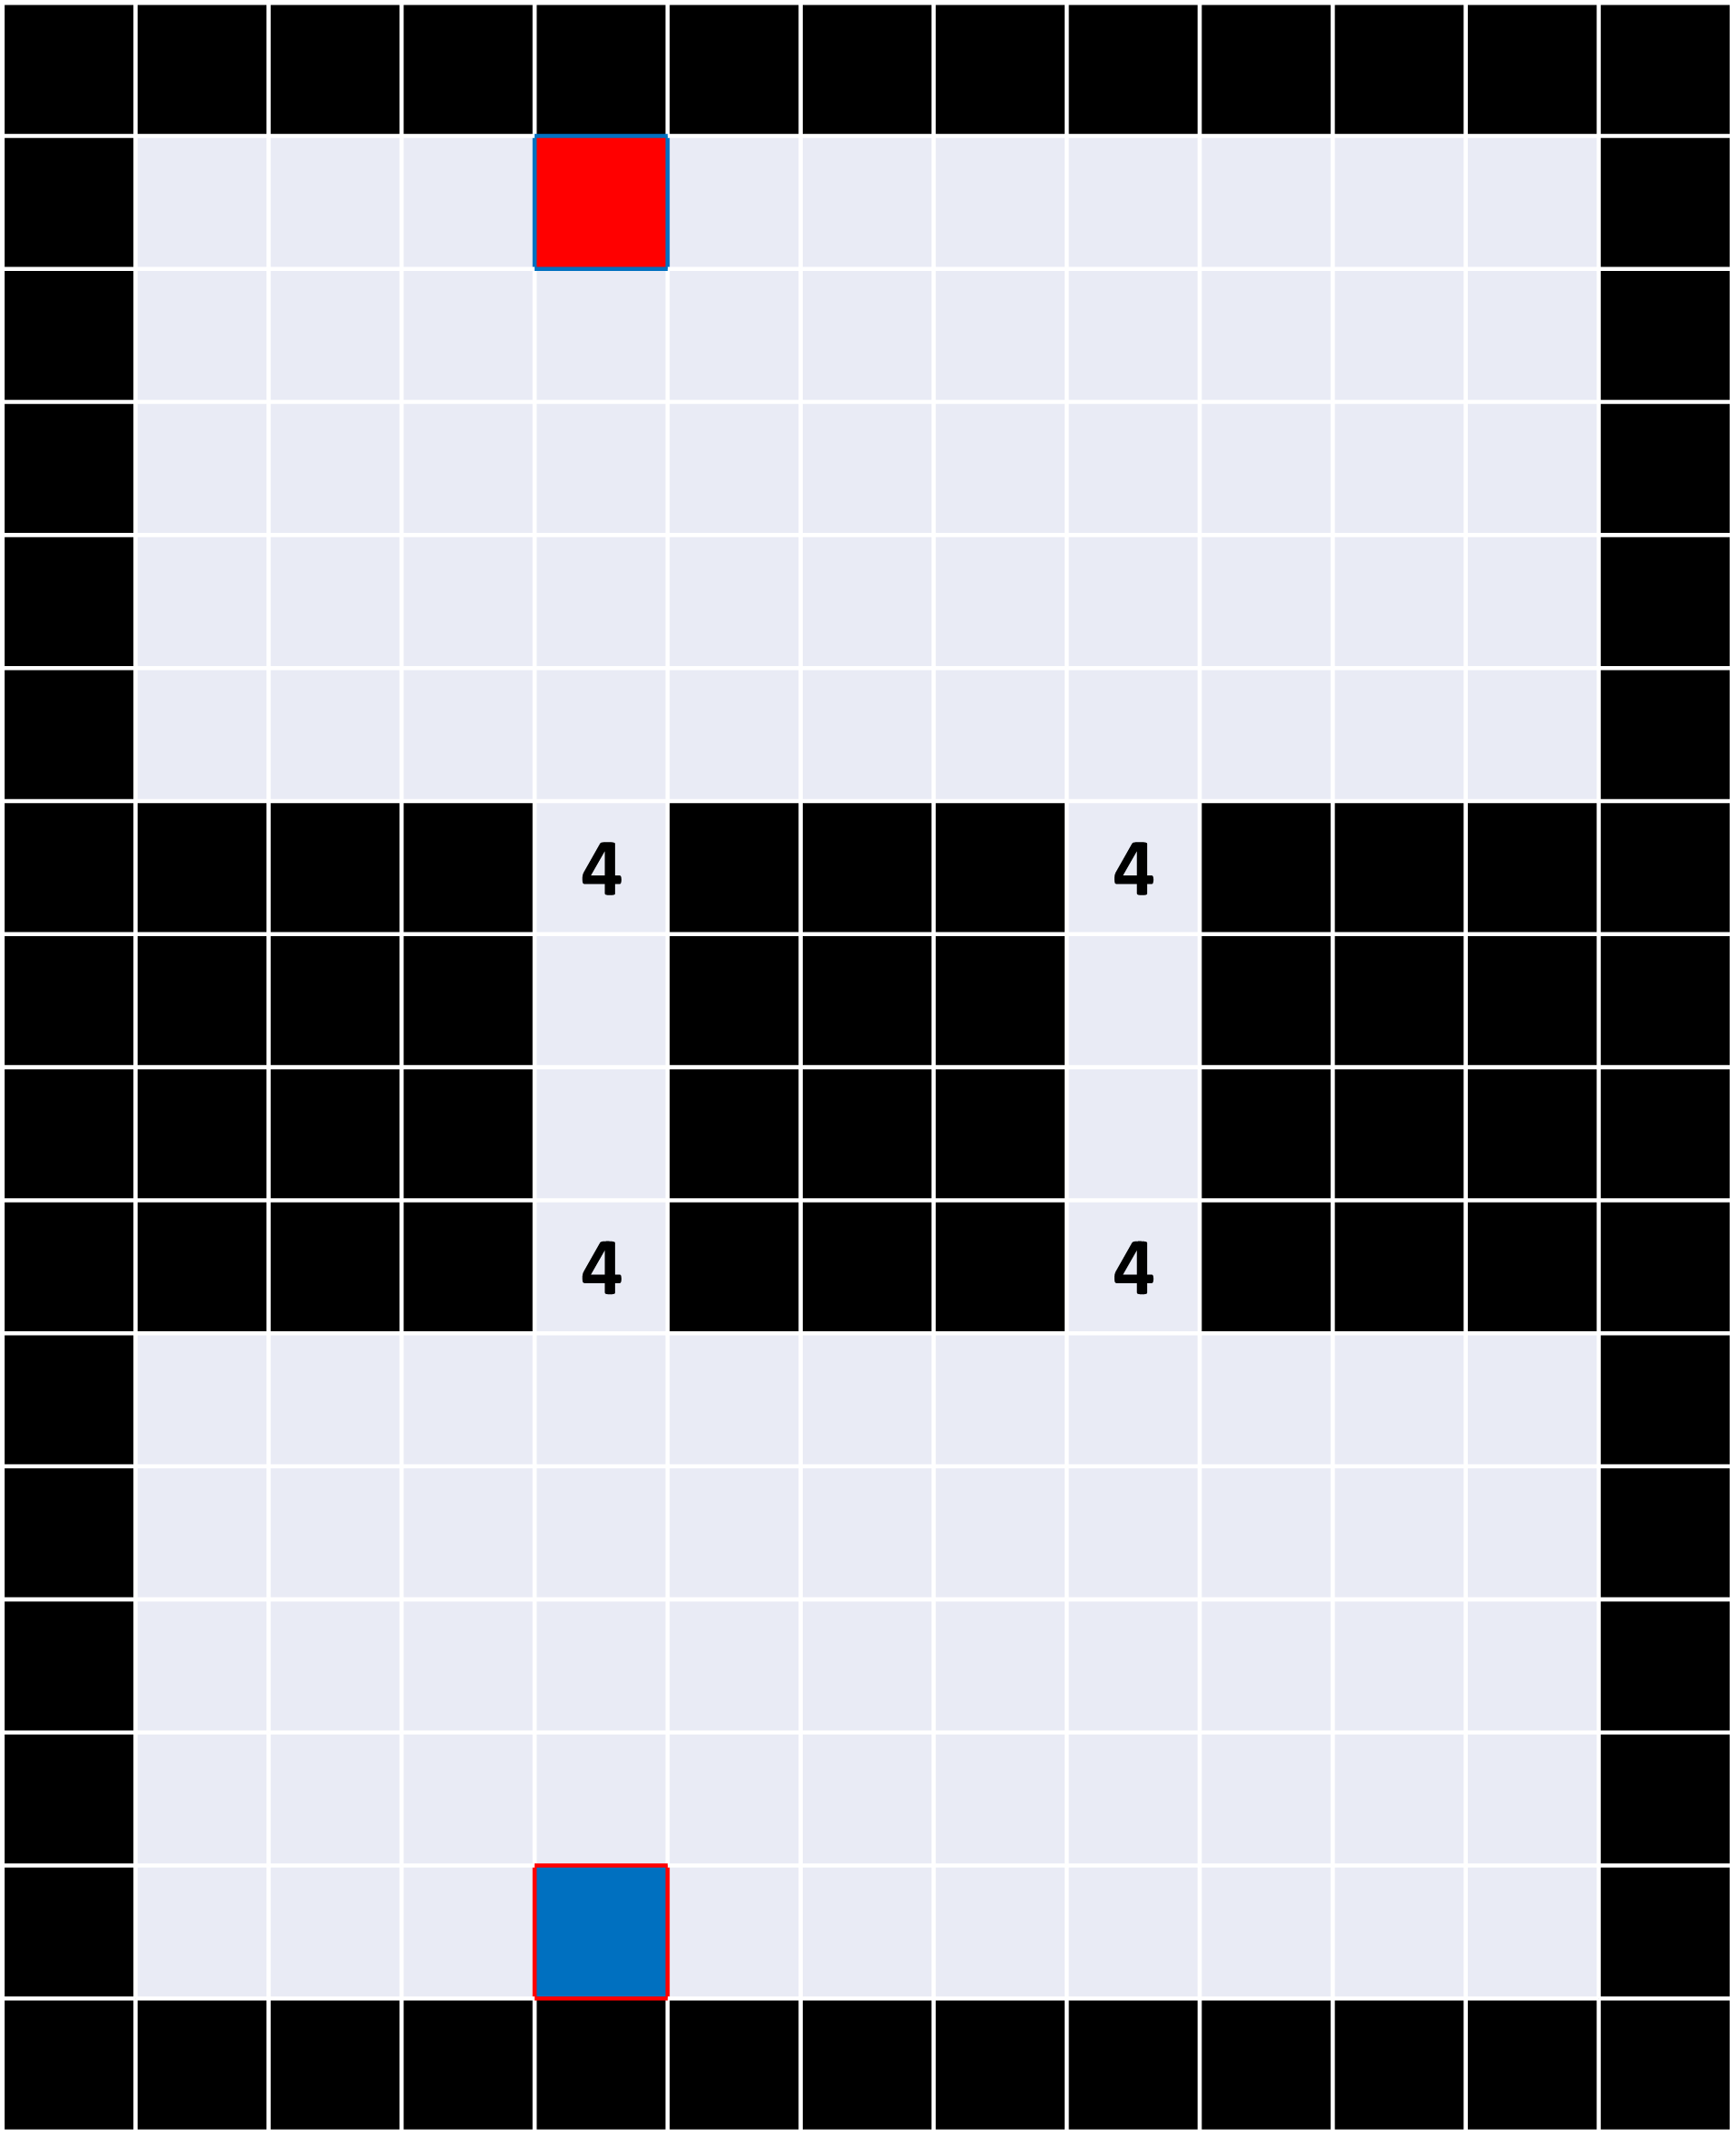
\includegraphics[width=0.115\textwidth]{Images/P5.png}
        \label{subfig:m5}}
    \caption{The medium-sized Grid SMAPF-PO problems in our benchmarks.}
    \label{fig:medium-multi-problems}                
\end{figure}

\begin{figure}
     \subfigure[$L_1$]{
        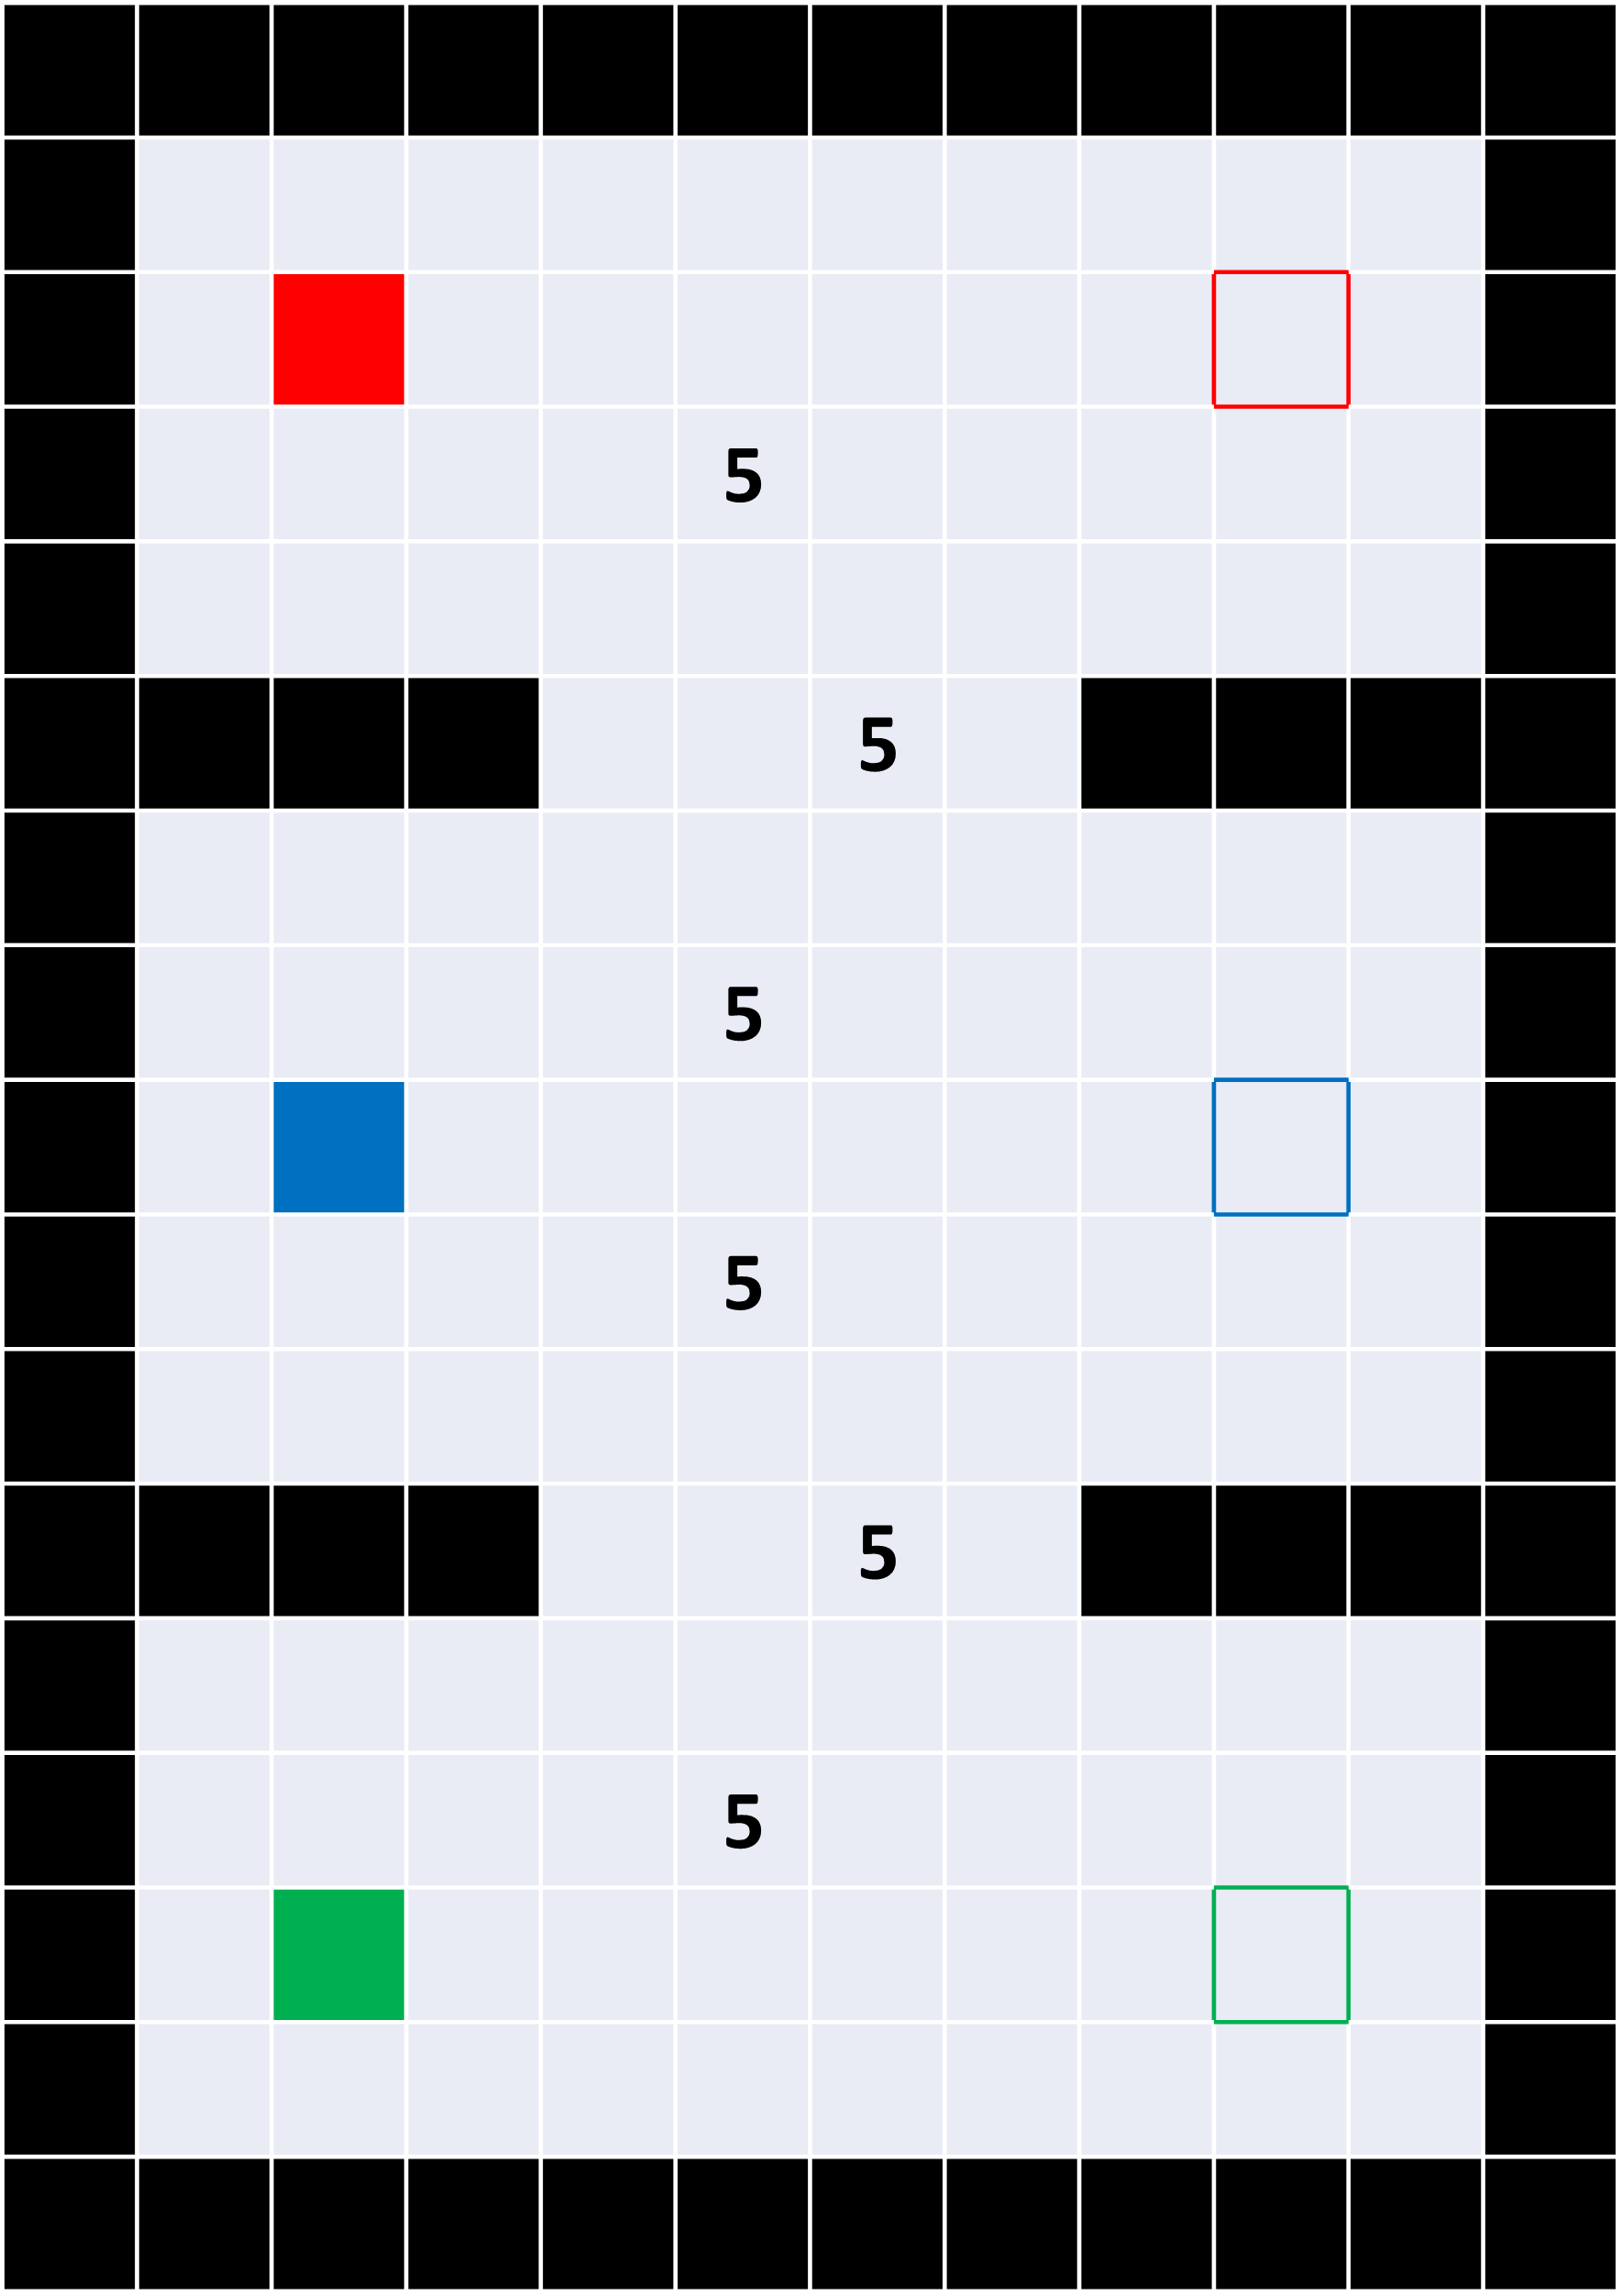
\includegraphics[width=0.1\textwidth]{Images/P2-3a.png}
        \label{subfig:l1}}
    \subfigure[$L_2$]{
        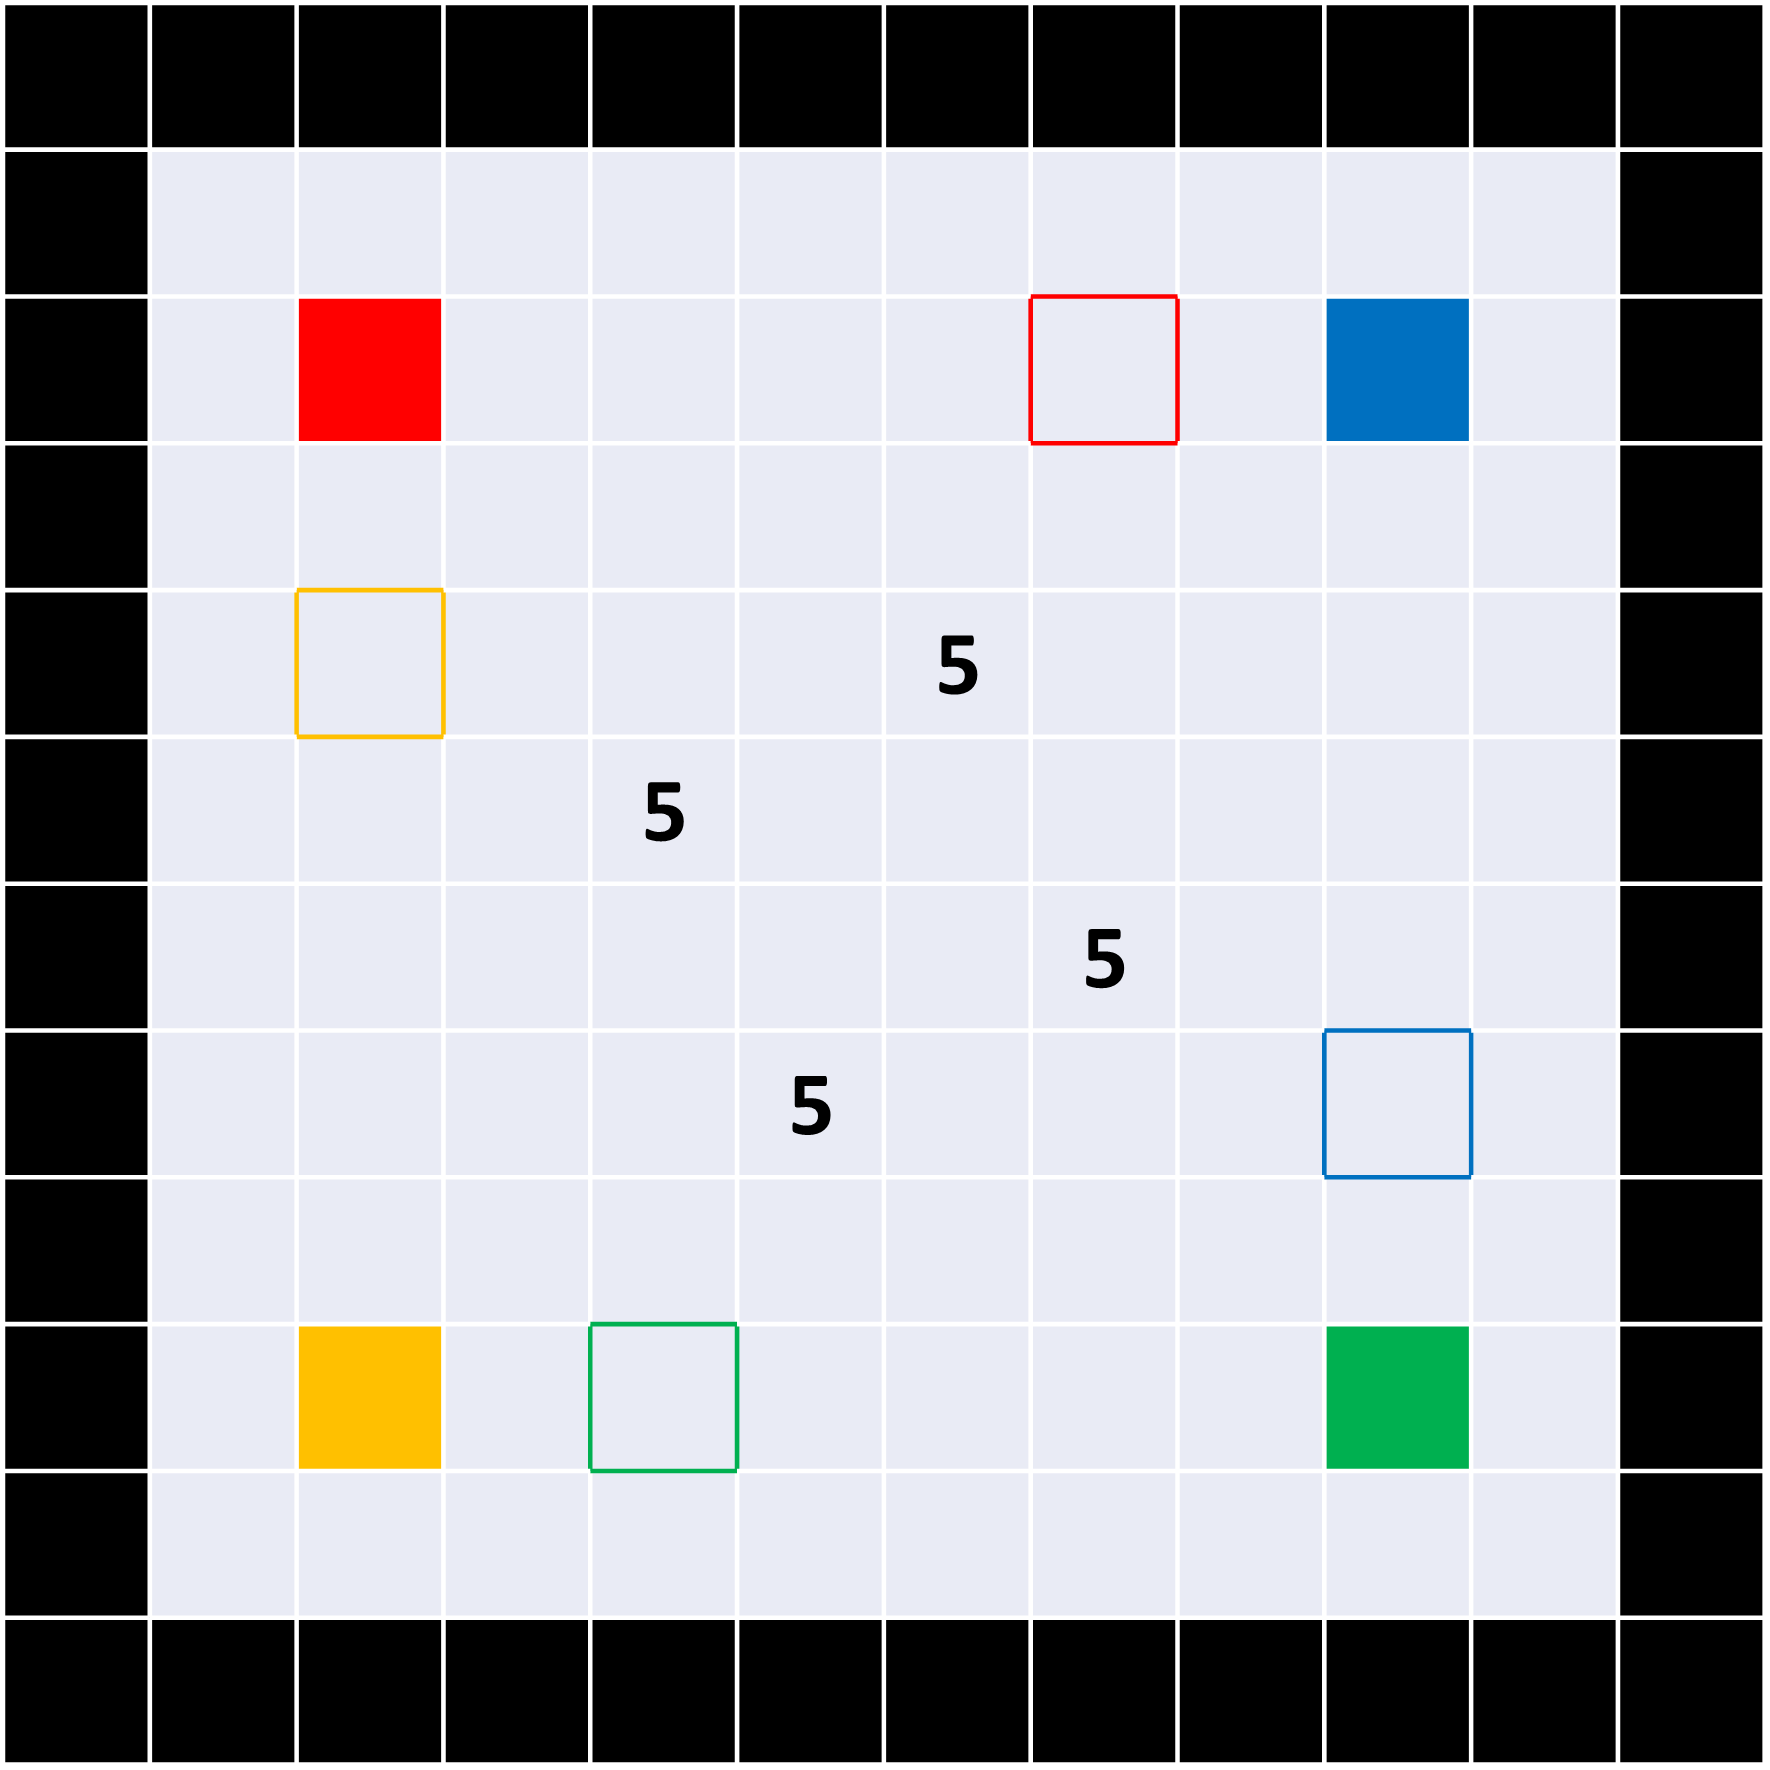
\includegraphics[width=0.1425\textwidth]{Images/P3-4a.png}
        \label{subfig:l2}}
    \subfigure[$L_3$]{
        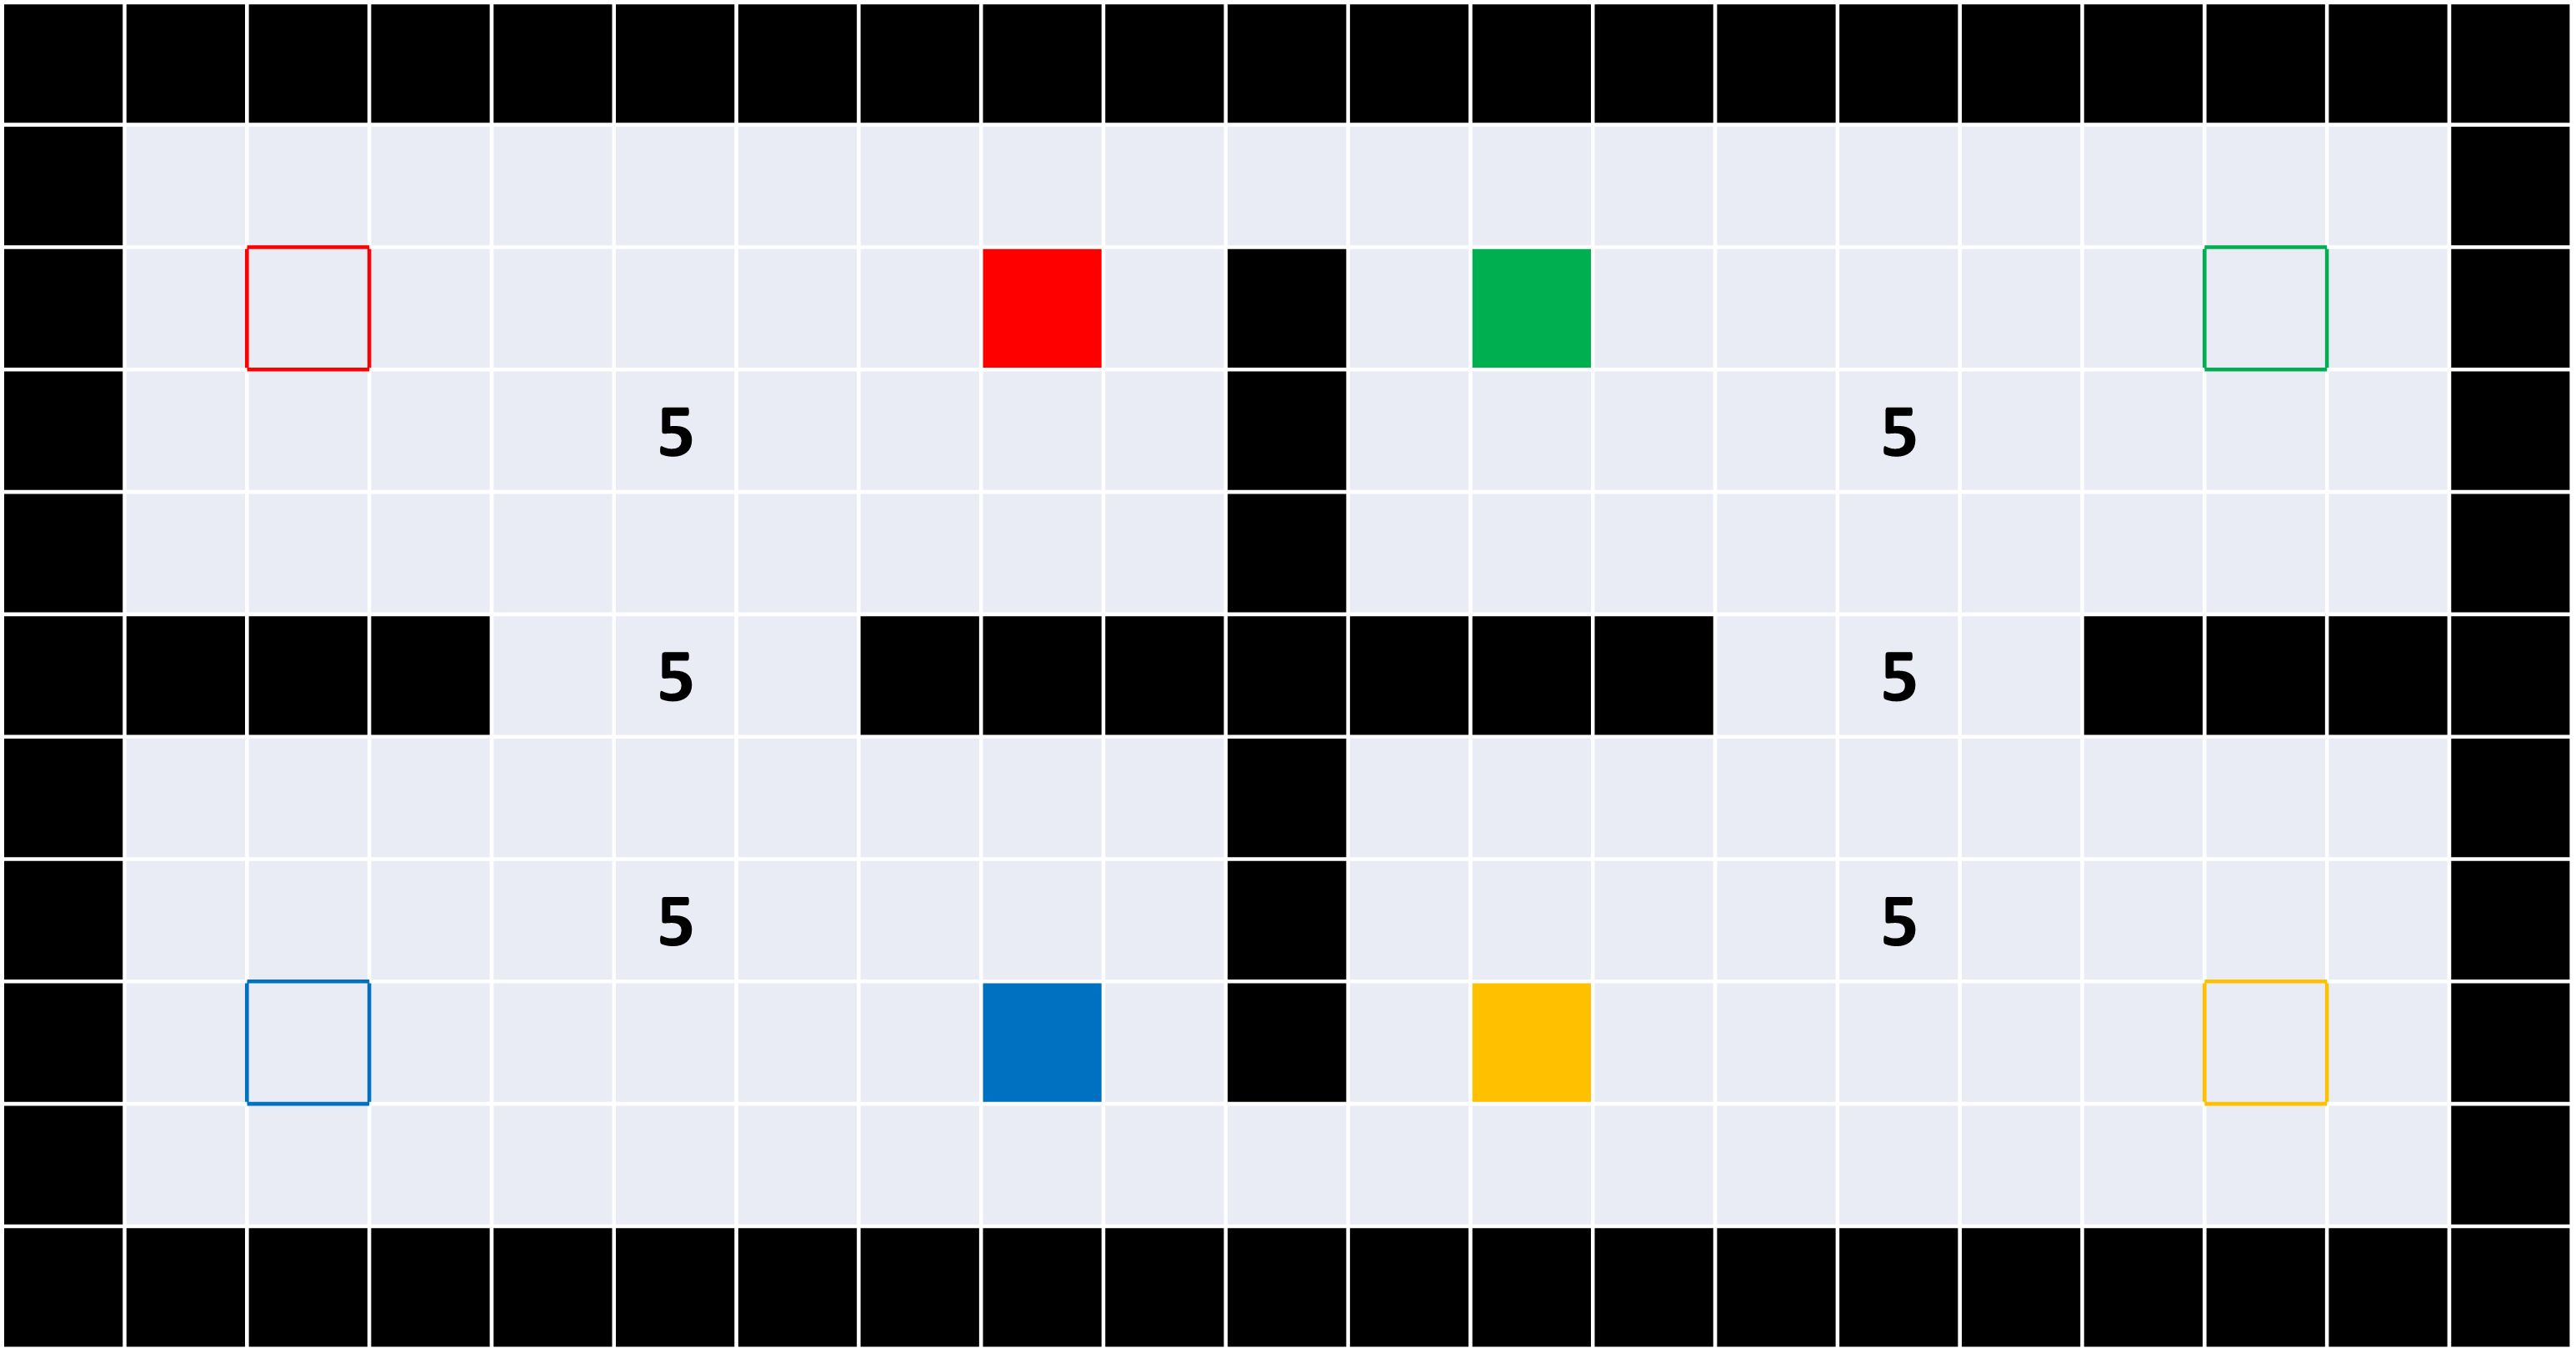
\includegraphics[width=0.27\textwidth]{Images/P2-4a.png}
        \label{subfig:l3}} 
    \caption{The large Grid SMAPF-PO problems in our benchmarks.}
    \label{fig:large-multi-problems}              
\end{figure}

% \begin{figure*}[b!]
% %    \caption{2 agents' smaller benchmarks, used to compare our algorithm to a joint offline version.}
% %    \label{fig:small-problems}
% \subfigure[$M_1$]{
%         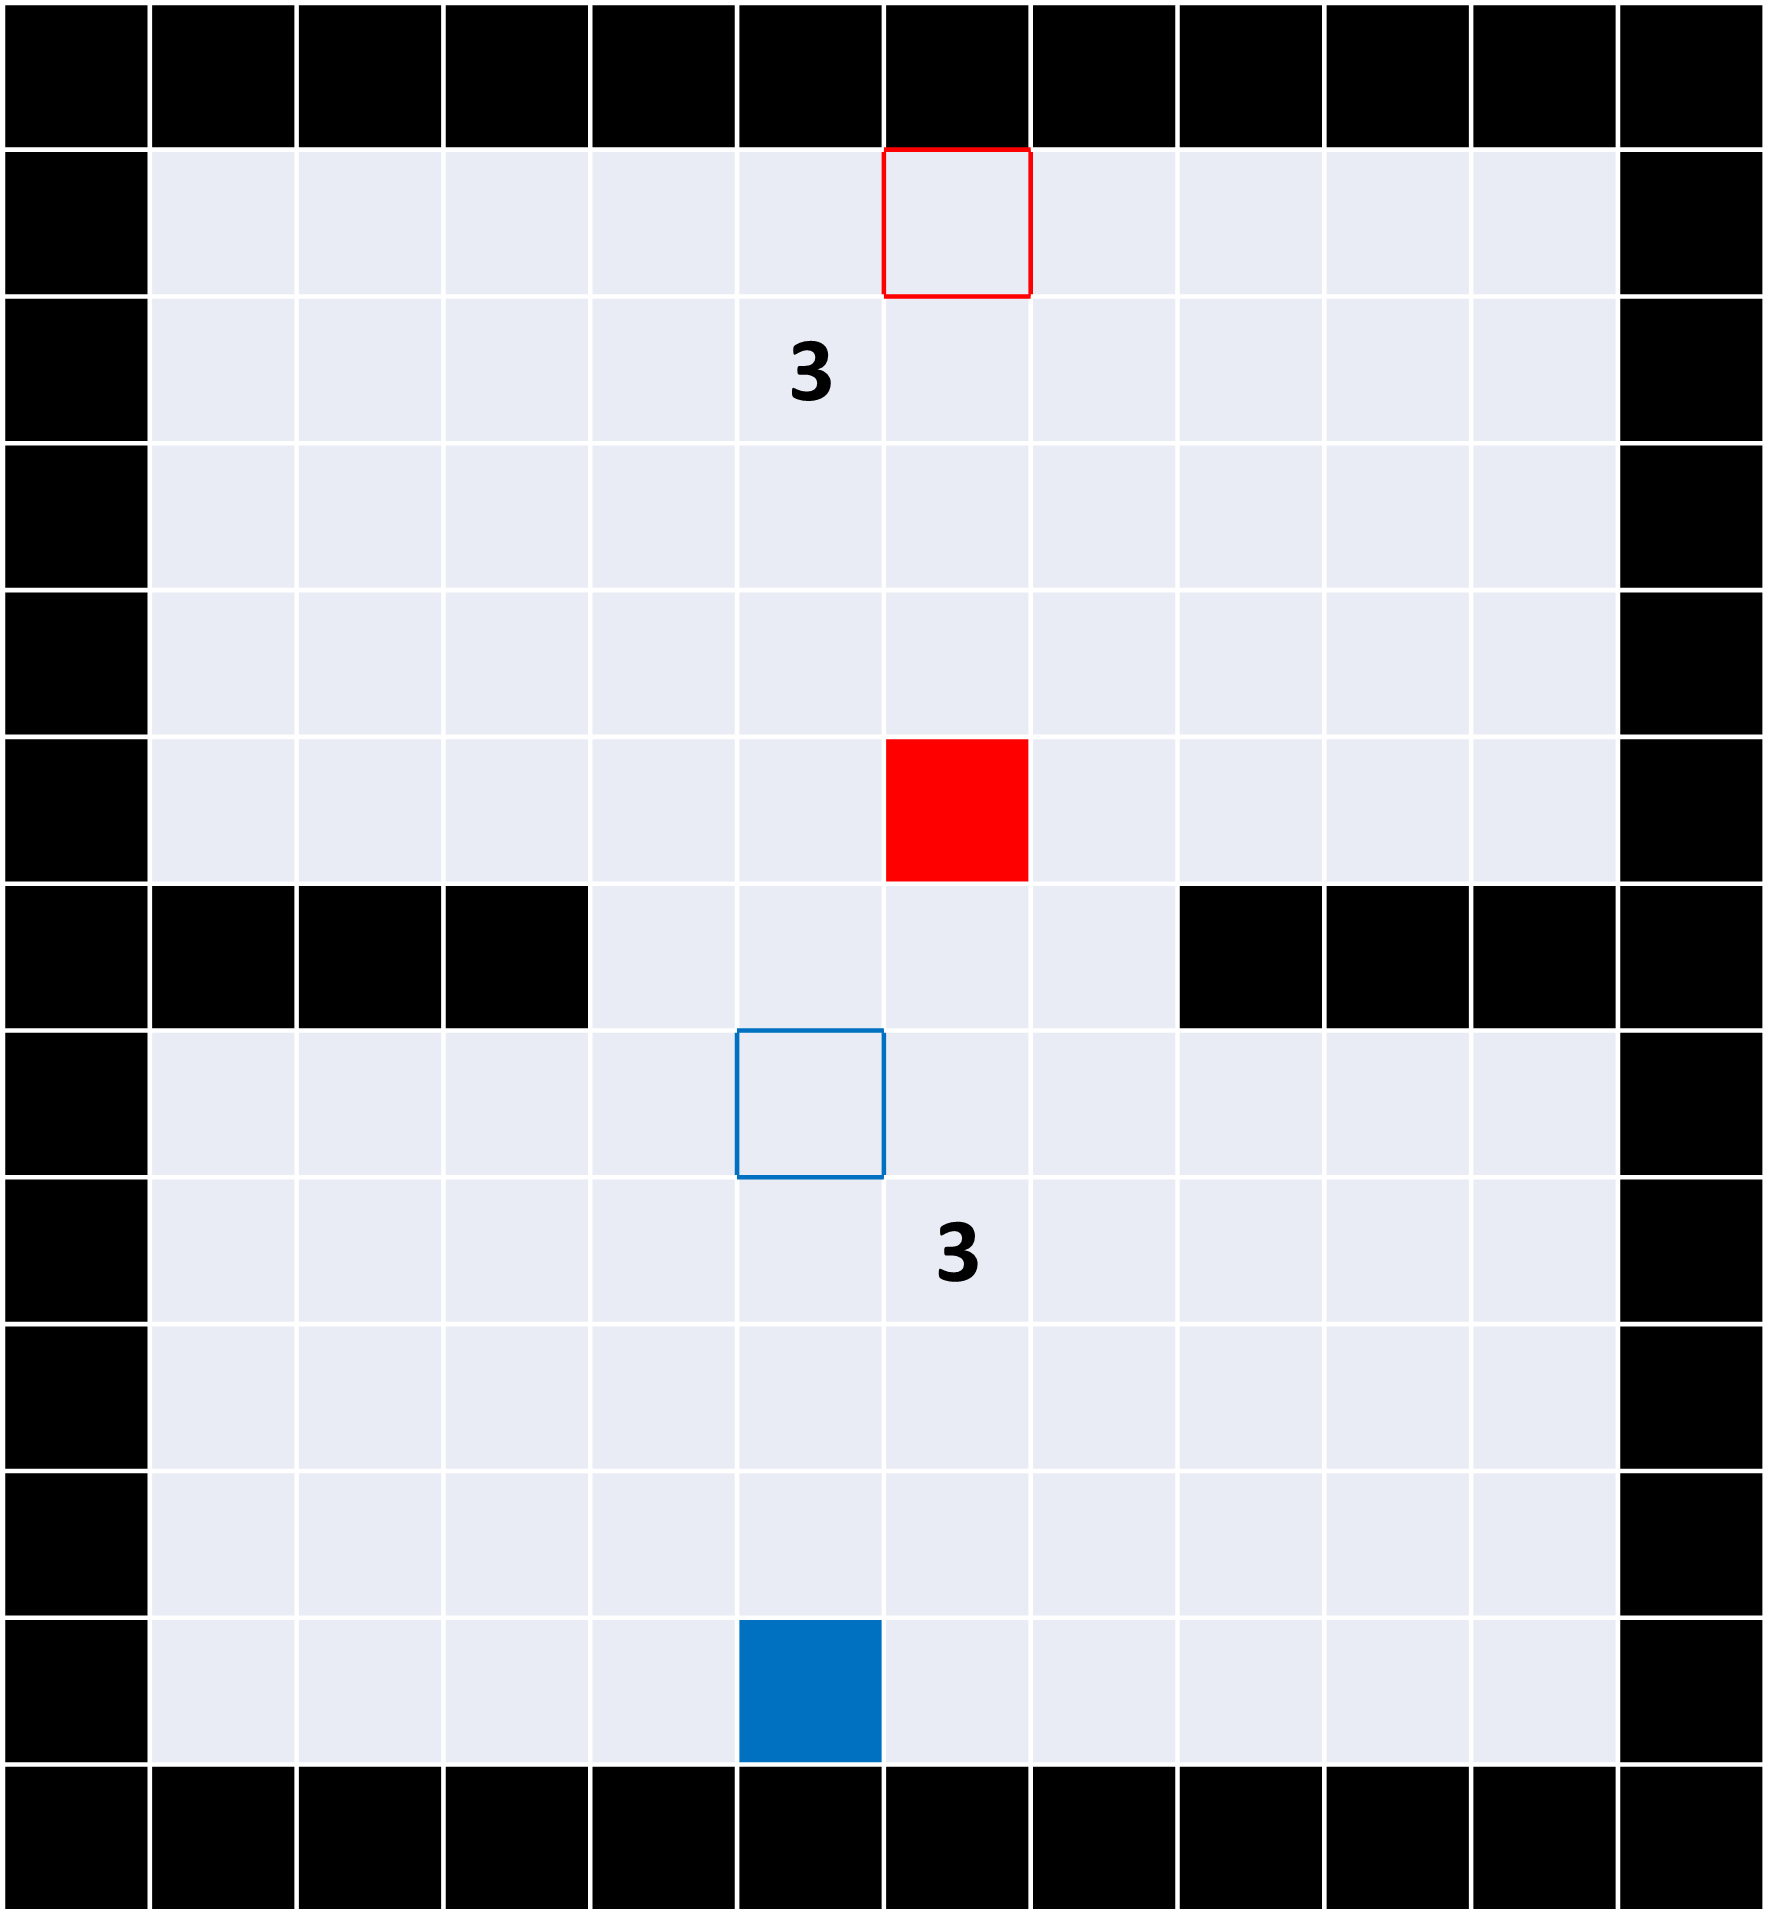
\includegraphics[width=0.12\textwidth]{Images/P1.png}
%         \label{subfig:m1}} 
%     \subfigure[$M_2$]{
%         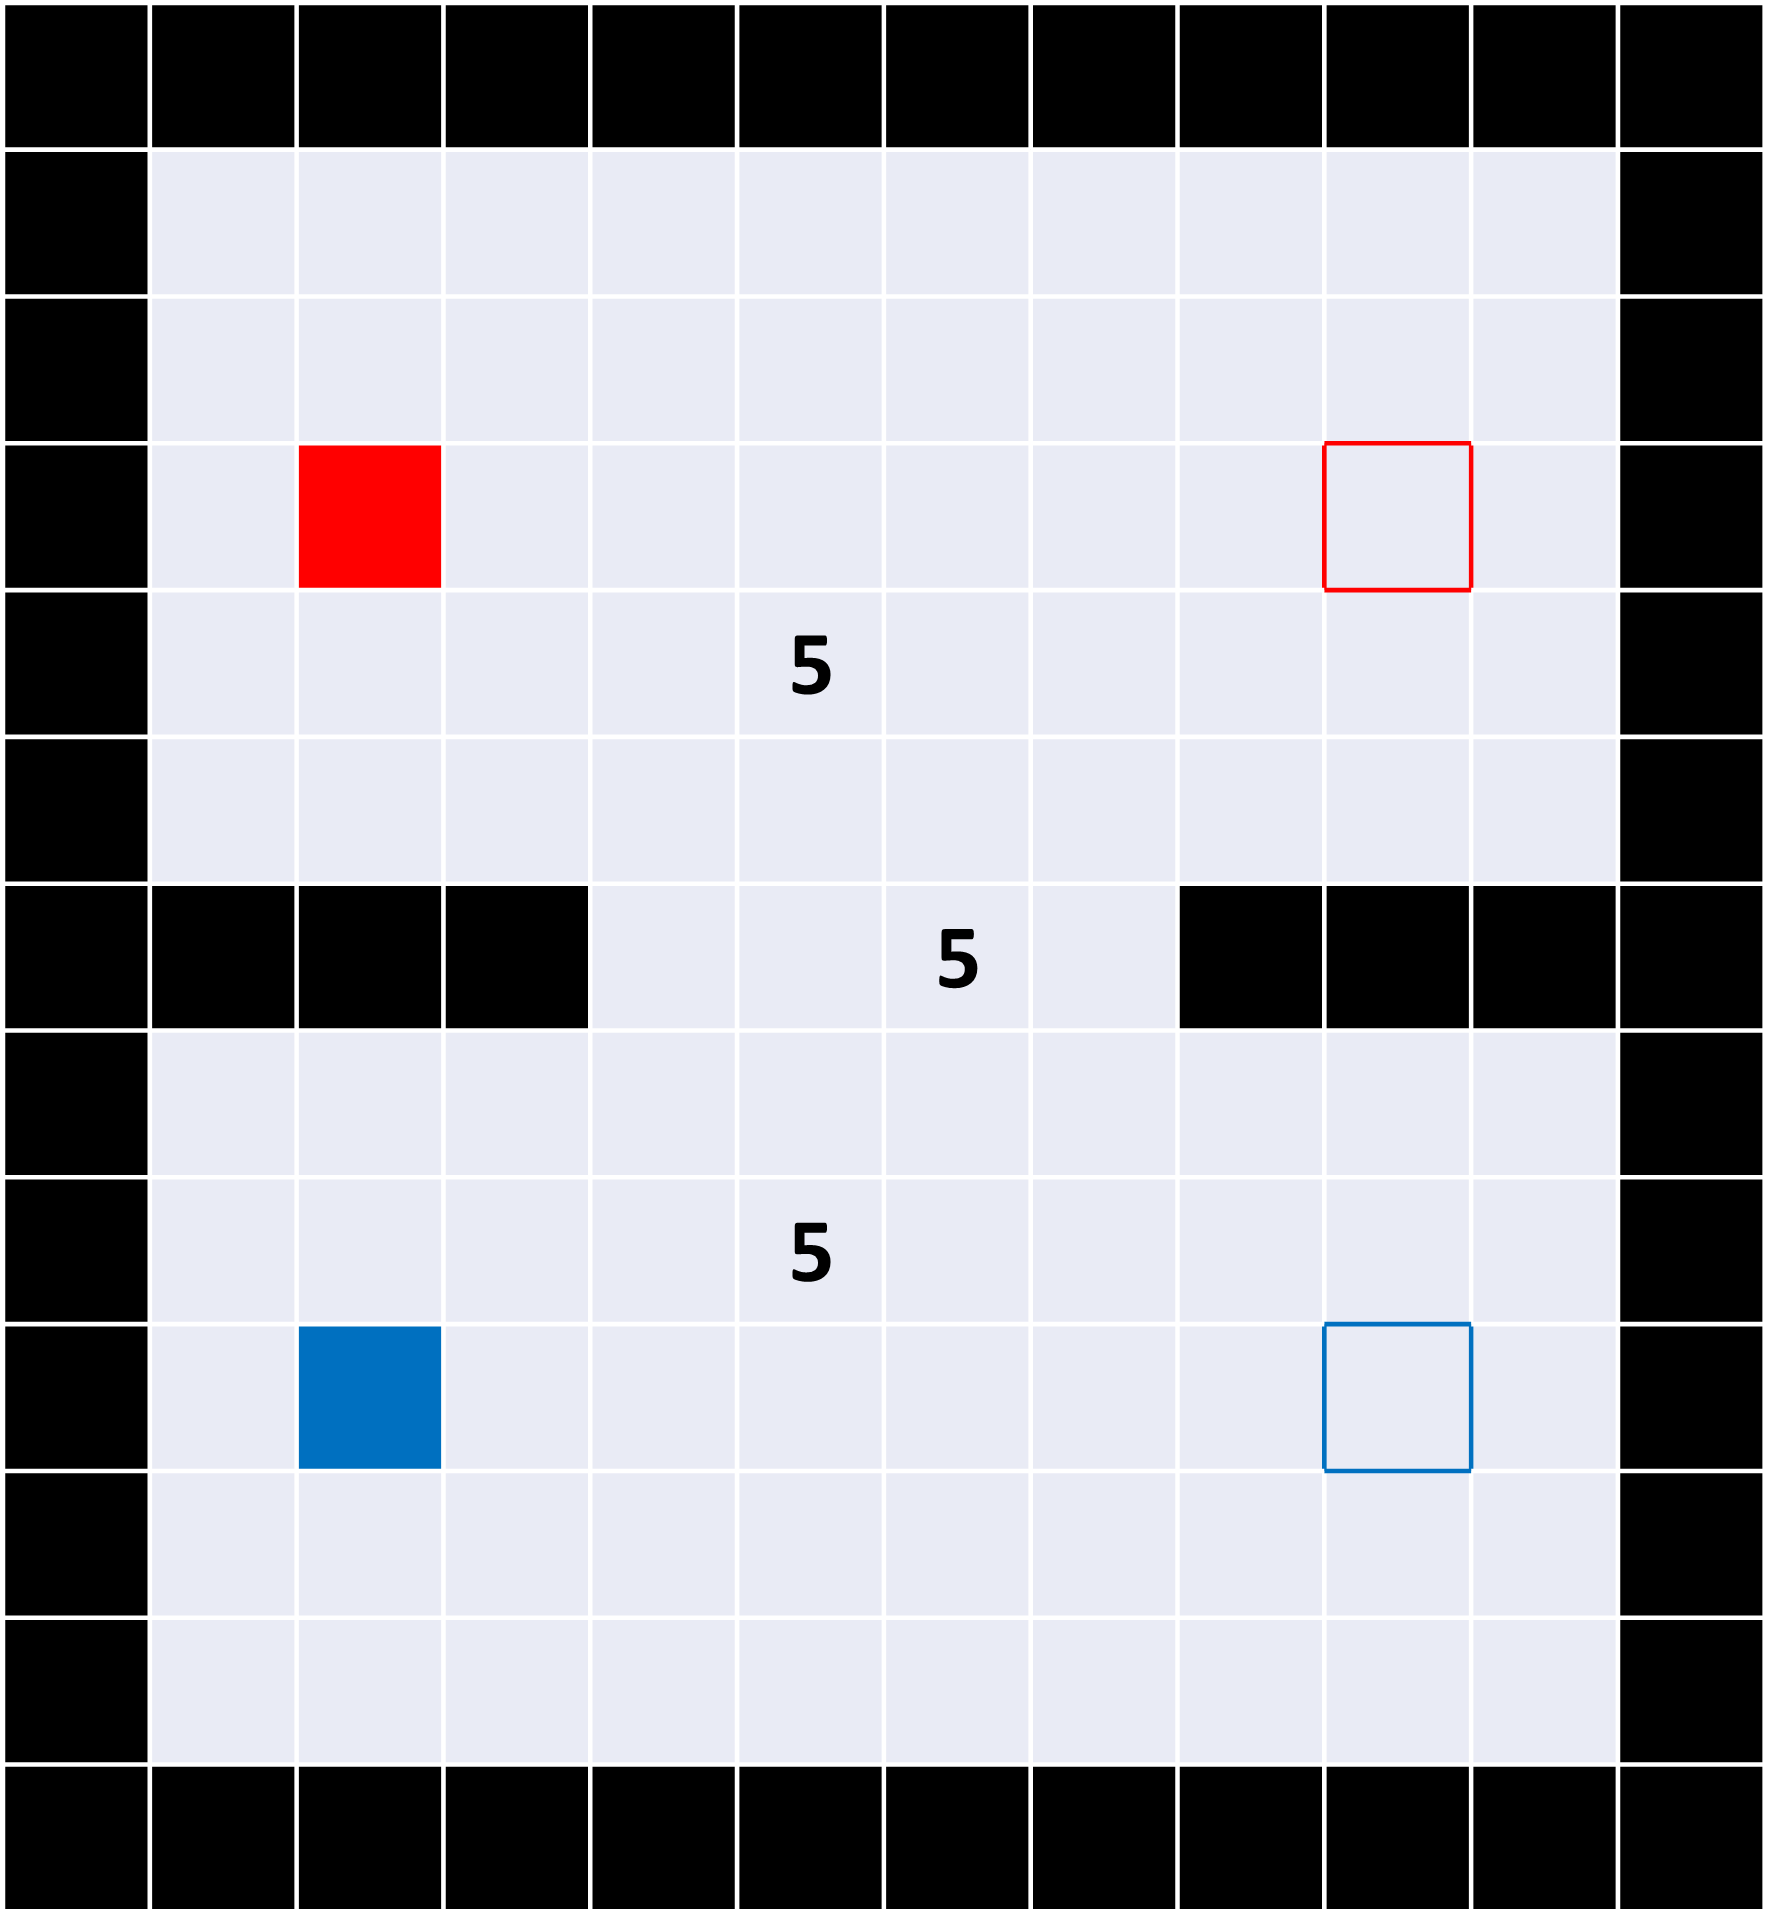
\includegraphics[width=0.12\textwidth]{Images/P2.png}
%         \label{subfig:m2}} 
%     \subfigure[$M_3$]{
%         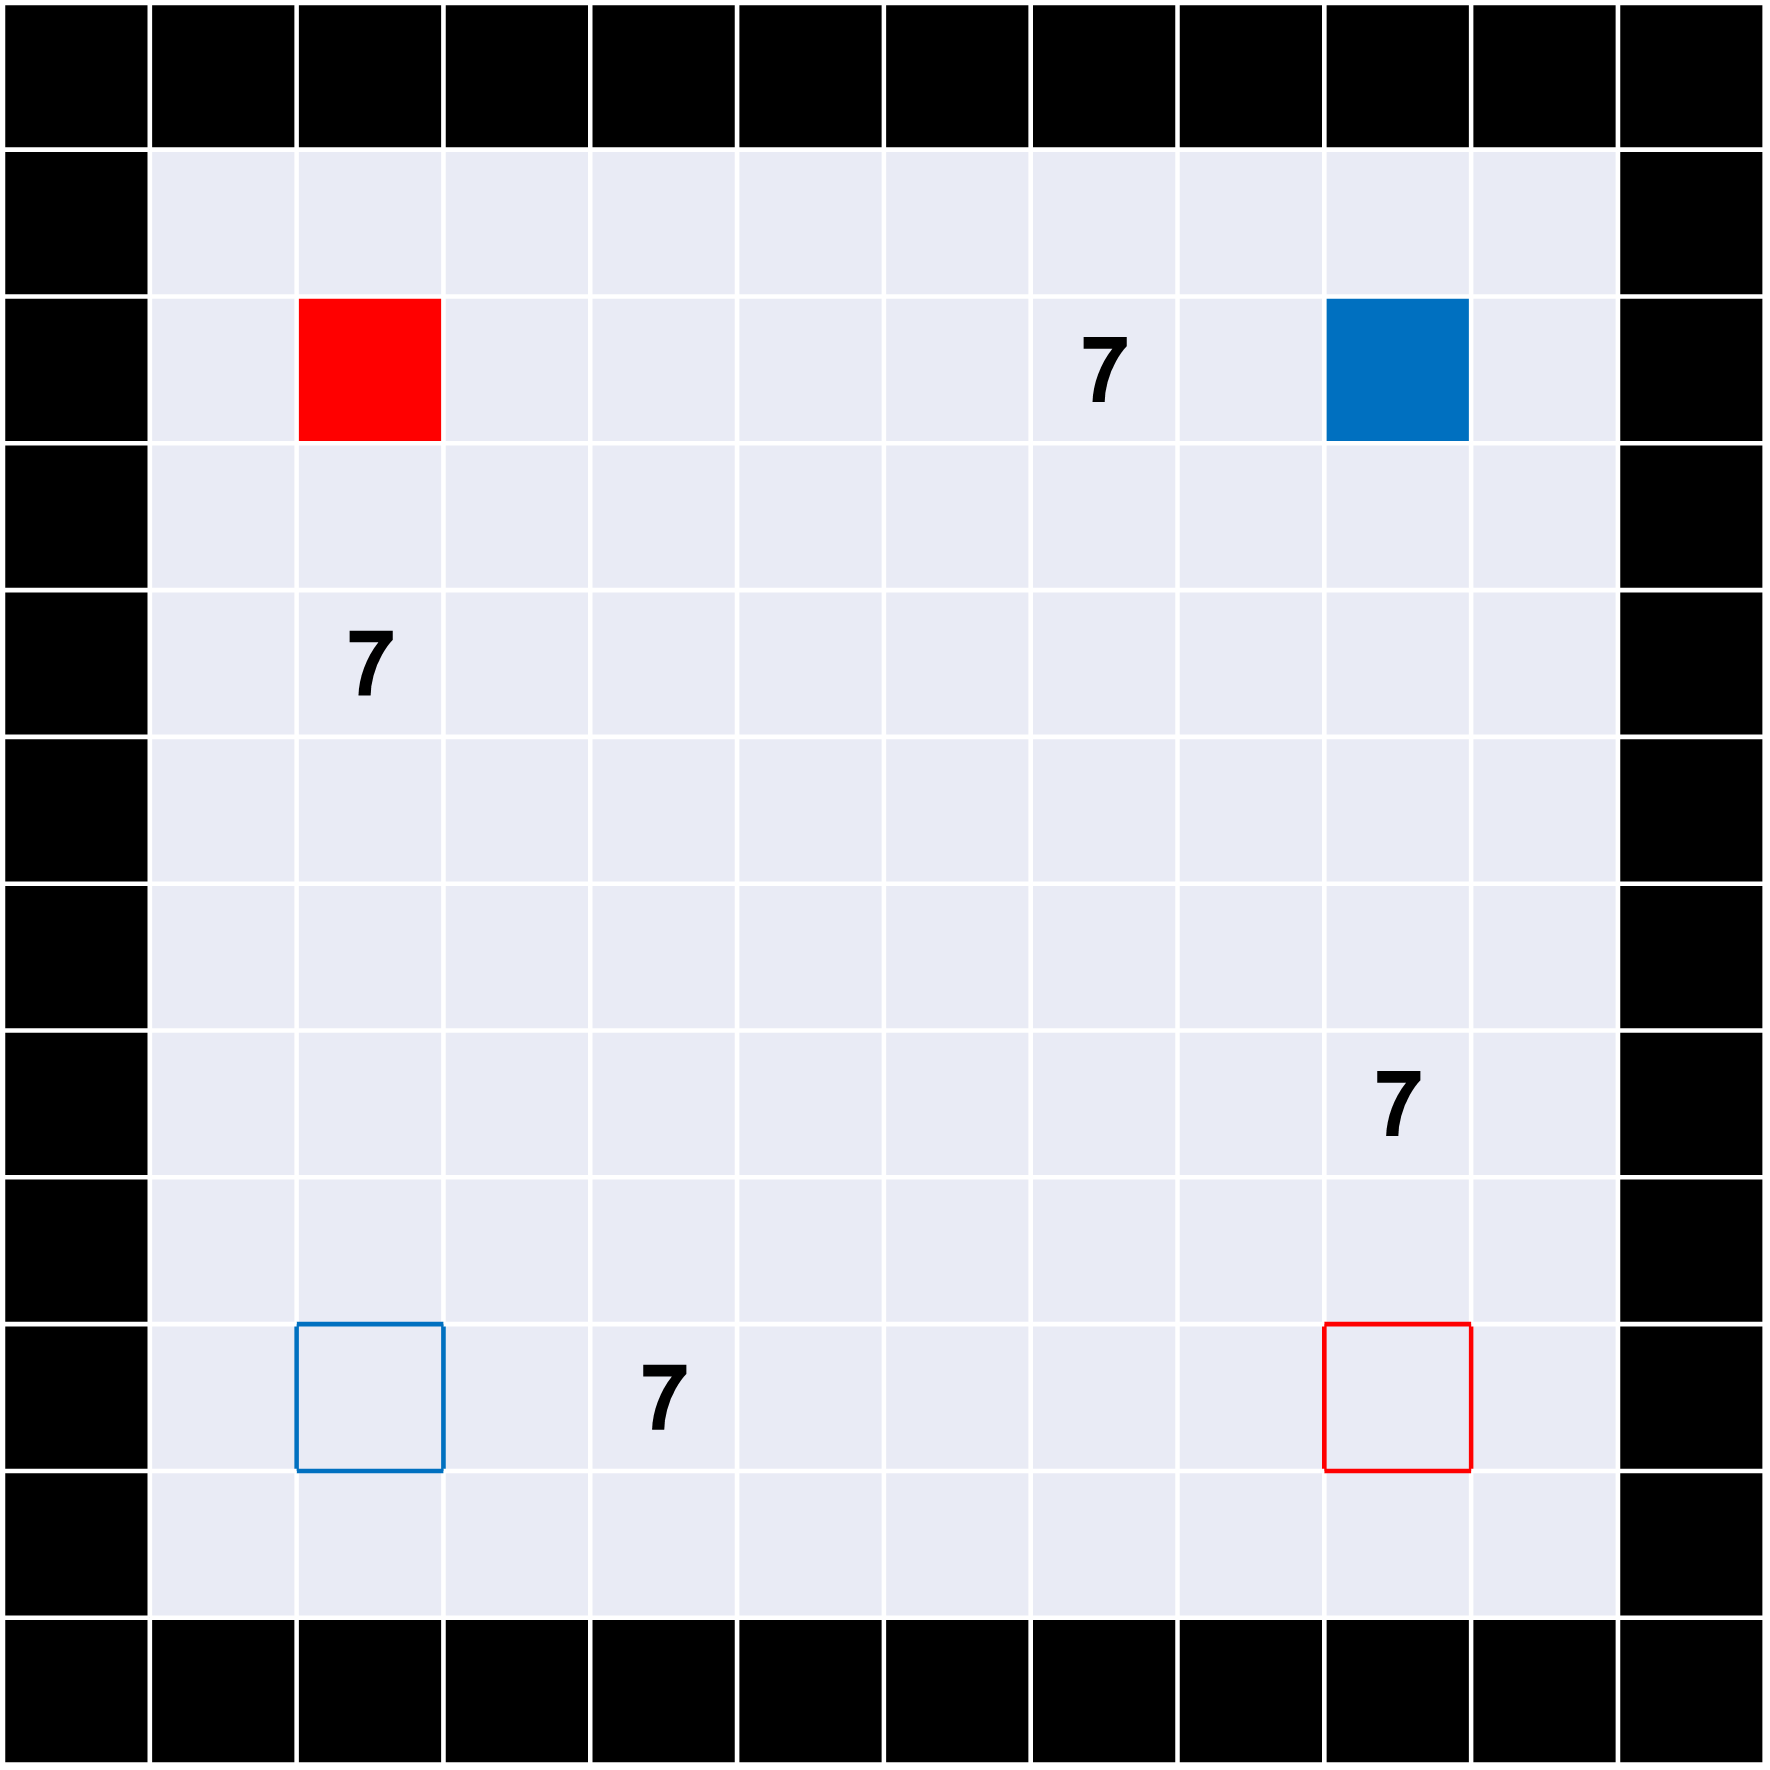
\includegraphics[width=0.13\textwidth]{Images/P3.png}
%         \label{subfig:m3}}
%     \subfigure[$M_4$]{
%         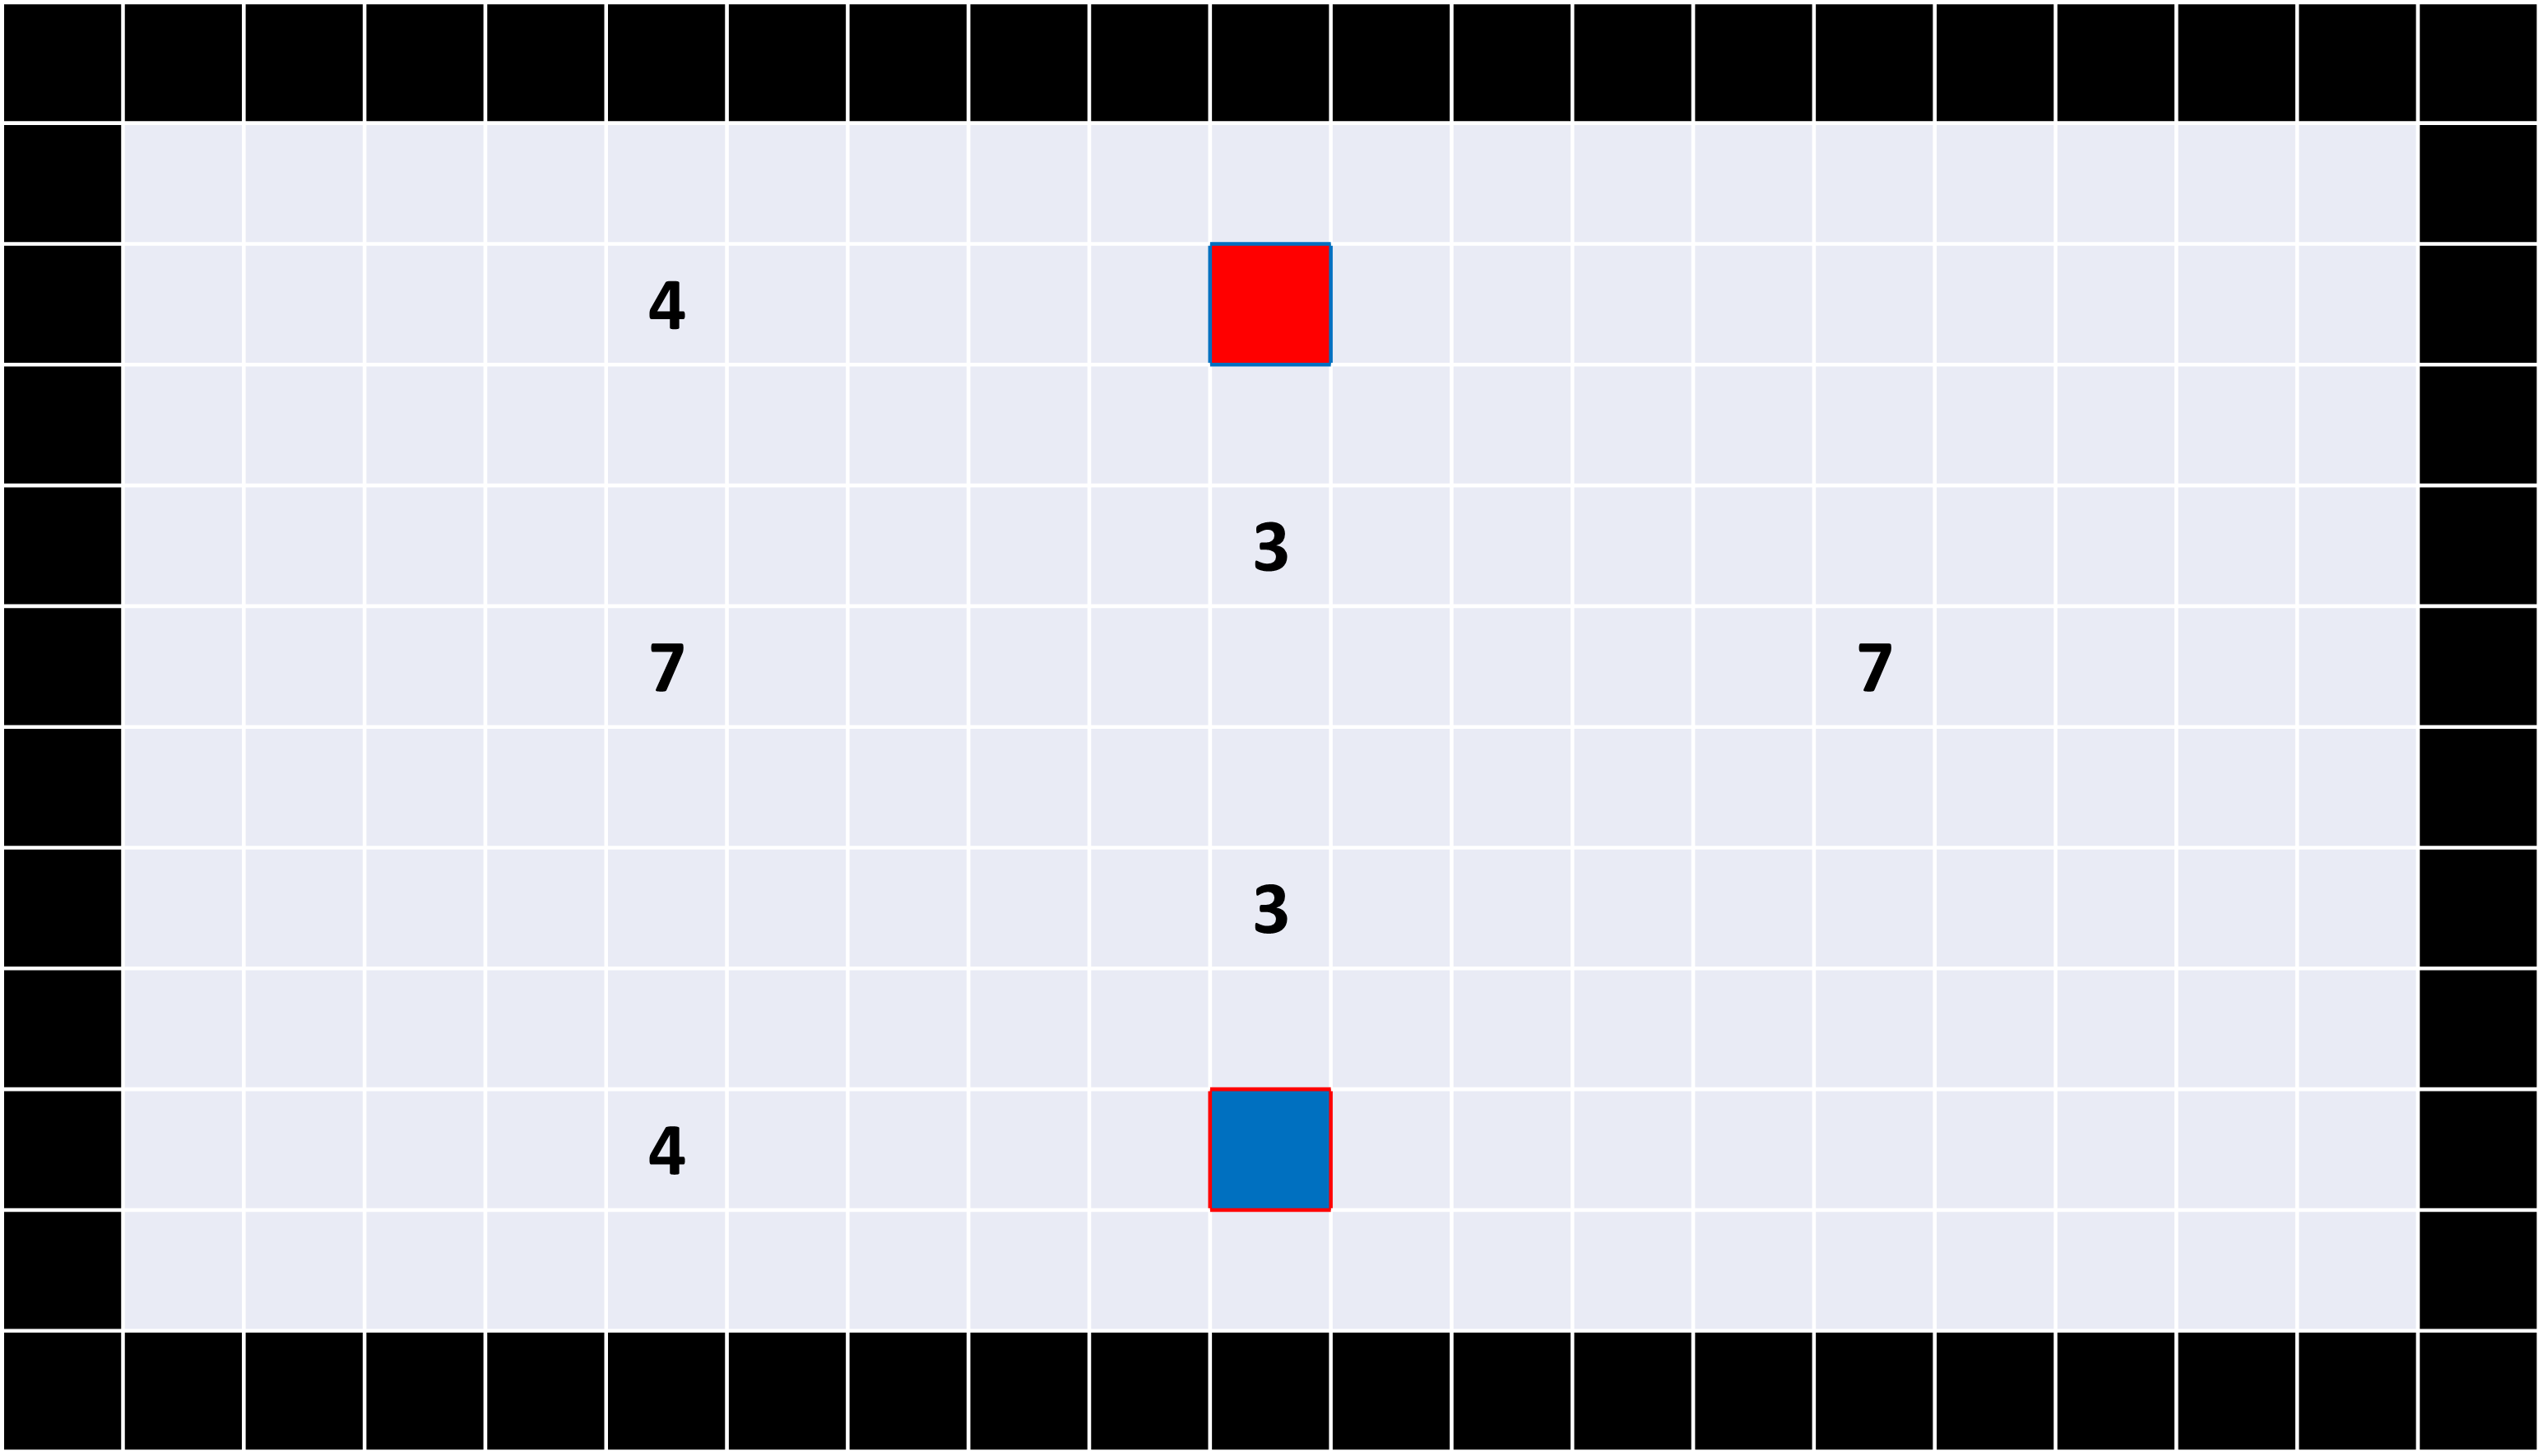
\includegraphics[width=0.245\textwidth]{Images/P4.png}
%         \label{subfig:m4}}
%     \subfigure[$M_5$]{
%         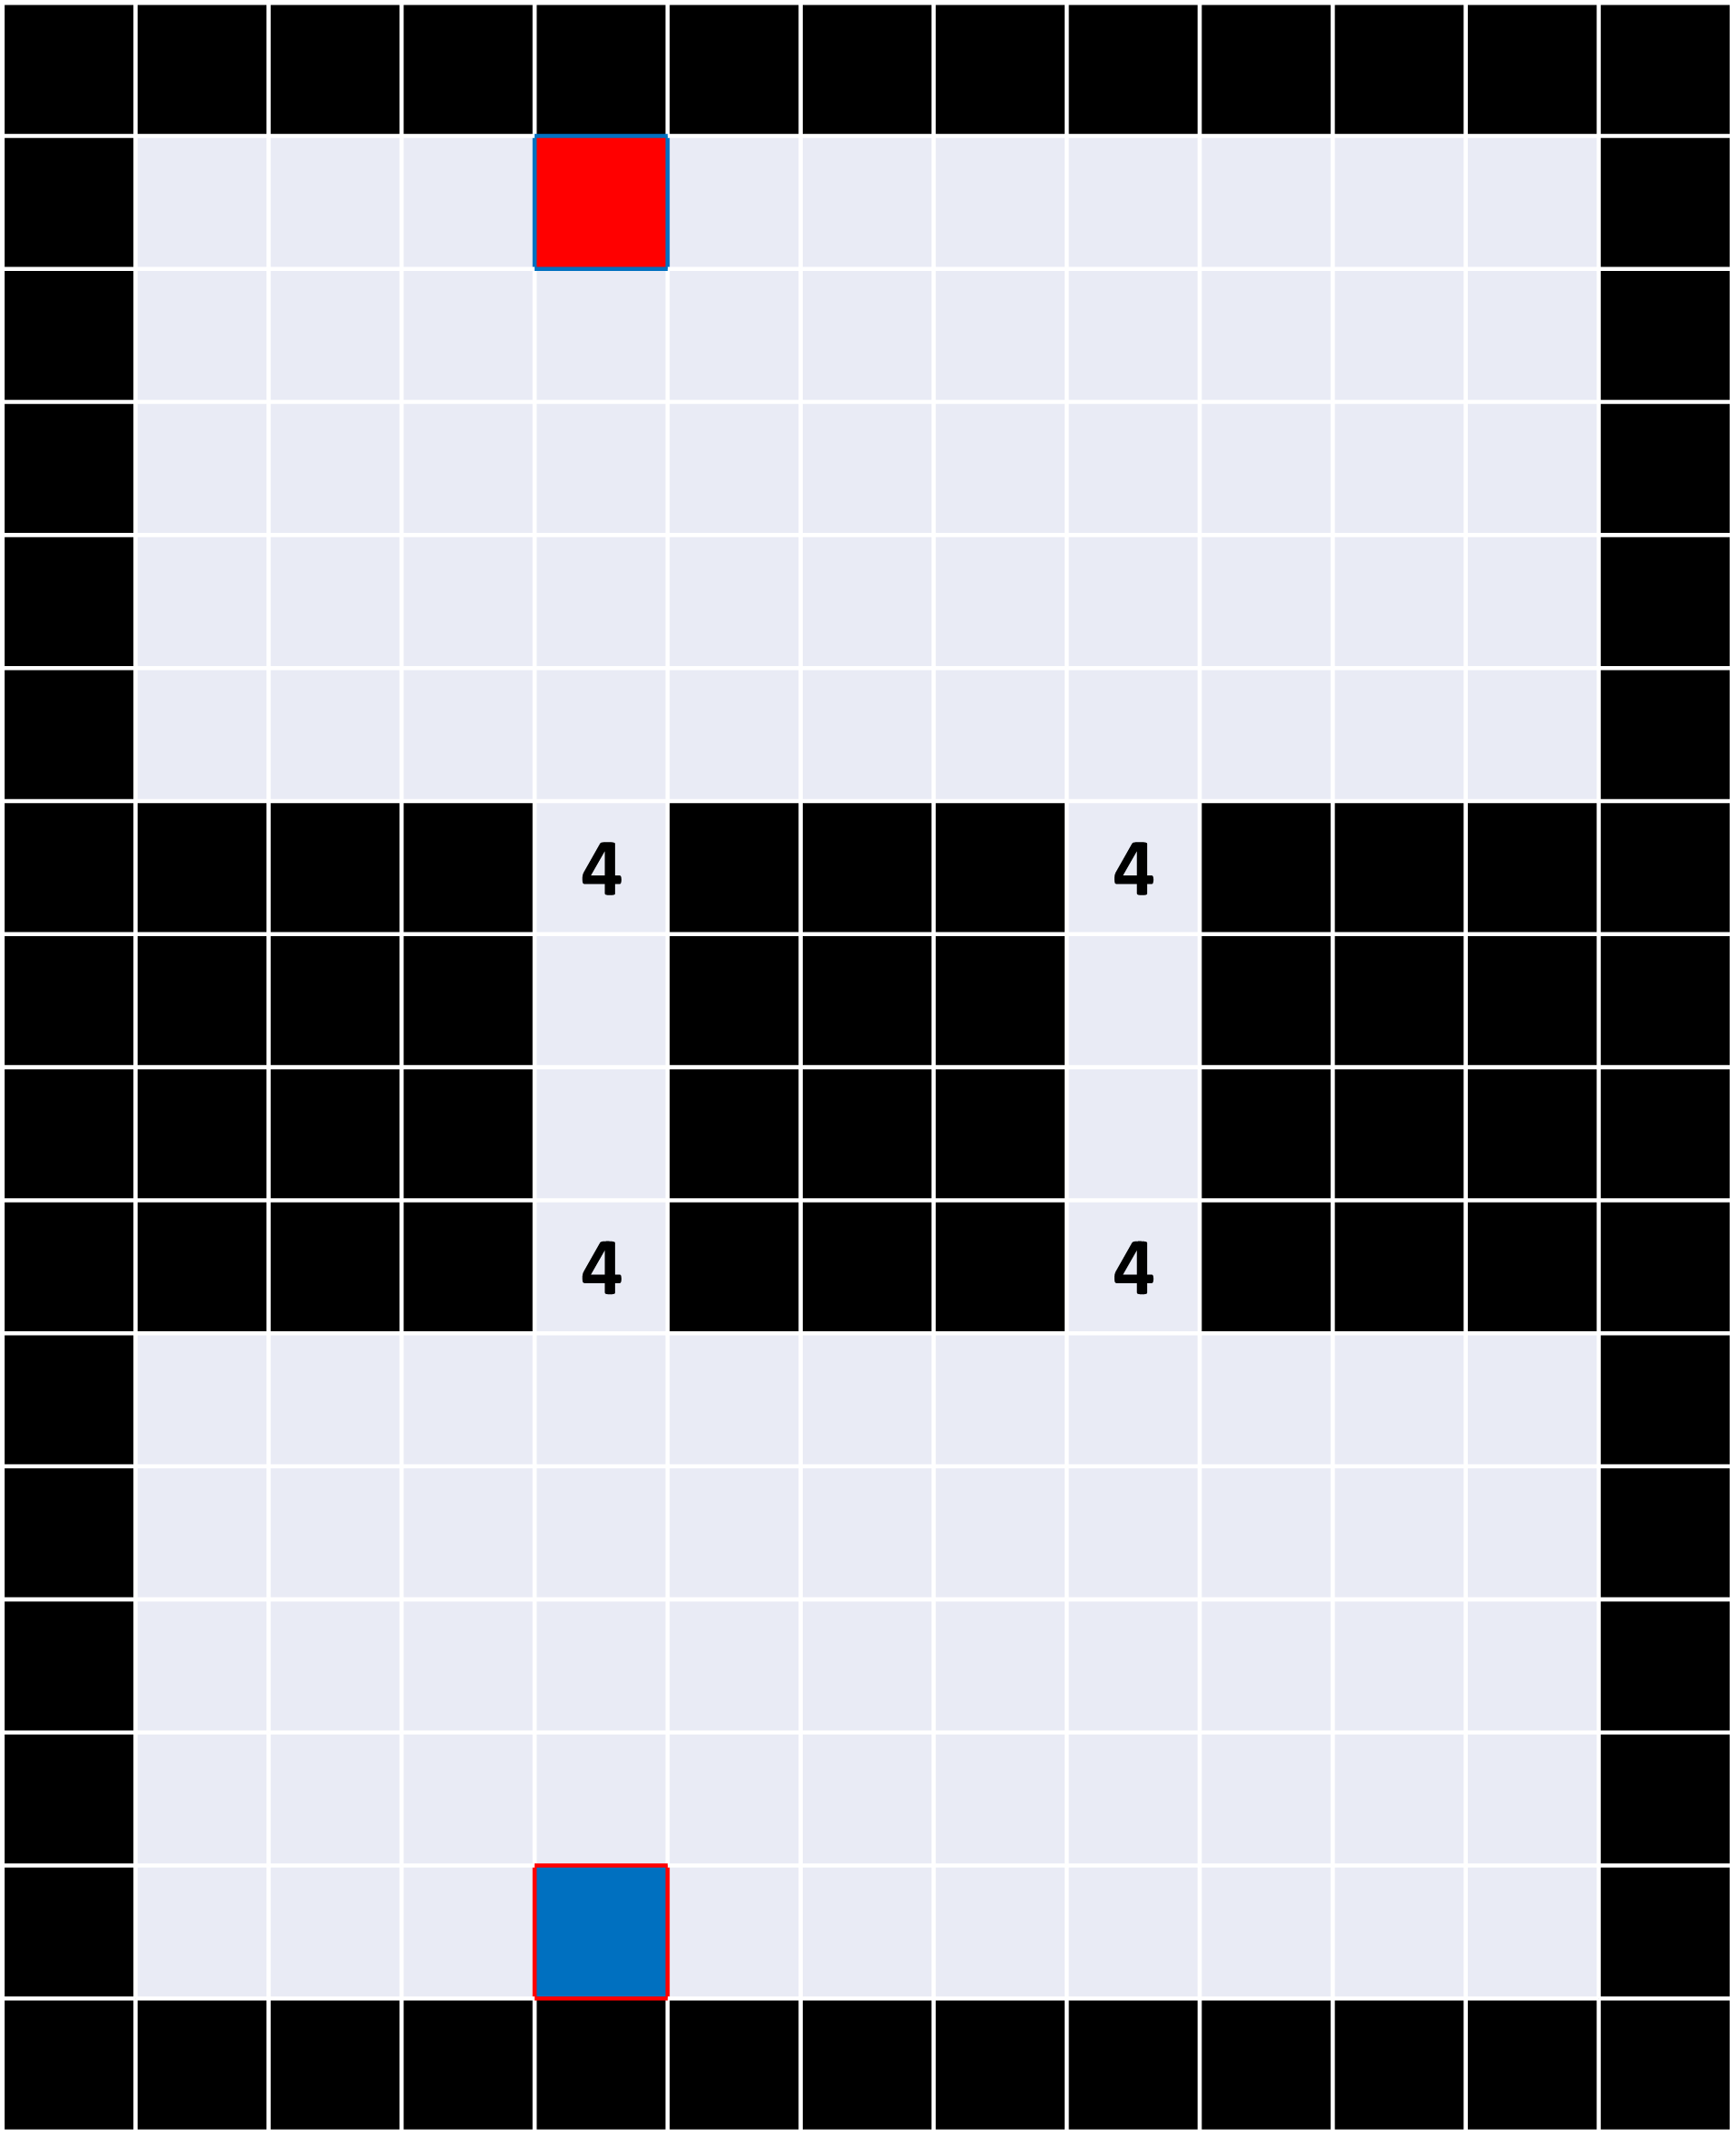
\includegraphics[width=0.115\textwidth]{Images/P5.png}
%         \label{subfig:m5}}
%     % \caption{2 agents' benchmarks used in the empirical evaluation. Each color represents an agent, where the filled cells are the agents' initial states and the bordered cells are the agents' goal states. Black cells are blocked. The numbers within cells represent beacons with respective influence range, located in those cells.}
%     % \label{fig:big-problems}
%      \subfigure[$L_1$]{
%         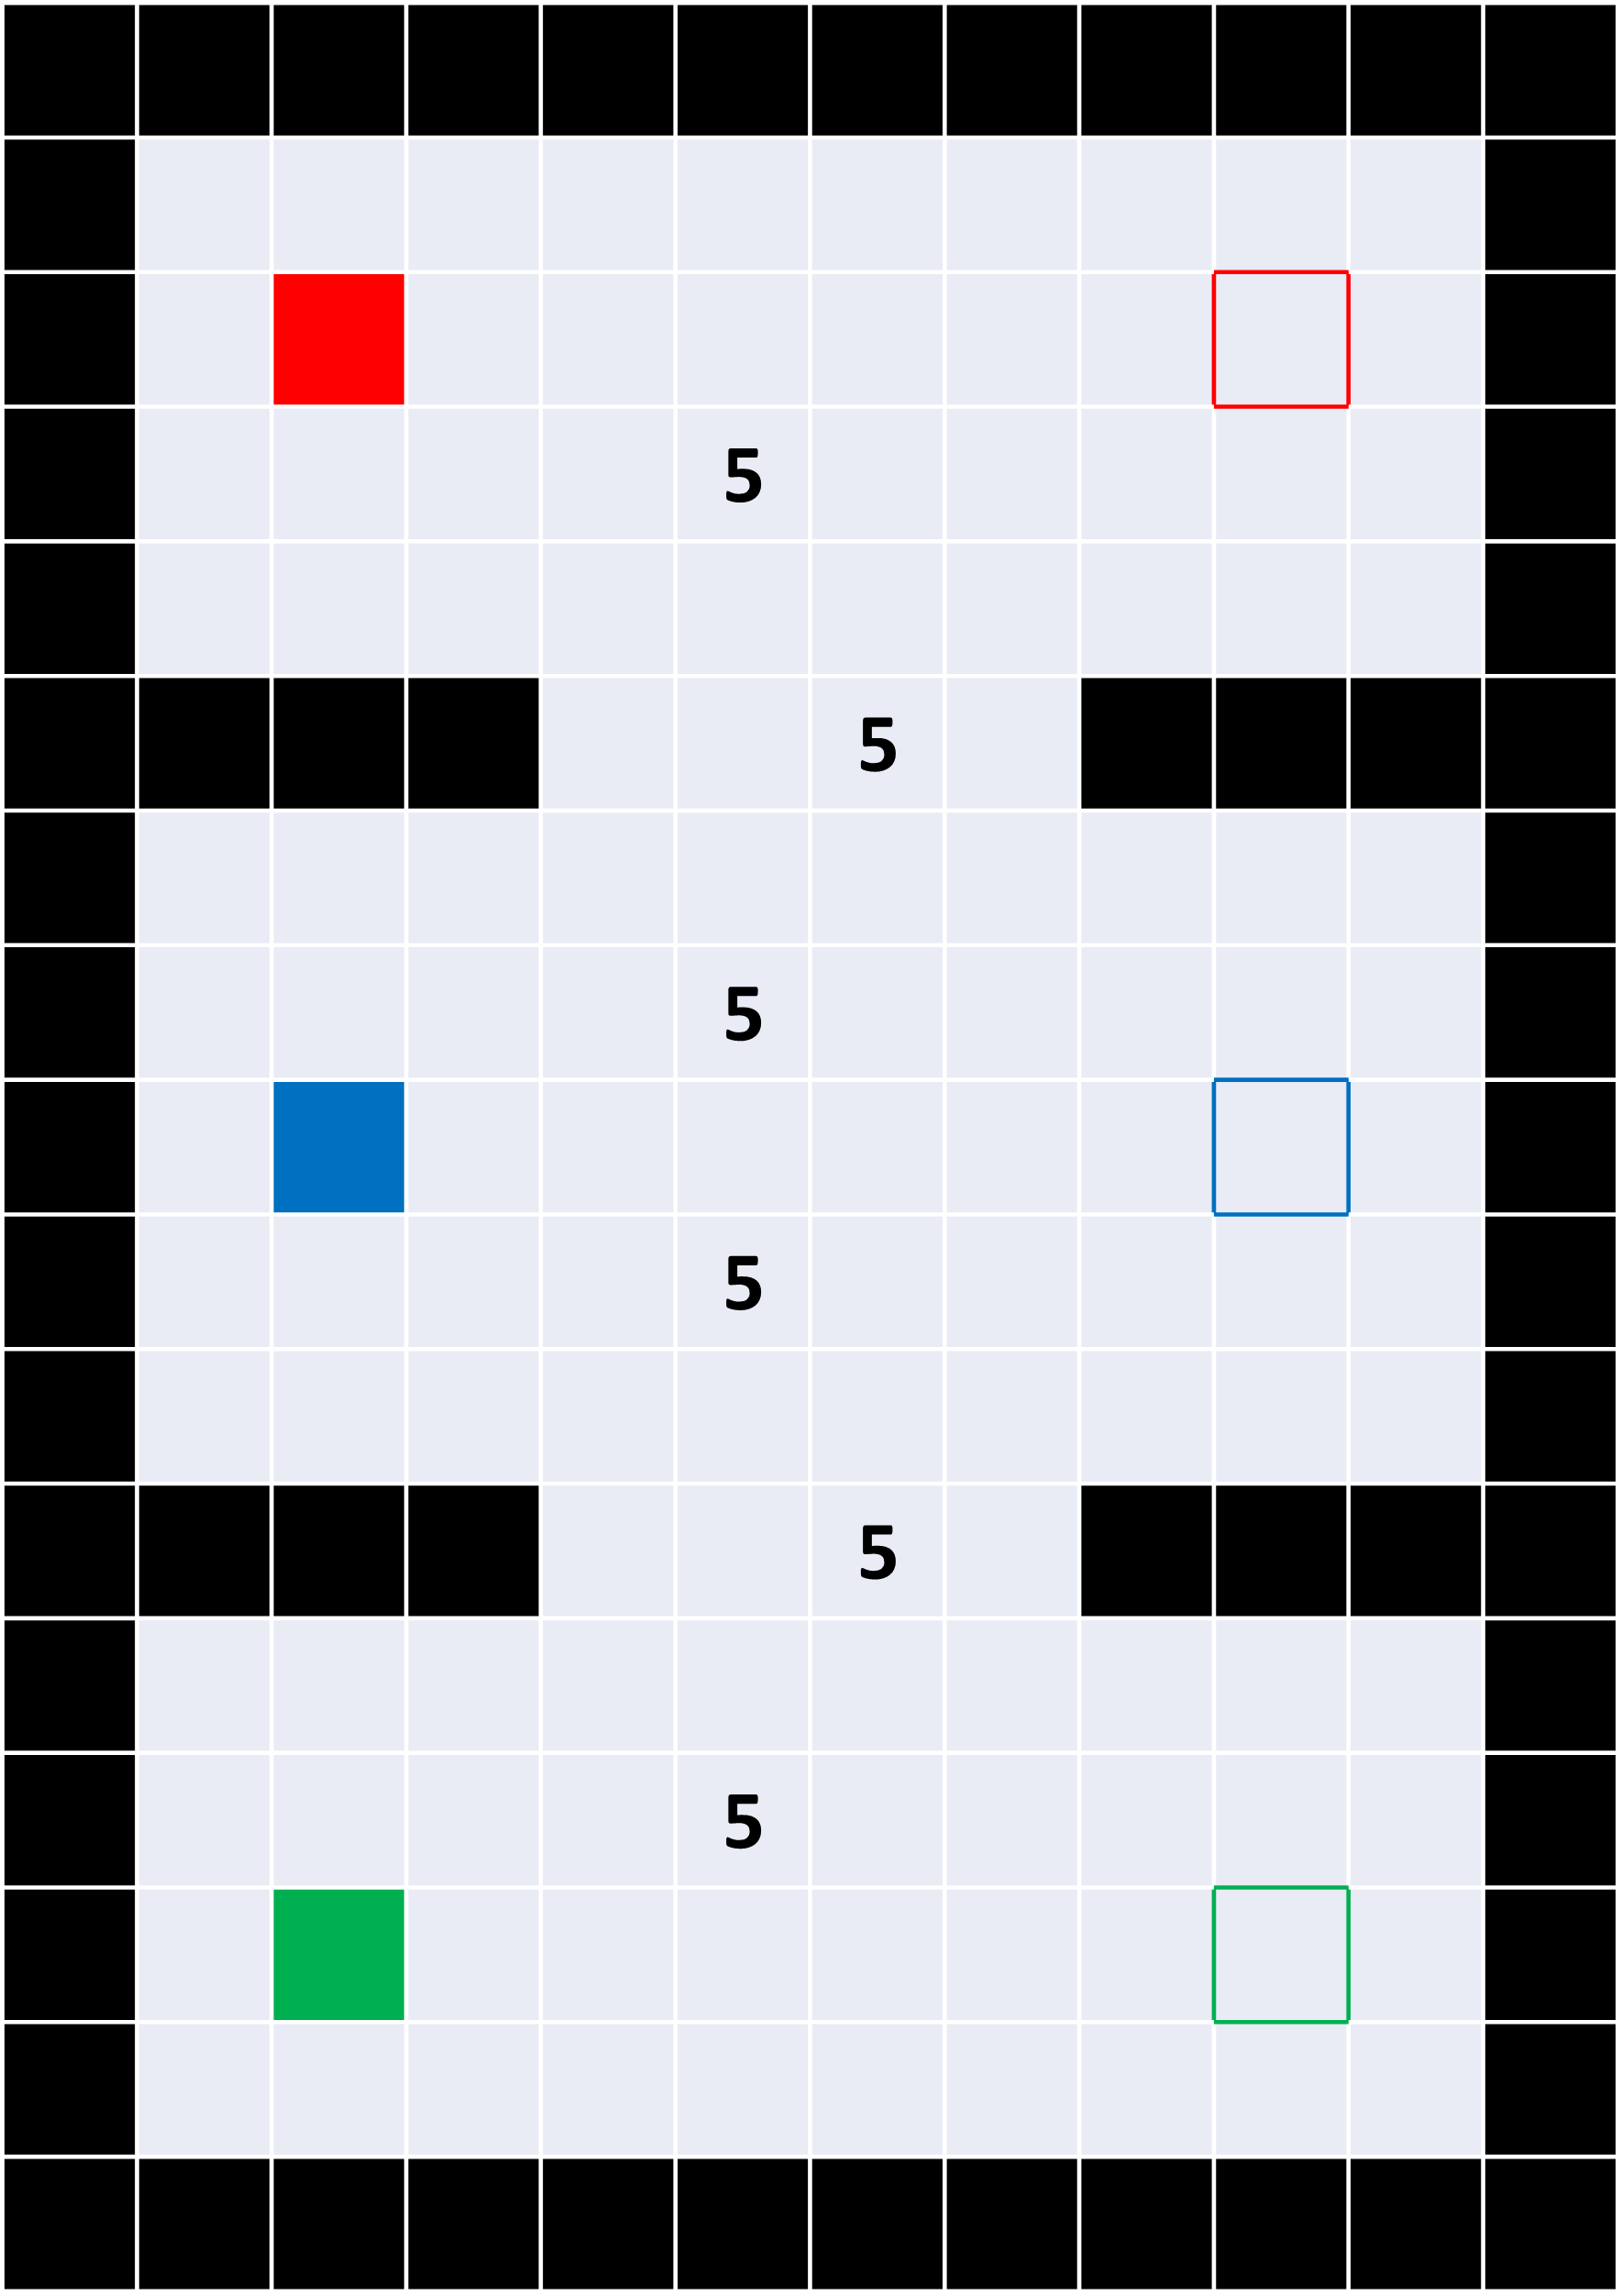
\includegraphics[width=0.1\textwidth]{Images/P2-3a.png}
%         \label{subfig:l1}}
%     \subfigure[$L_2$]{
%         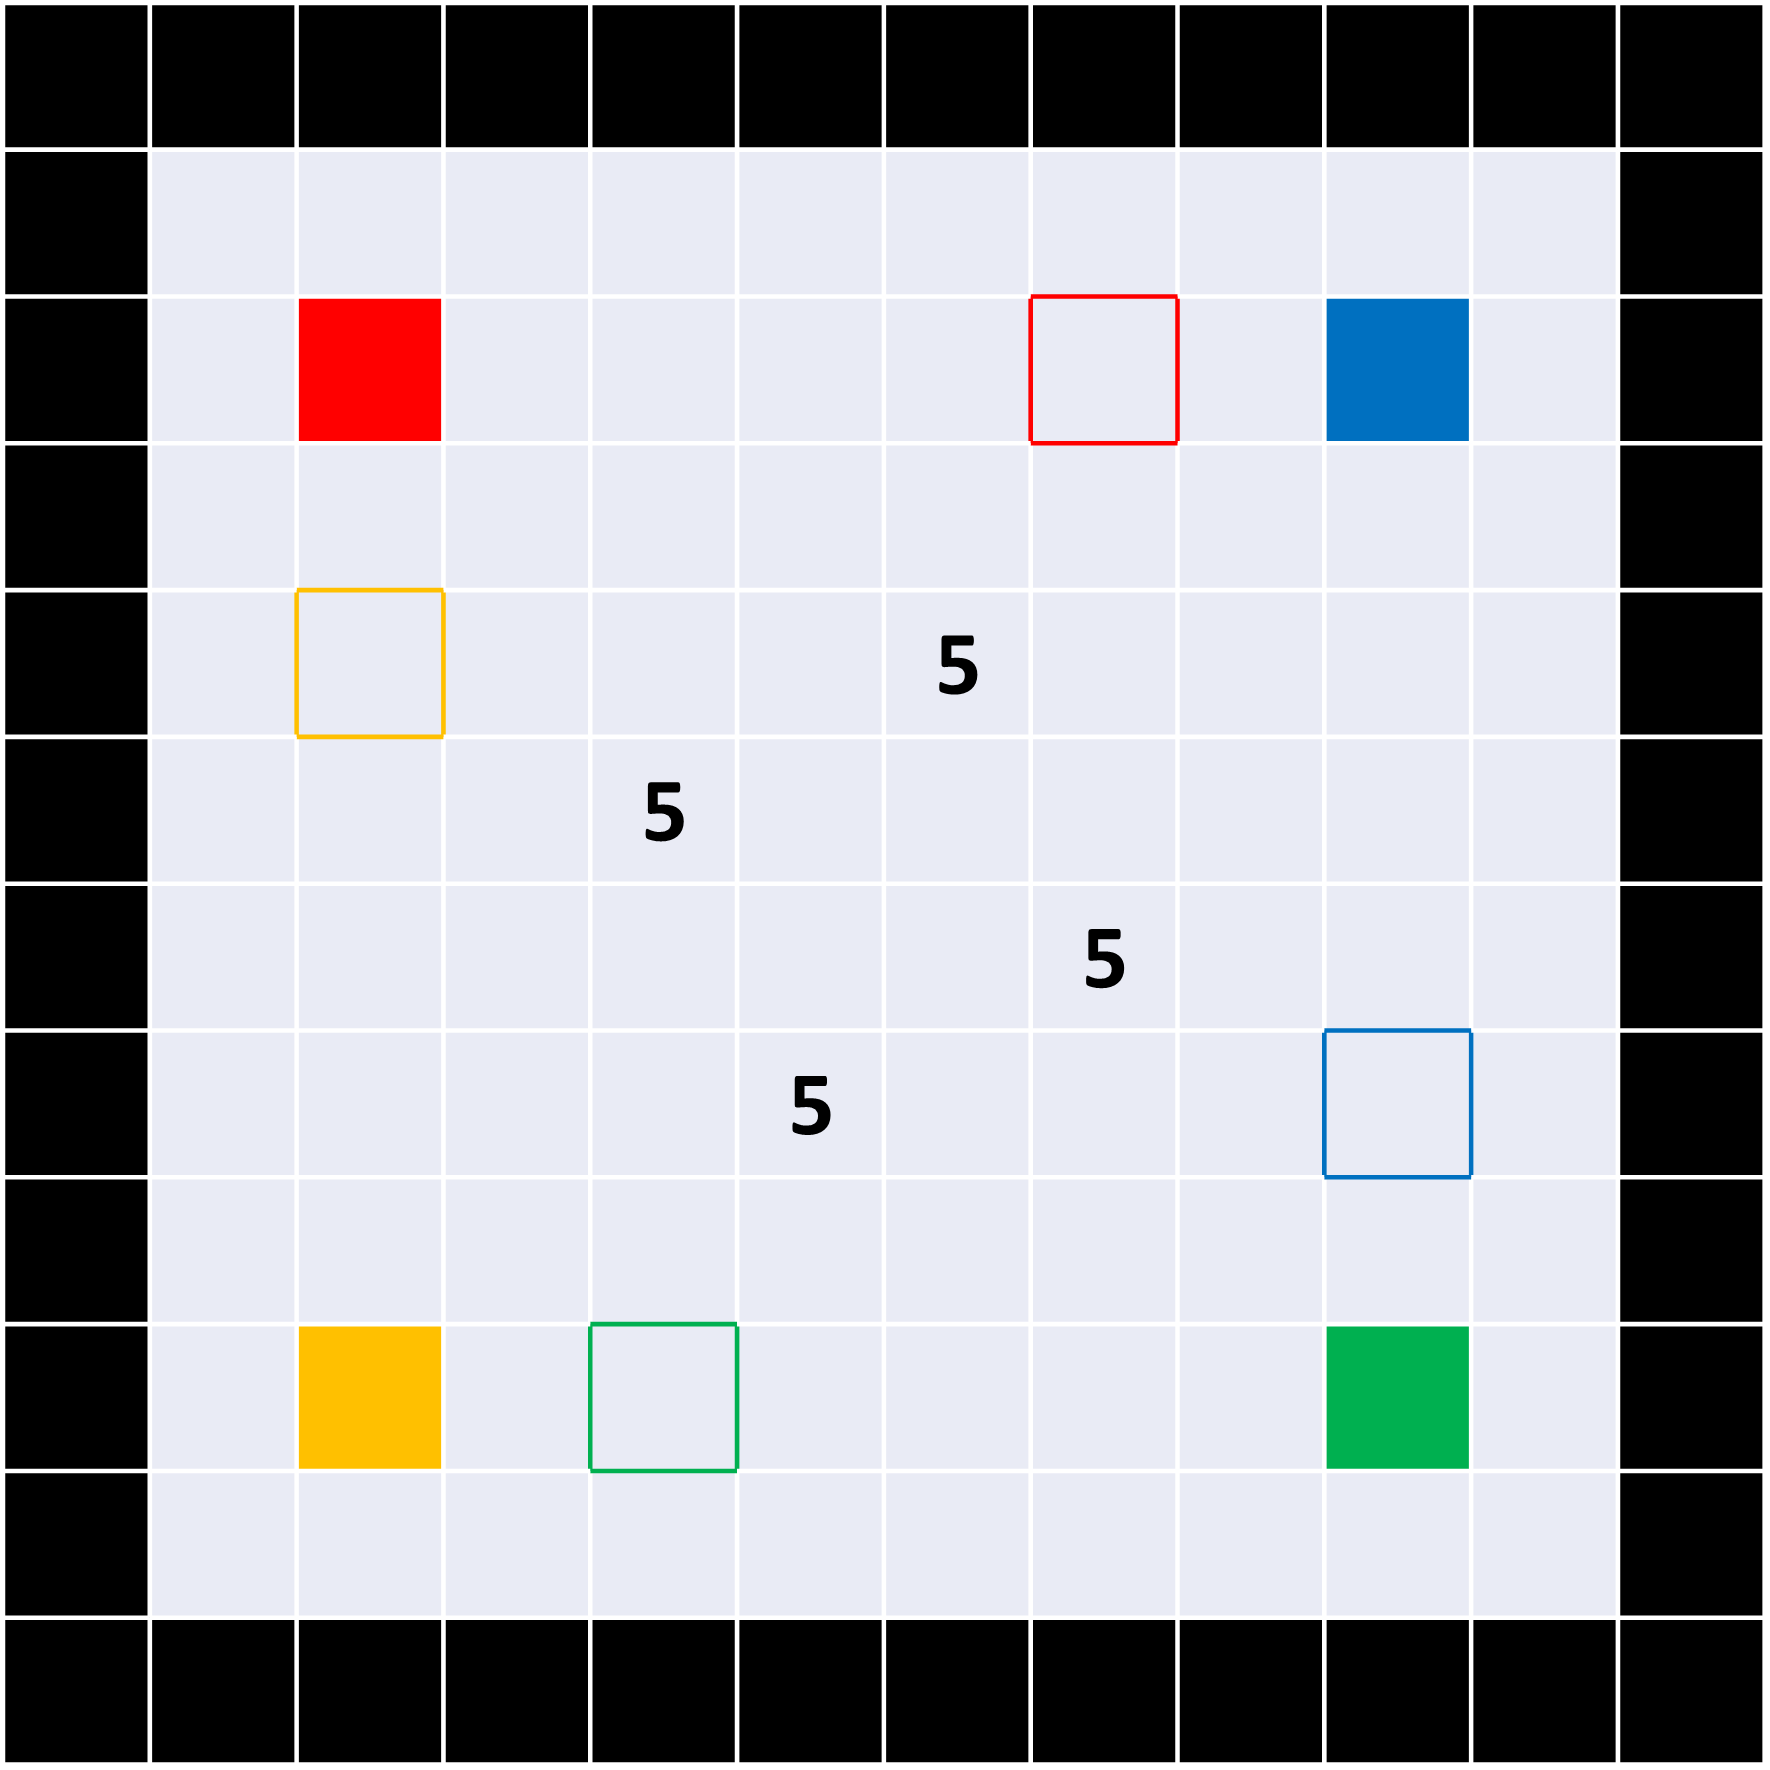
\includegraphics[width=0.1425\textwidth]{Images/P3-4a.png}
%         \label{subfig:l2}}
%     \subfigure[$L_3$]{
%         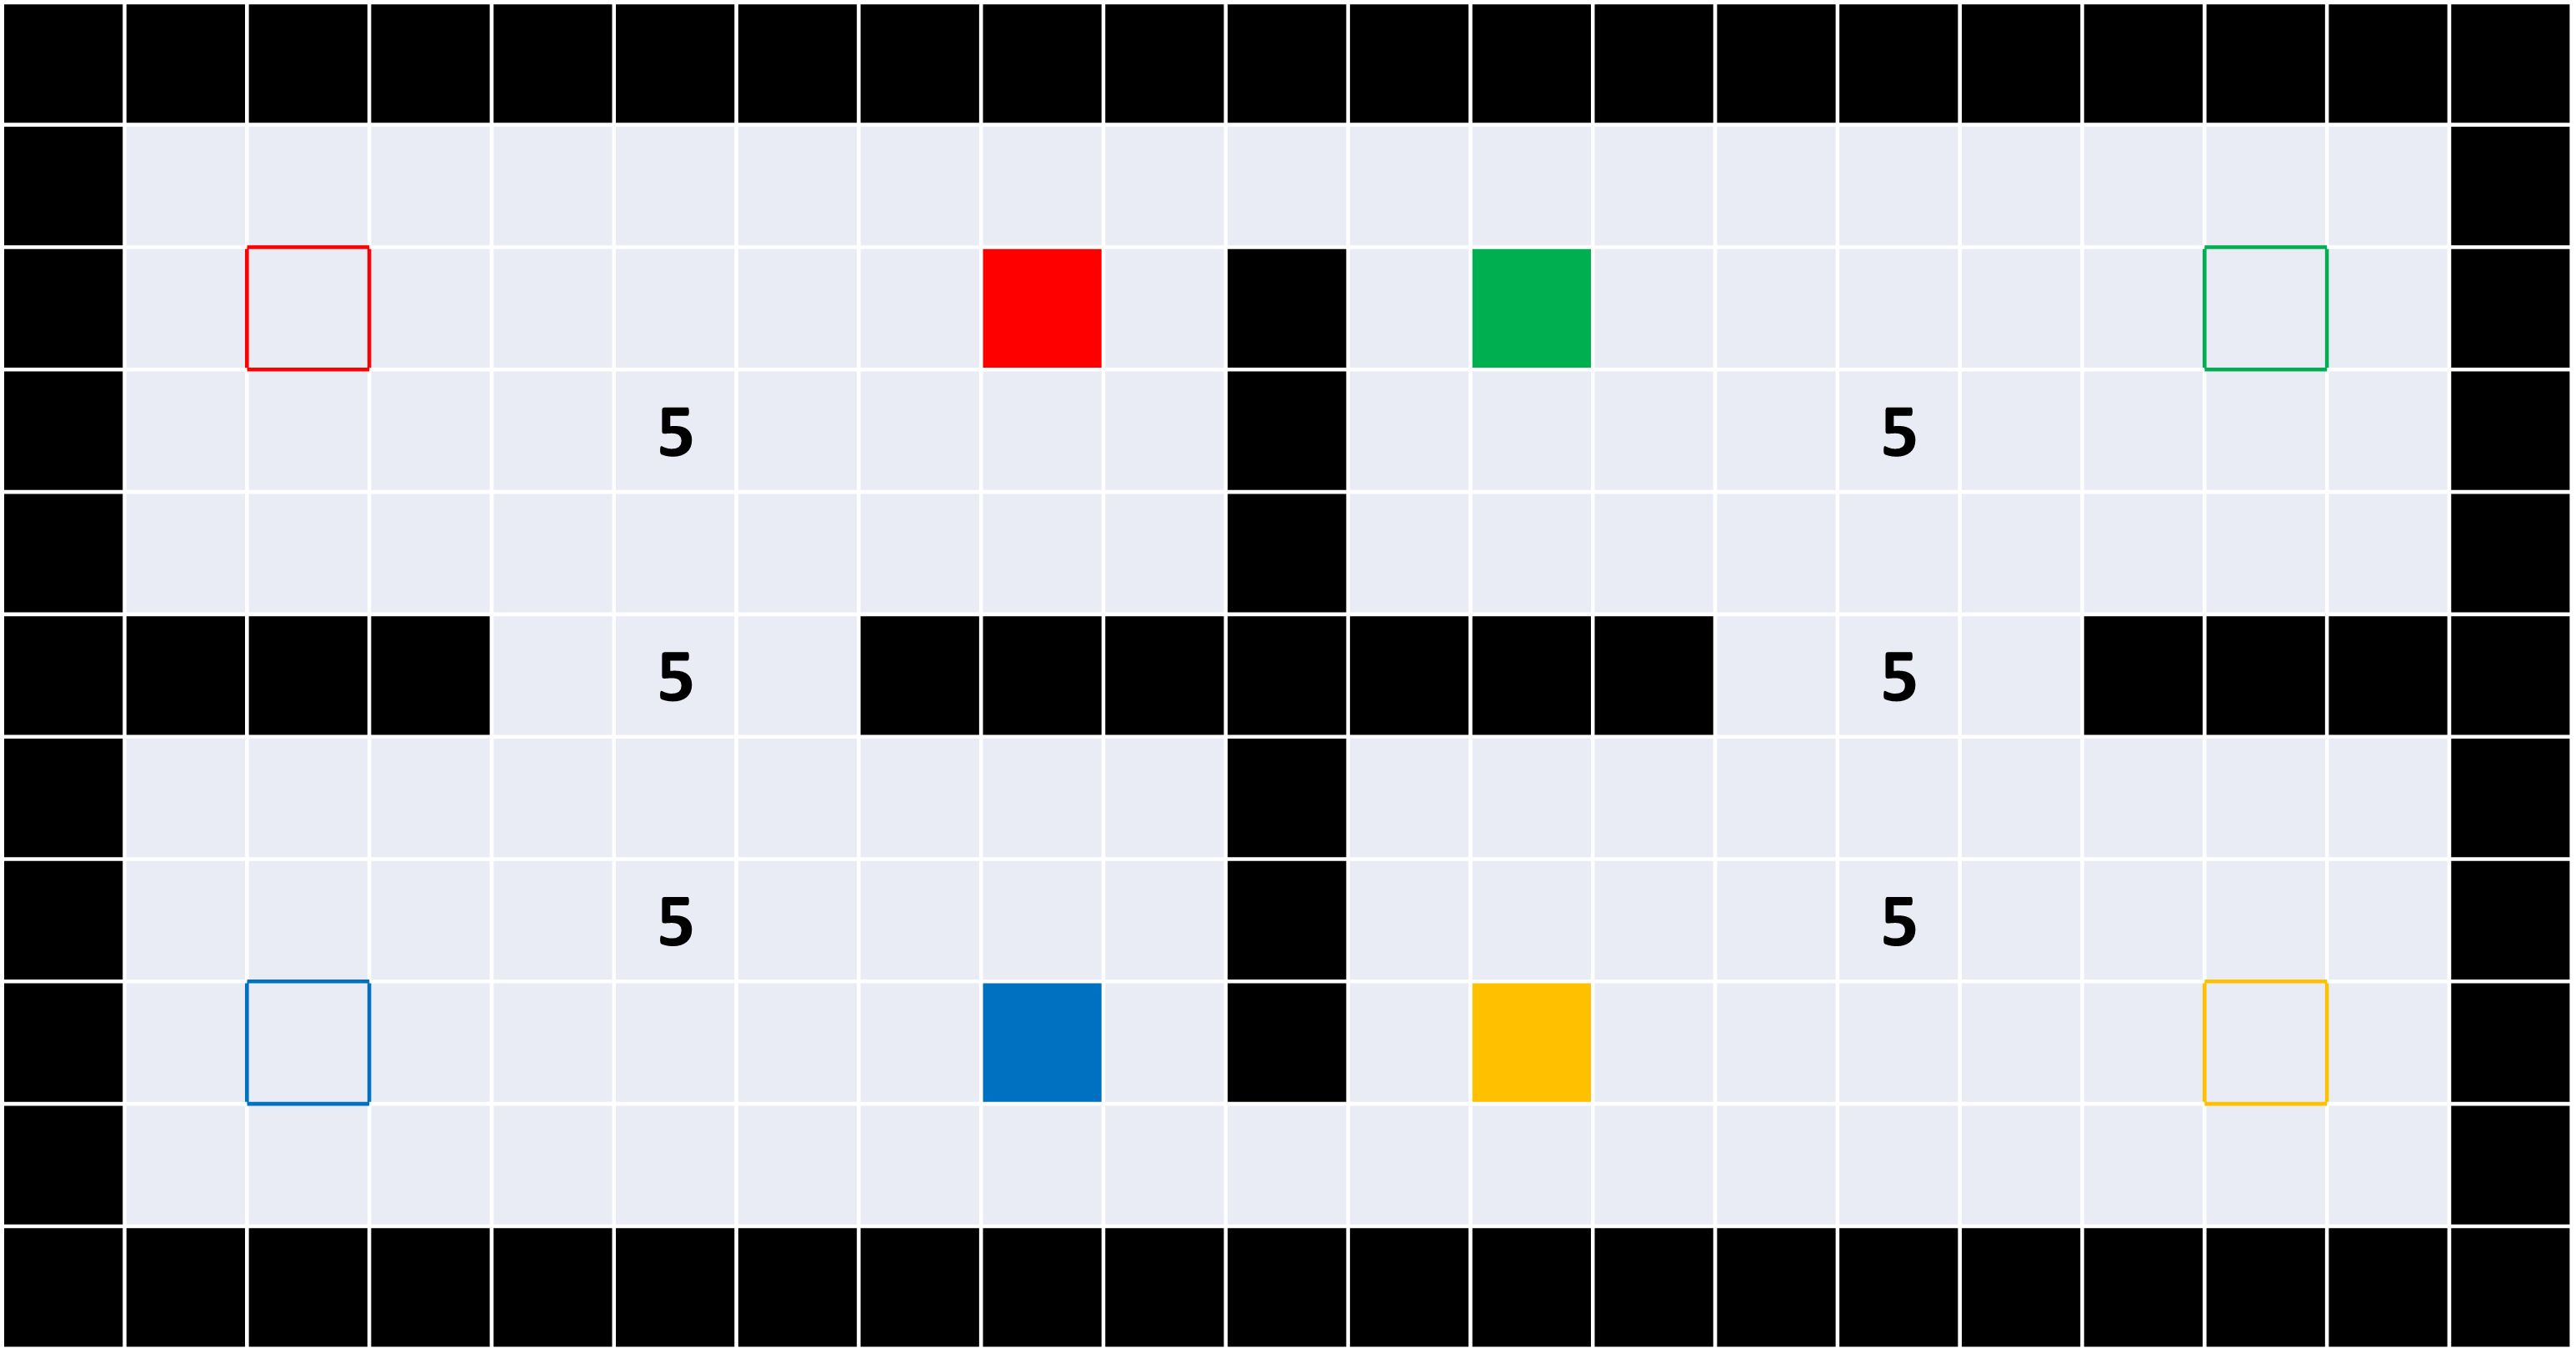
\includegraphics[width=0.27\textwidth]{Images/P2-4a.png}
%         \label{subfig:l3}} 
%     \caption{Grid SMAPF-PO benchmarks. Each color represents an agent. Initial positions are filled. Goal positions are bordered.}
%     \label{fig:multi-problems}
% \end{figure*}





% bla
% \begin{figure*}[b!]
%     \centering
%     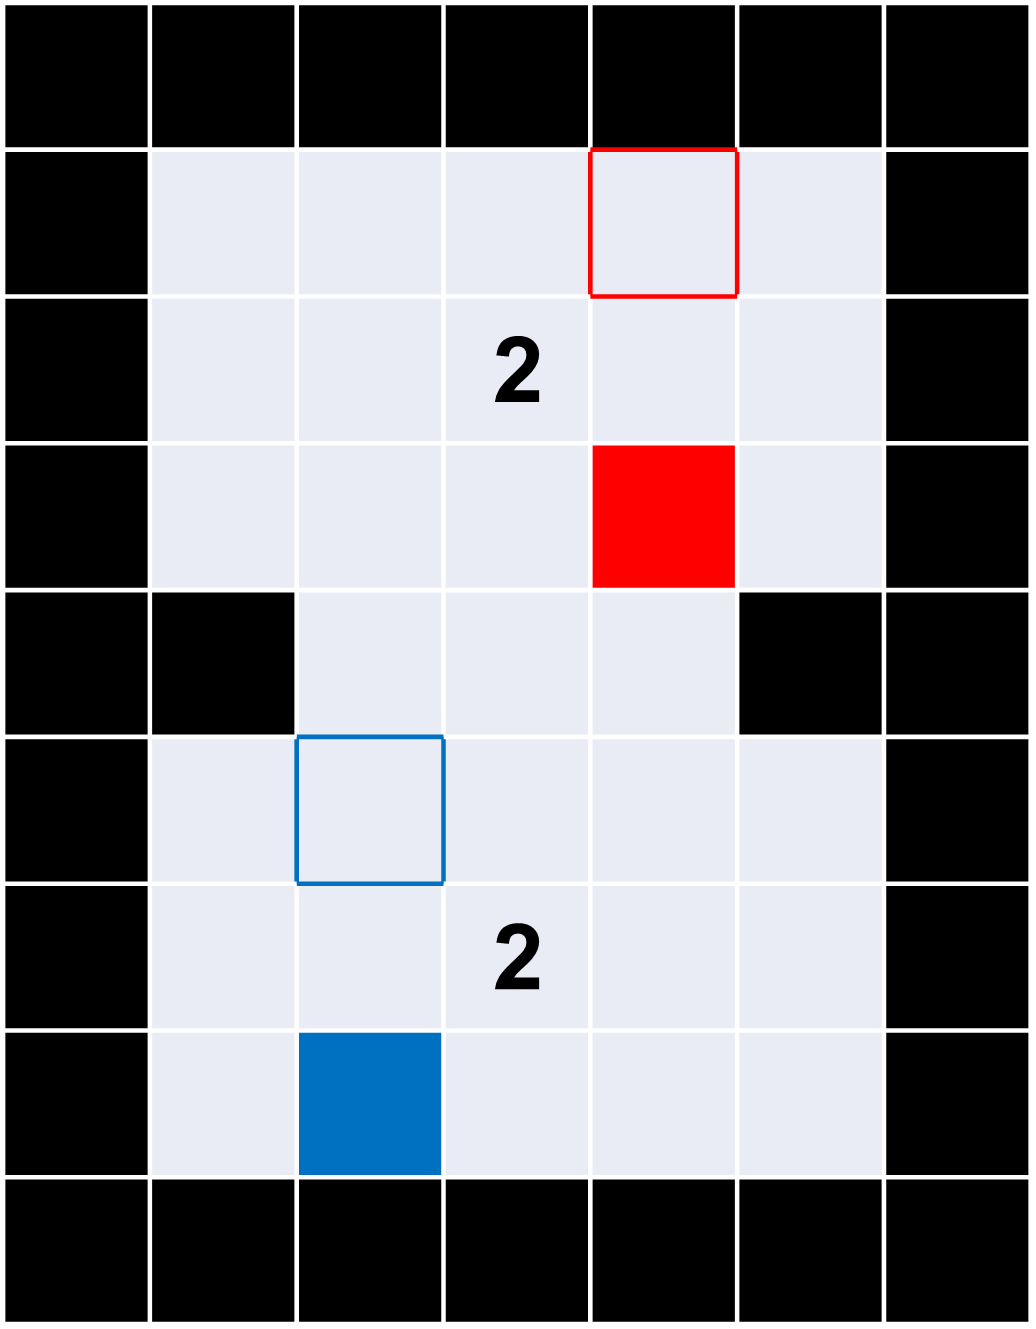
\includegraphics{Images/P1s.png}
%     \caption{Caption}
%     \label{fig:enter-label}
% \end{figure*}
% bla

% % \section{SMAPF-PO Benchmark Problems}
% \begin{figure*}[b!]
%     \subfigure[$S_1$]{
%         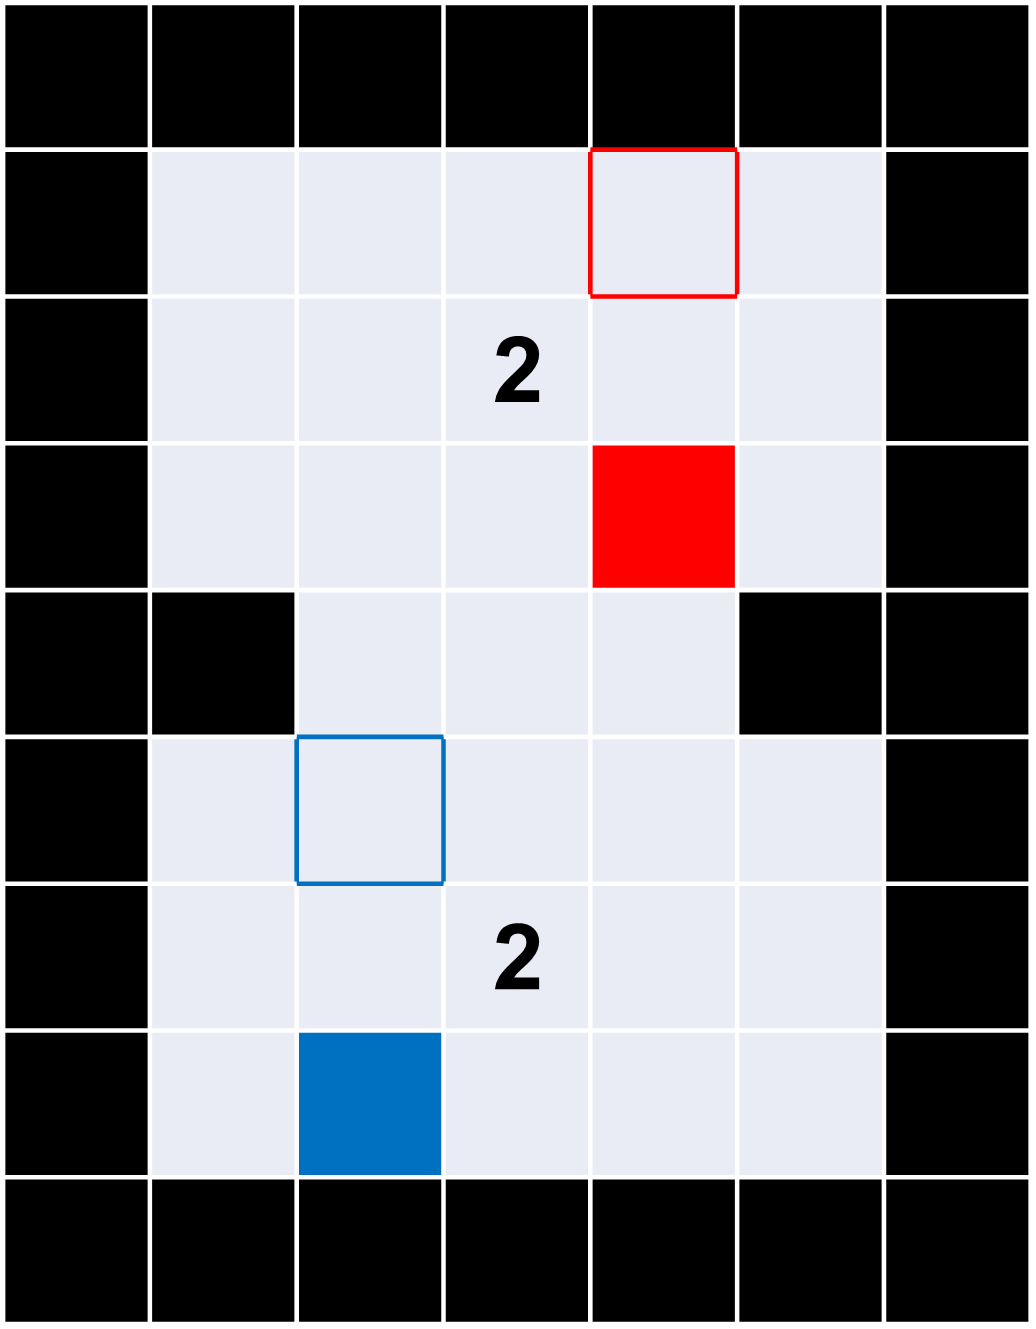
\includegraphics[width=0.1\textwidth]{Images/P1s.png}
%         \label{subfig:s1}} 
%     \subfigure[$S_2$]{
%         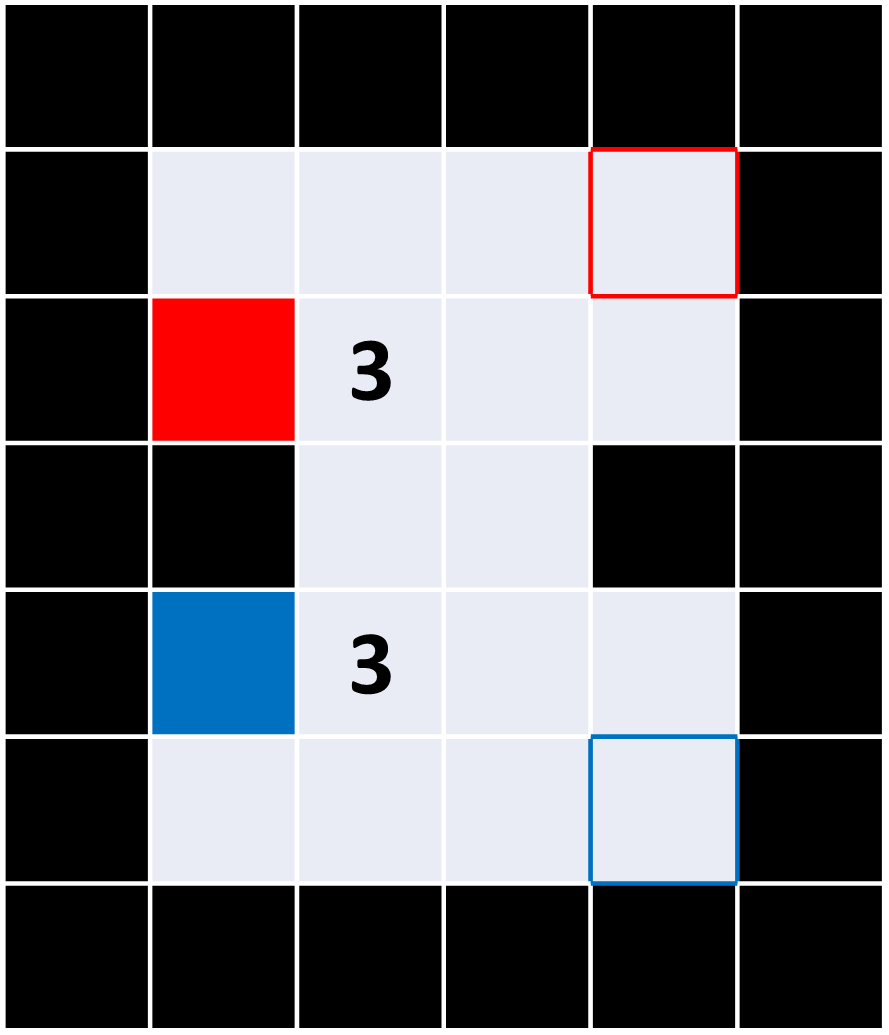
\includegraphics[width=0.11\textwidth]{Images/P2s.png}
%         \label{subfig:s2}} 
%     \subfigure[$S_3$]{
%         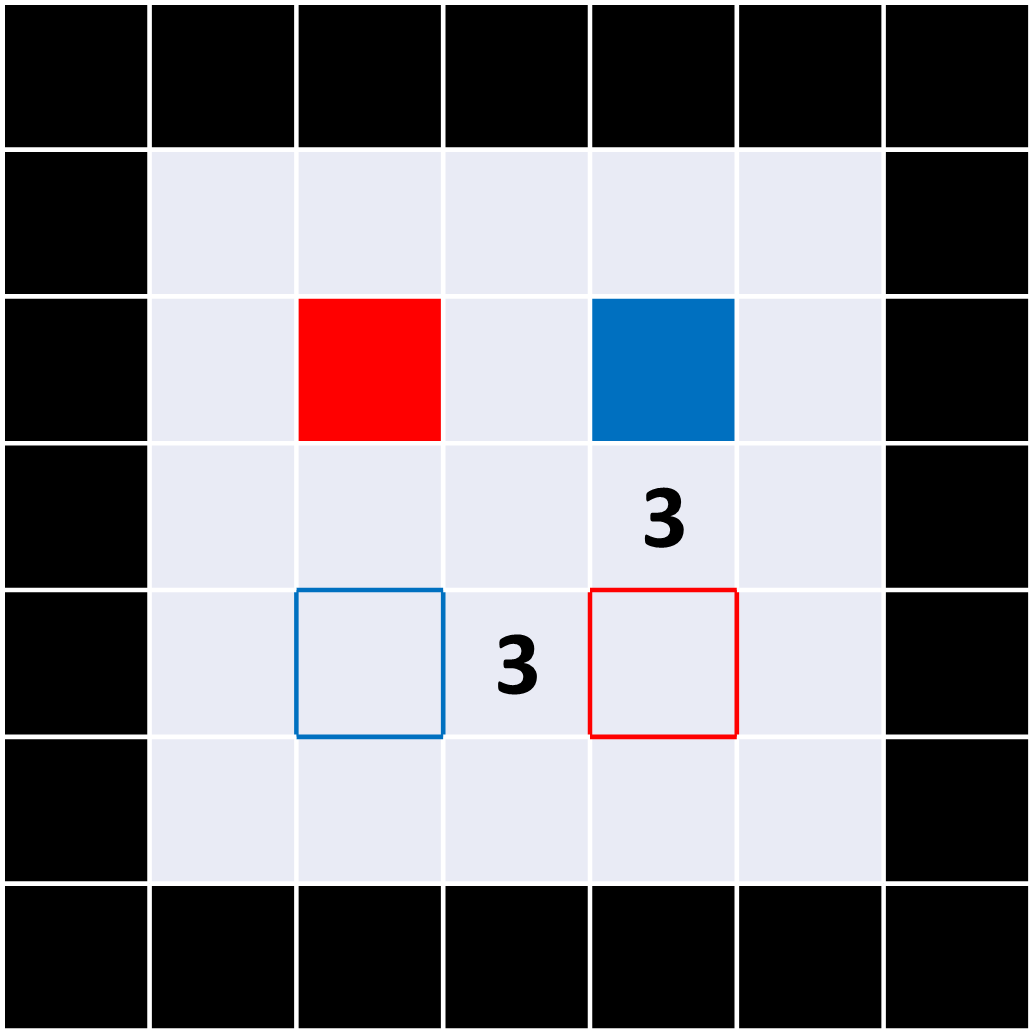
\includegraphics[width=0.13\textwidth]{Images/P3s.png}
%         \label{subfig:s3}}
%     \subfigure[$S_4$]{
%         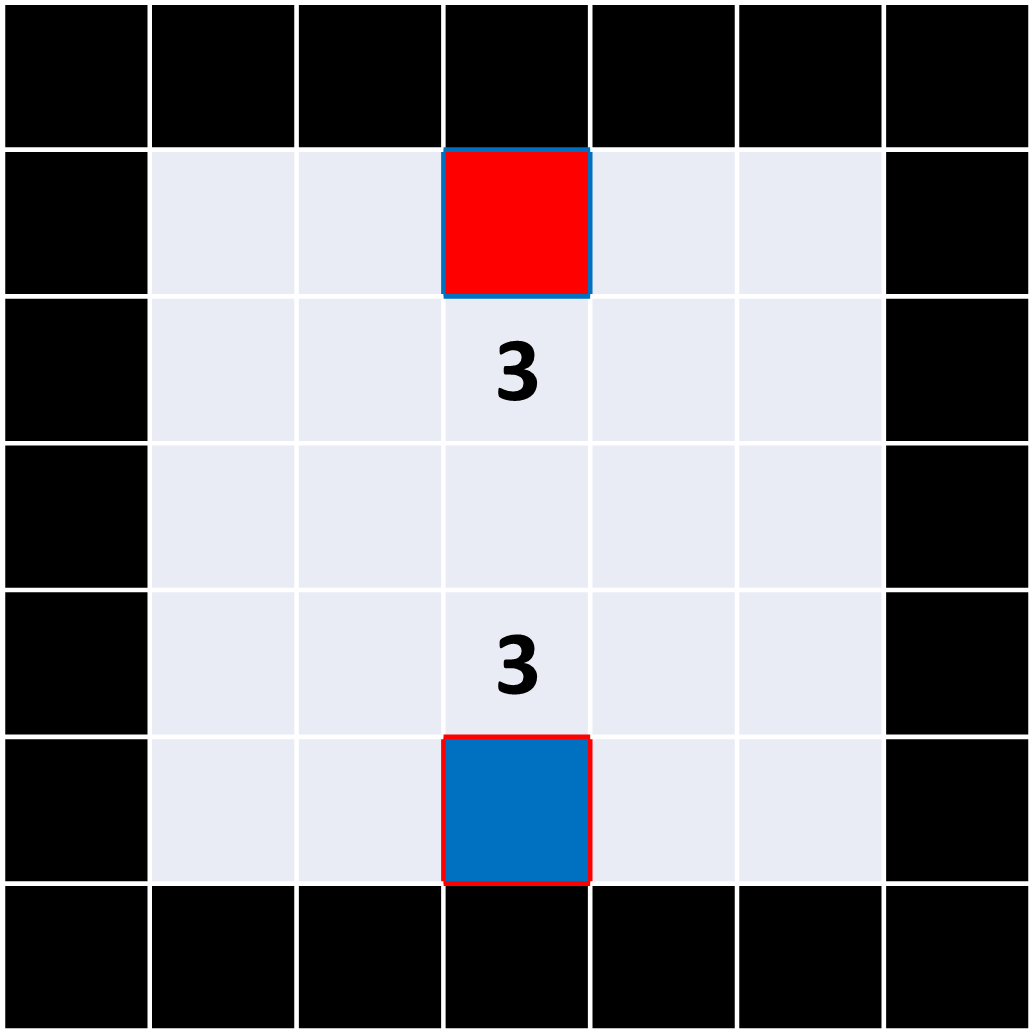
\includegraphics[width=0.13\textwidth]{Images/P4s.png}
%         \label{subfig:$S_4$}}
% %    \caption{2 agents' smaller benchmarks, used to compare our algorithm to a joint offline version.}
% %    \label{fig:small-problems}
% \subfigure[$M_1$]{
%         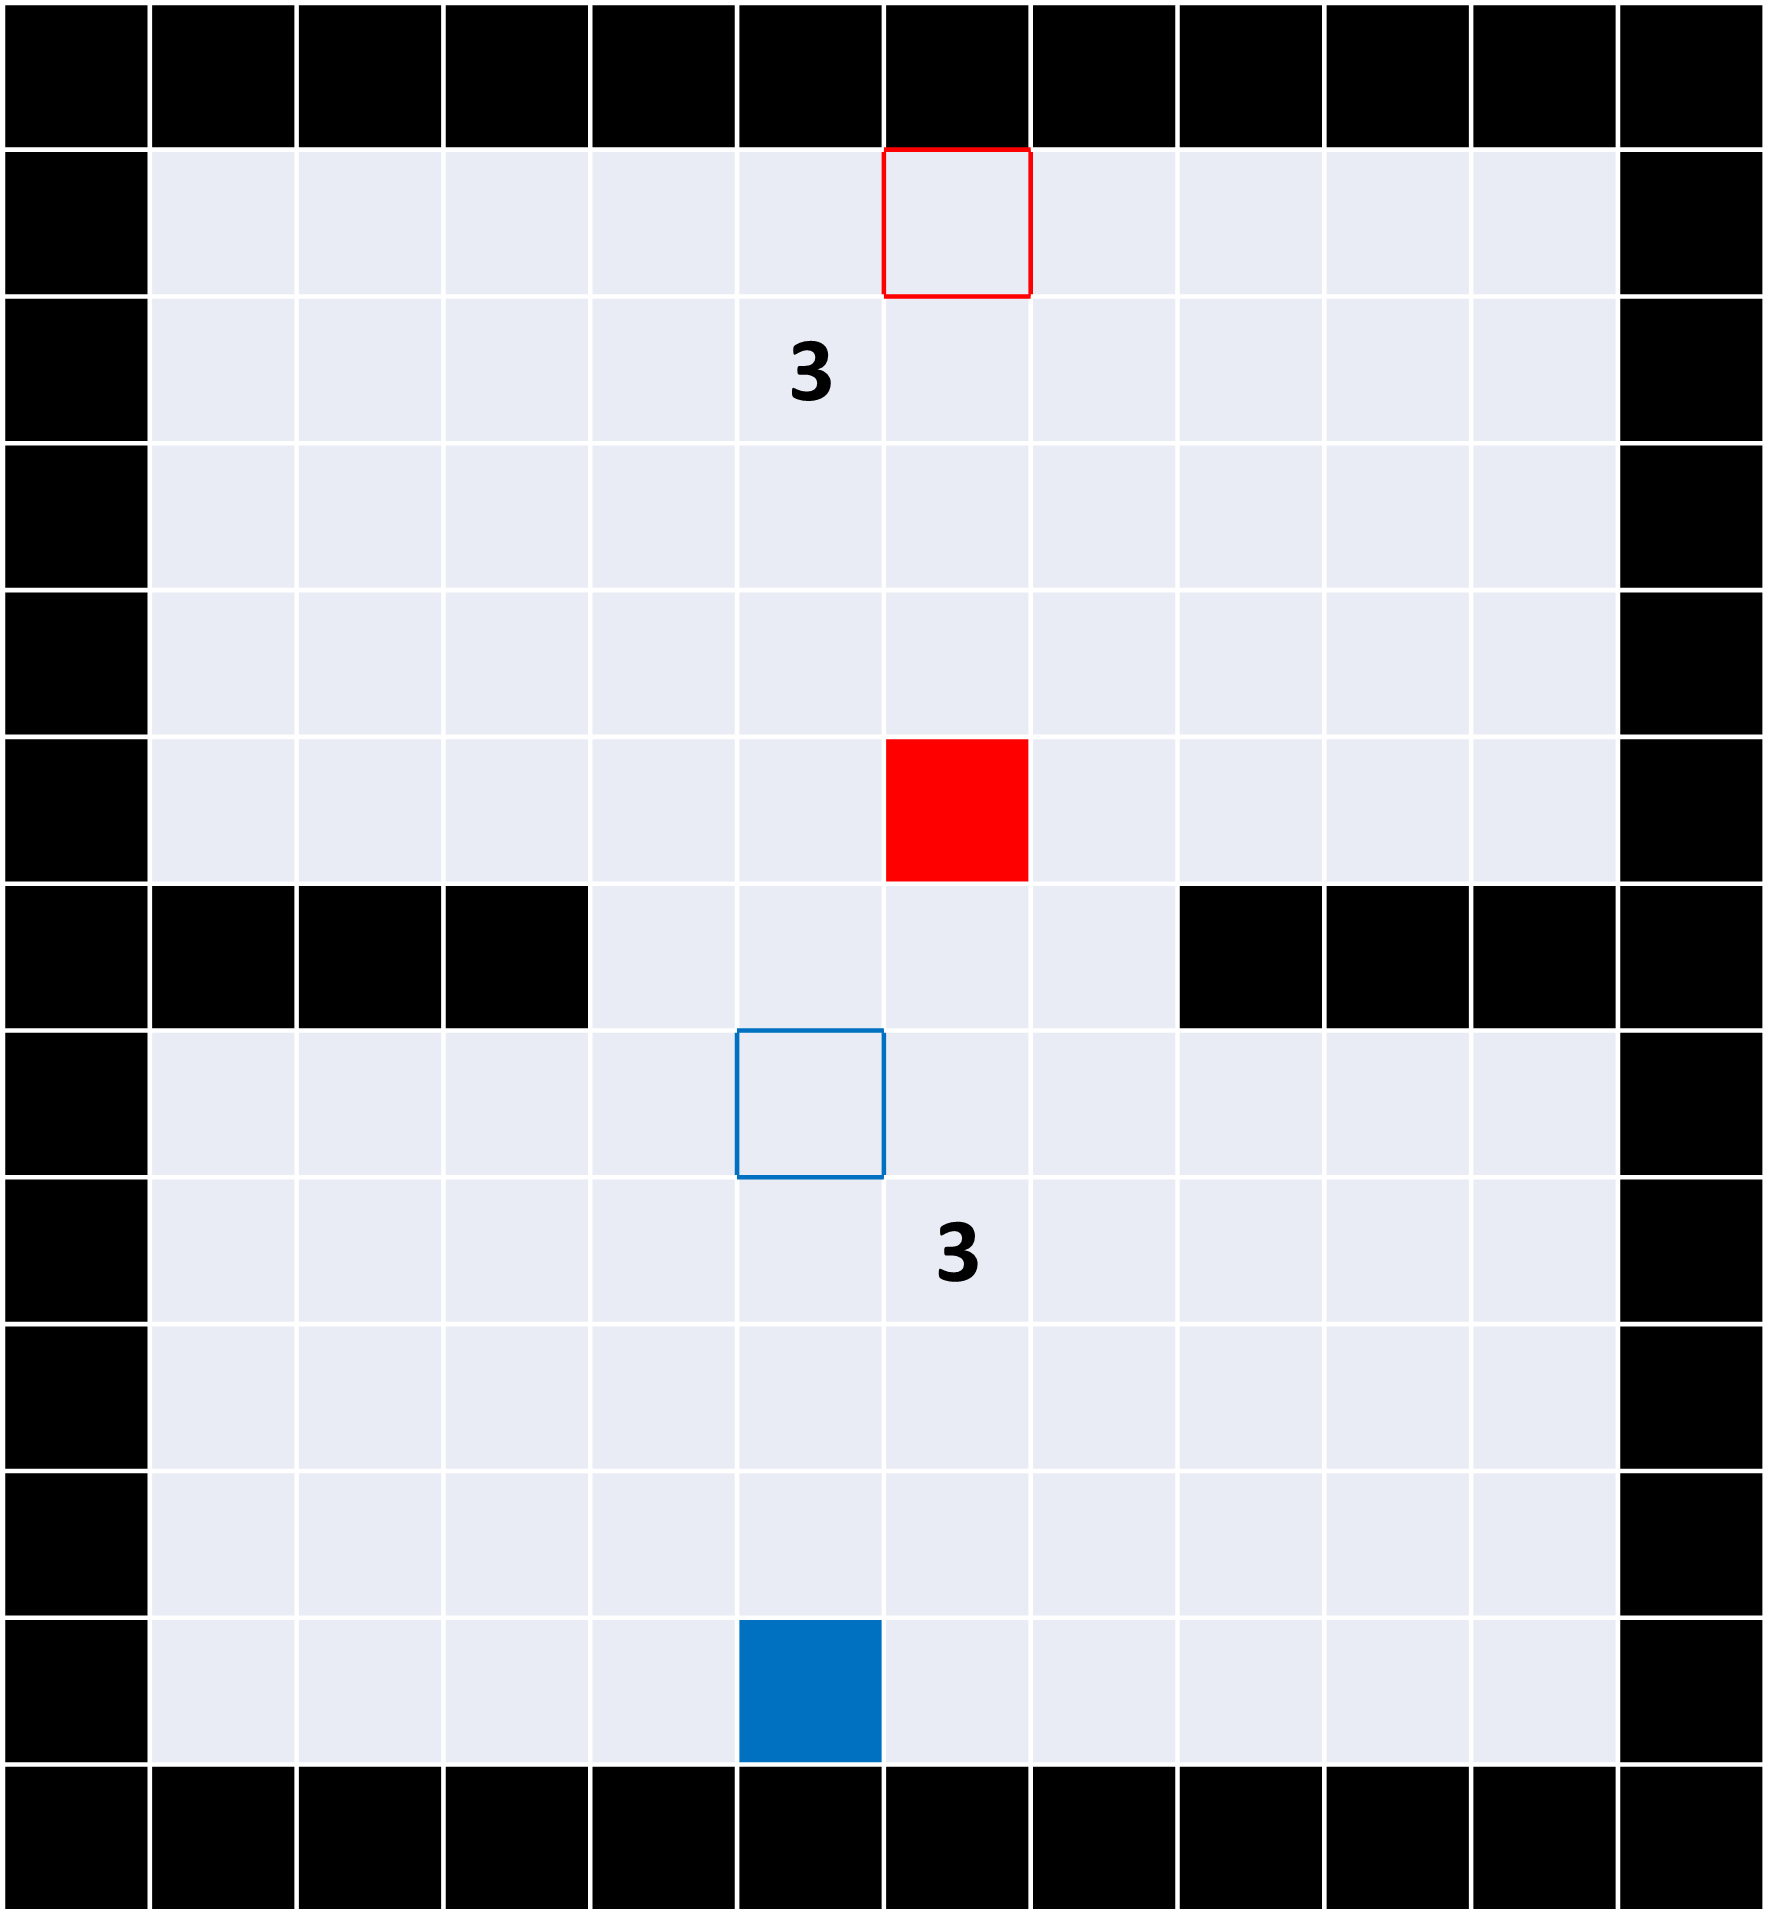
\includegraphics[width=0.12\textwidth]{Images/P1.png}
%         \label{subfig:m1}} 
%     \subfigure[$M_2$]{
%         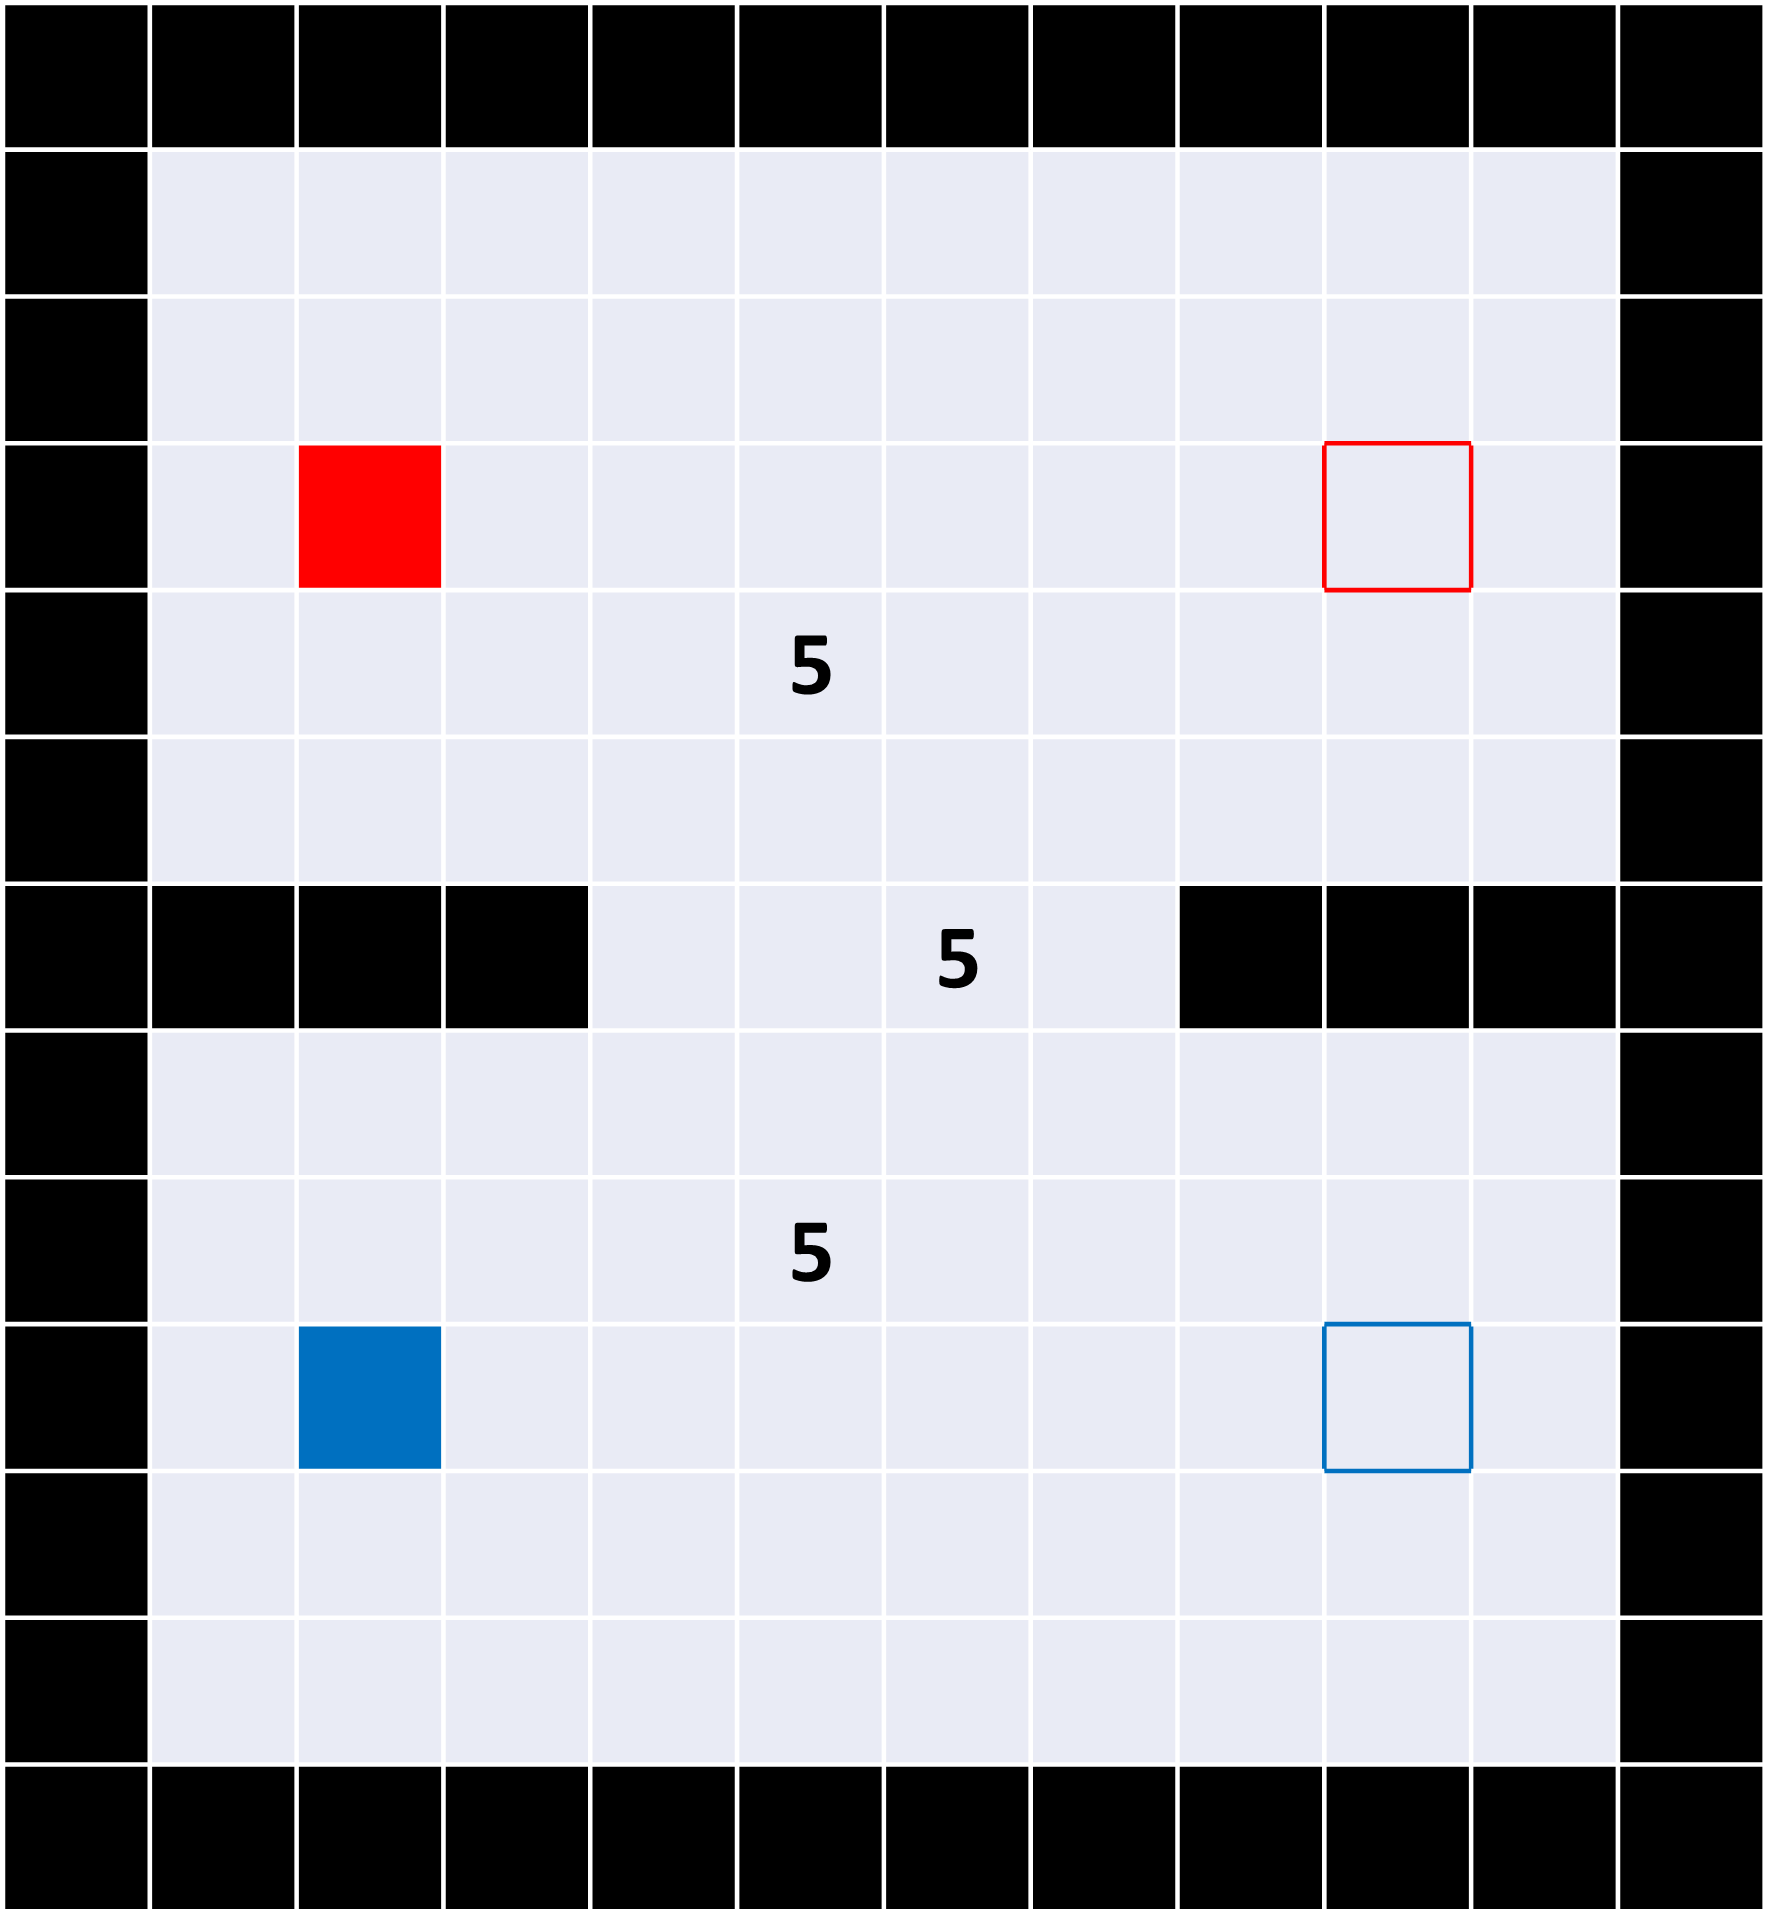
\includegraphics[width=0.12\textwidth]{Images/P2.png}
%         \label{subfig:m2}} 
%     \subfigure[$M_3$]{
%         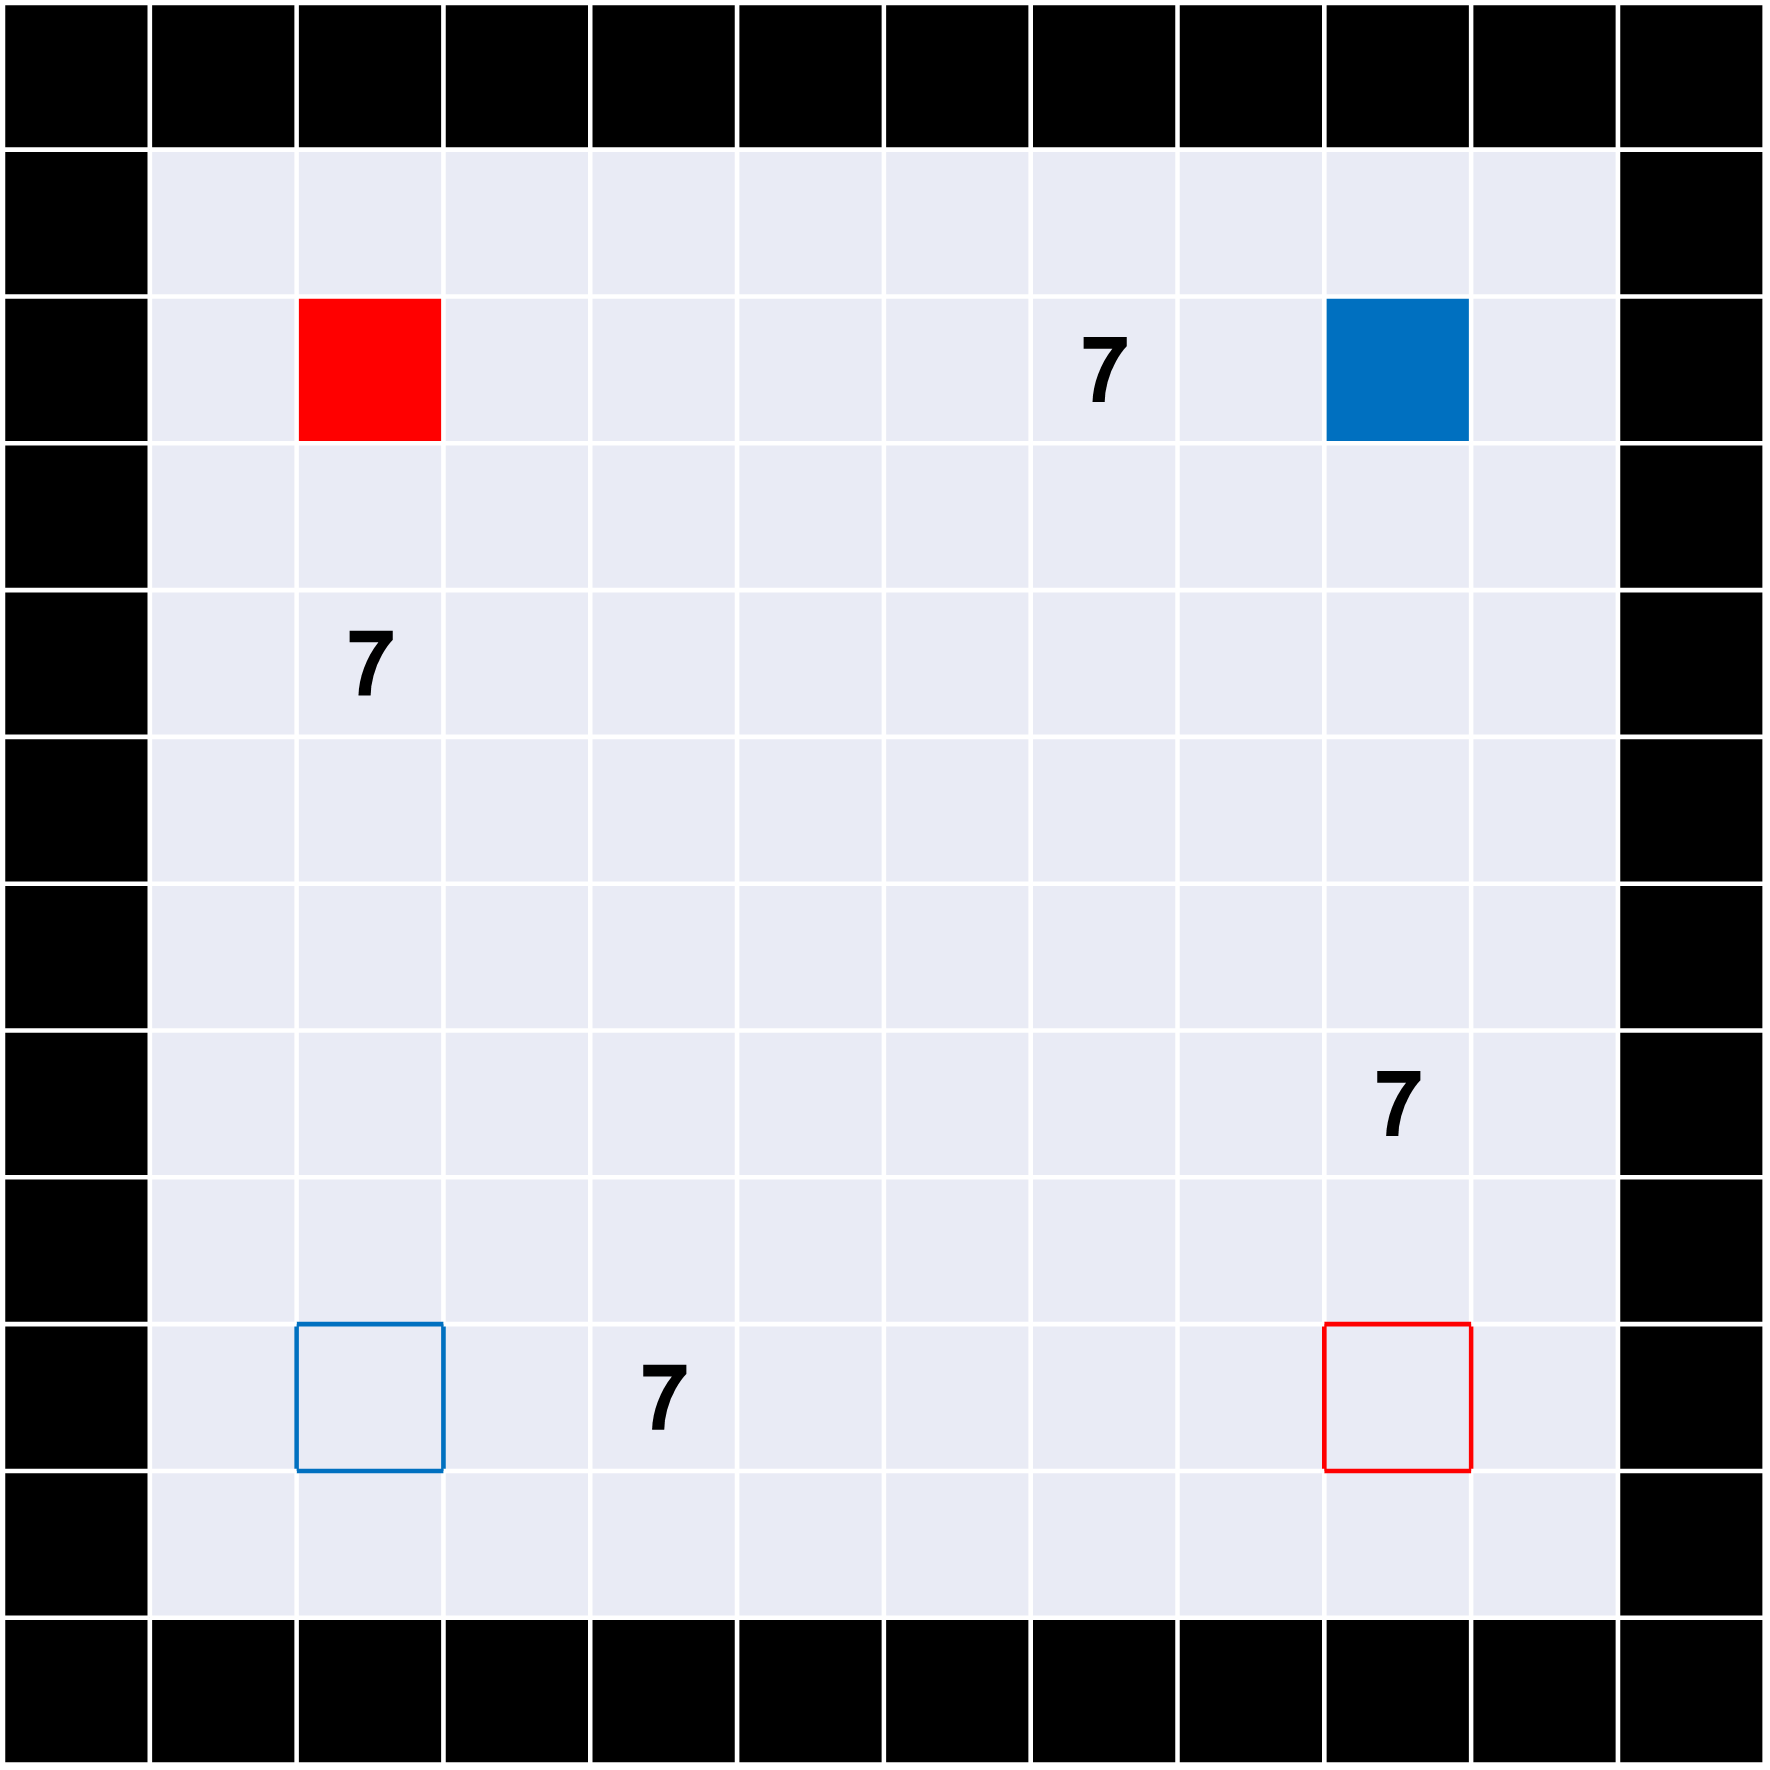
\includegraphics[width=0.13\textwidth]{Images/P3.png}
%         \label{subfig:m3}}
%     \subfigure[$M_4$]{
%         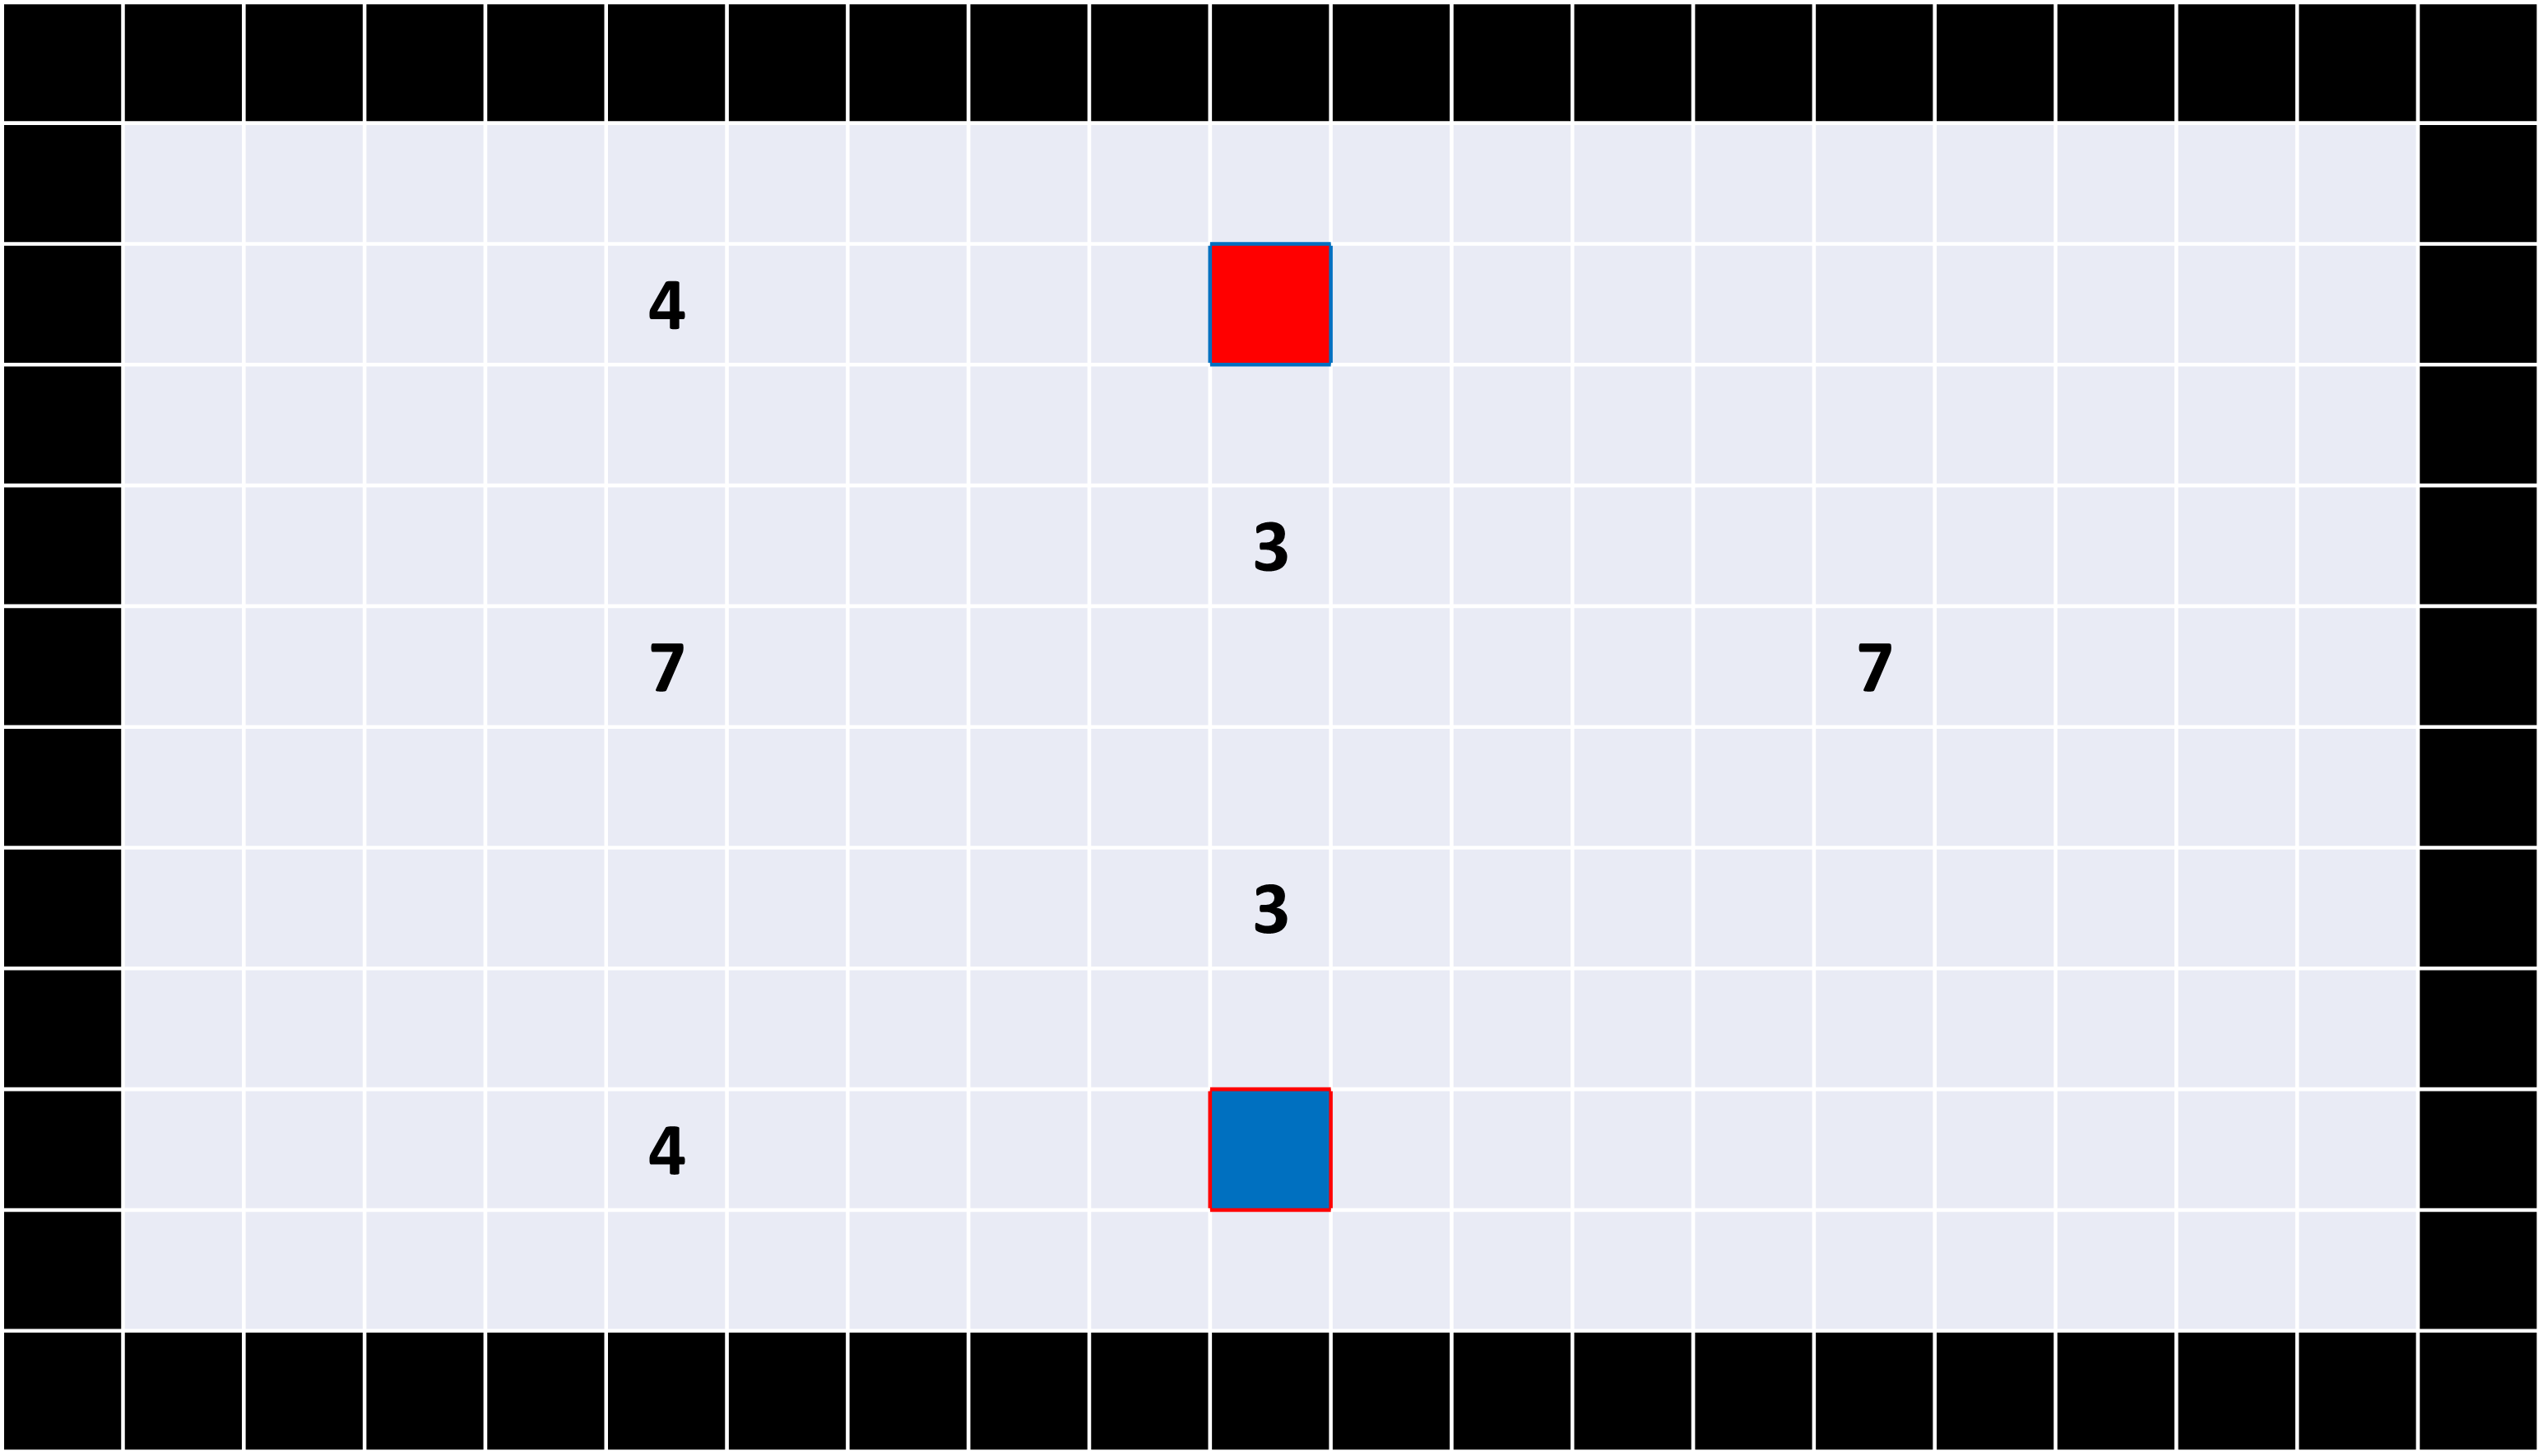
\includegraphics[width=0.245\textwidth]{Images/P4.png}
%         \label{subfig:m4}}
%     \subfigure[$M_5$]{
%         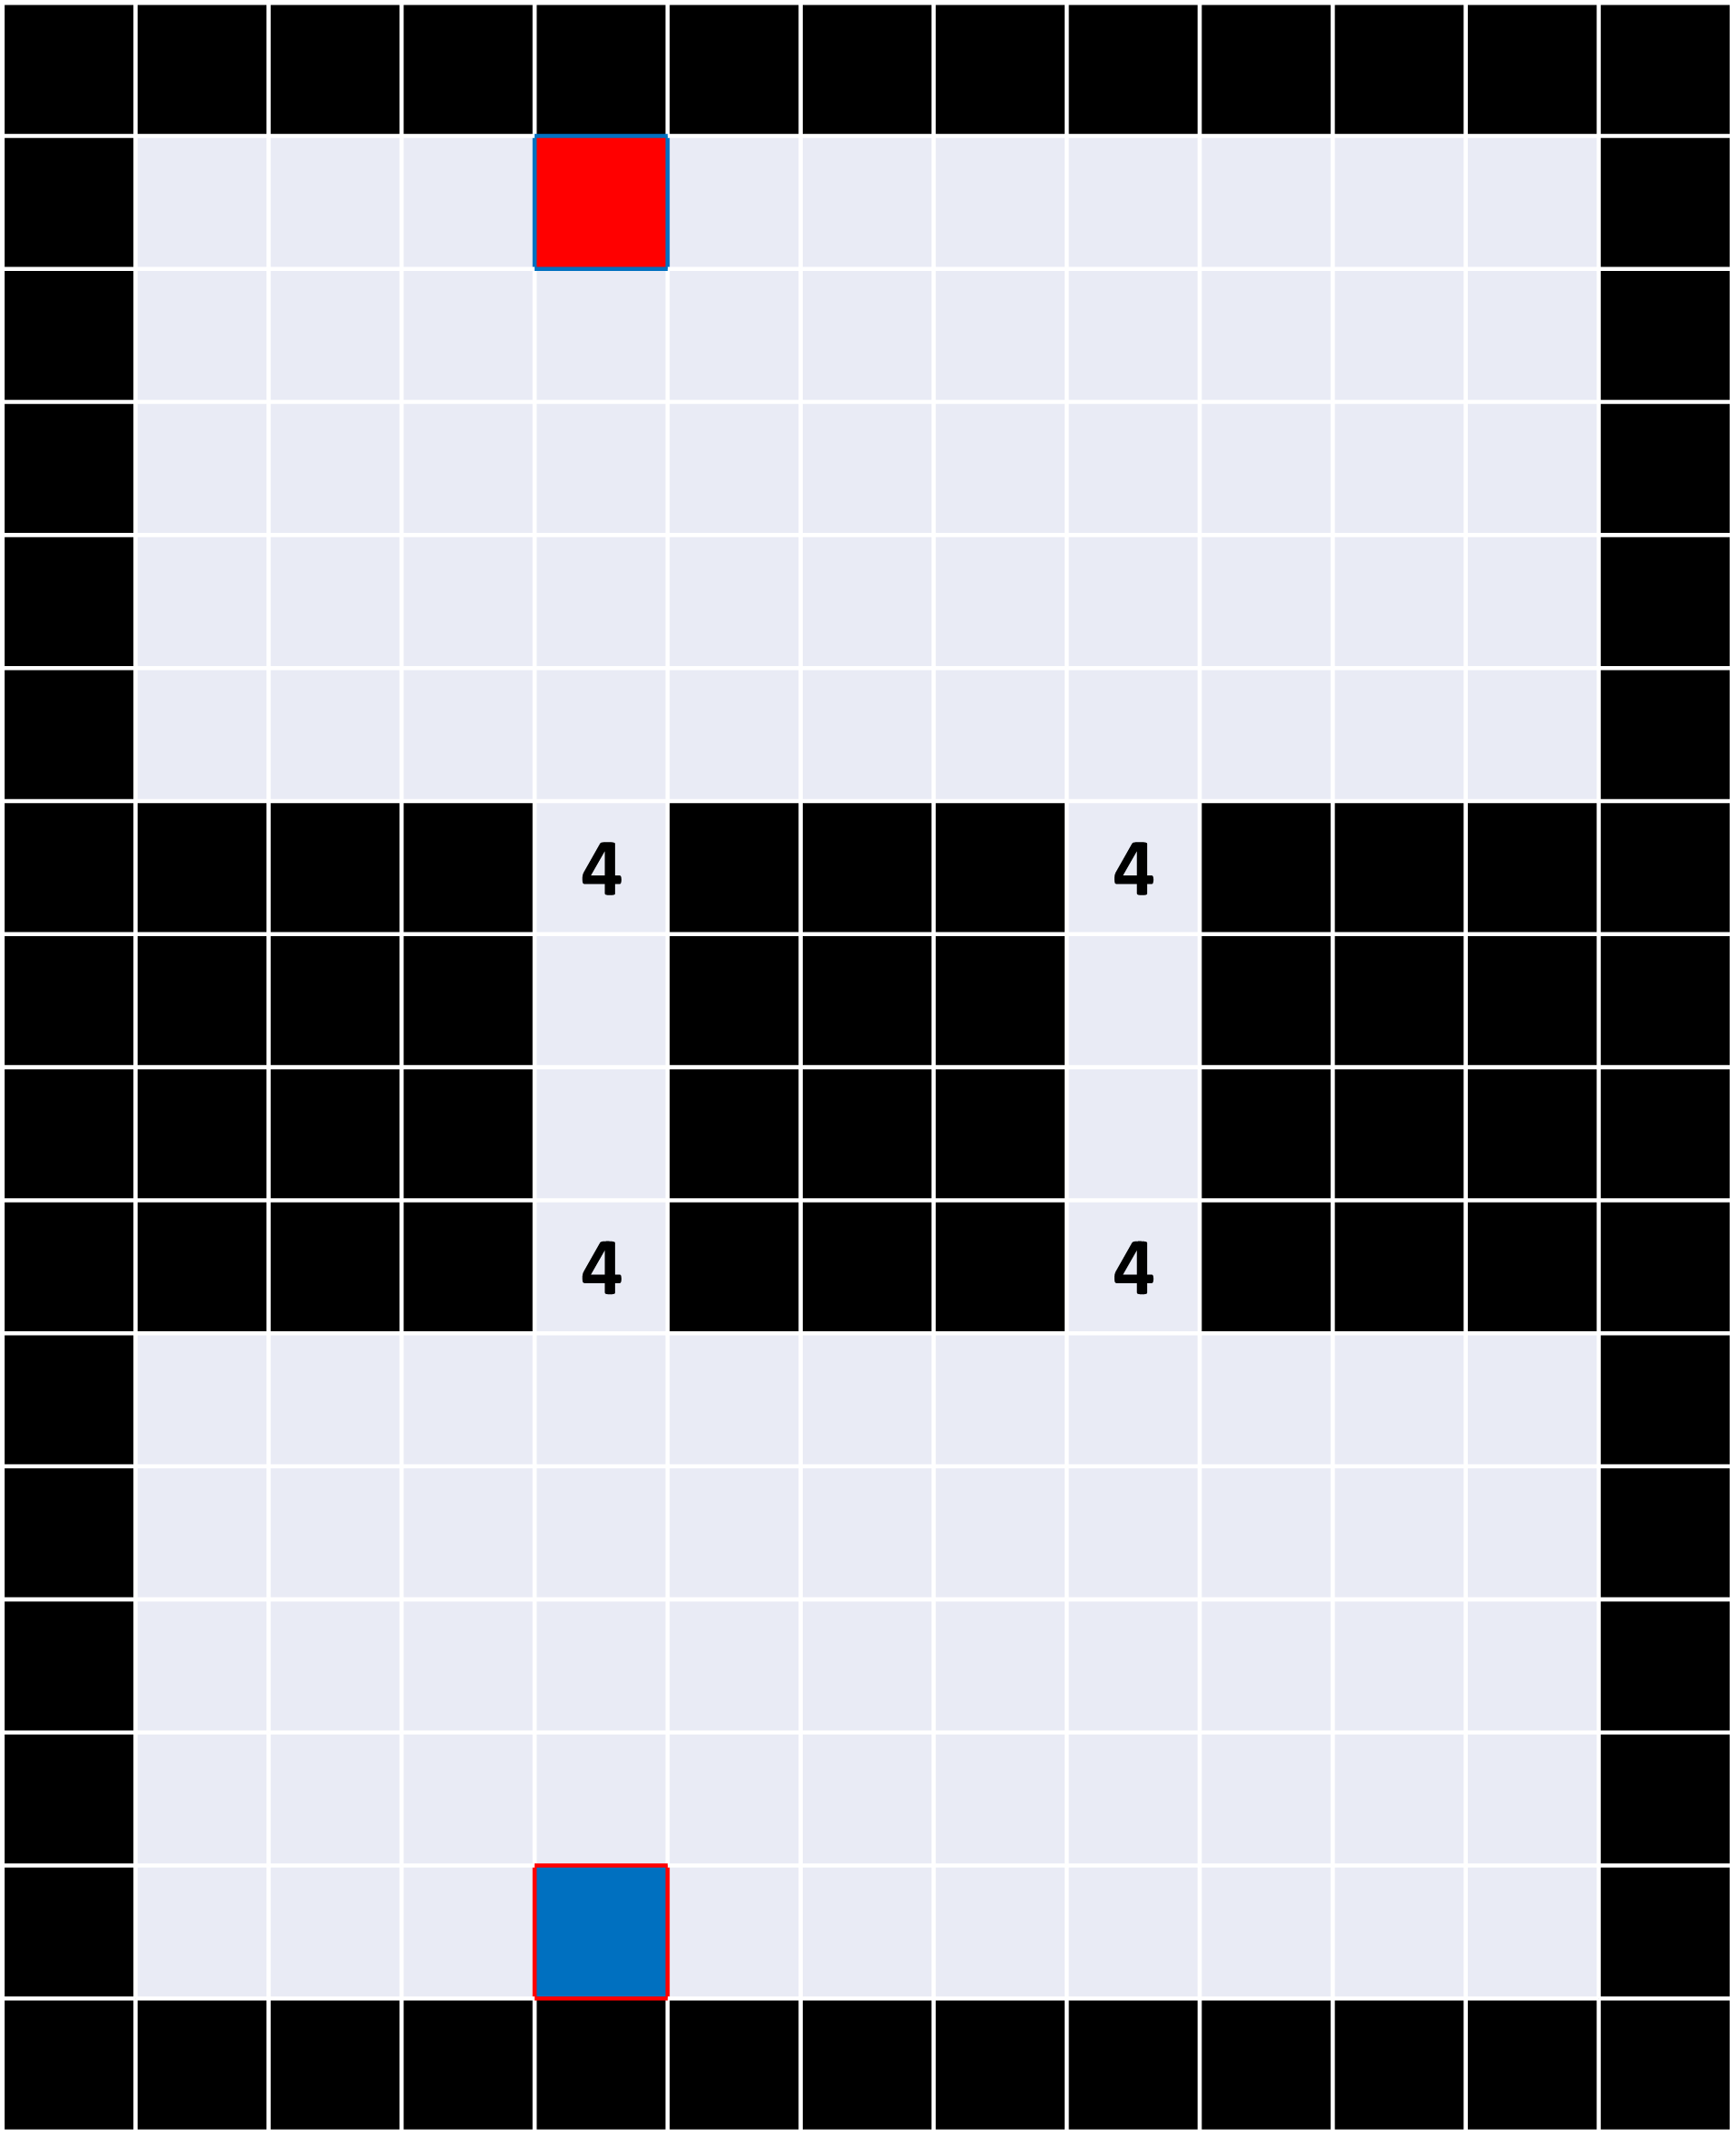
\includegraphics[width=0.115\textwidth]{Images/P5.png}
%         \label{subfig:m5}}
%     % \caption{2 agents' benchmarks used in the empirical evaluation. Each color represents an agent, where the filled cells are the agents' initial states and the bordered cells are the agents' goal states. Black cells are blocked. The numbers within cells represent beacons with respective influence range, located in those cells.}
%     % \label{fig:big-problems}
%      \subfigure[$L_1$]{
%         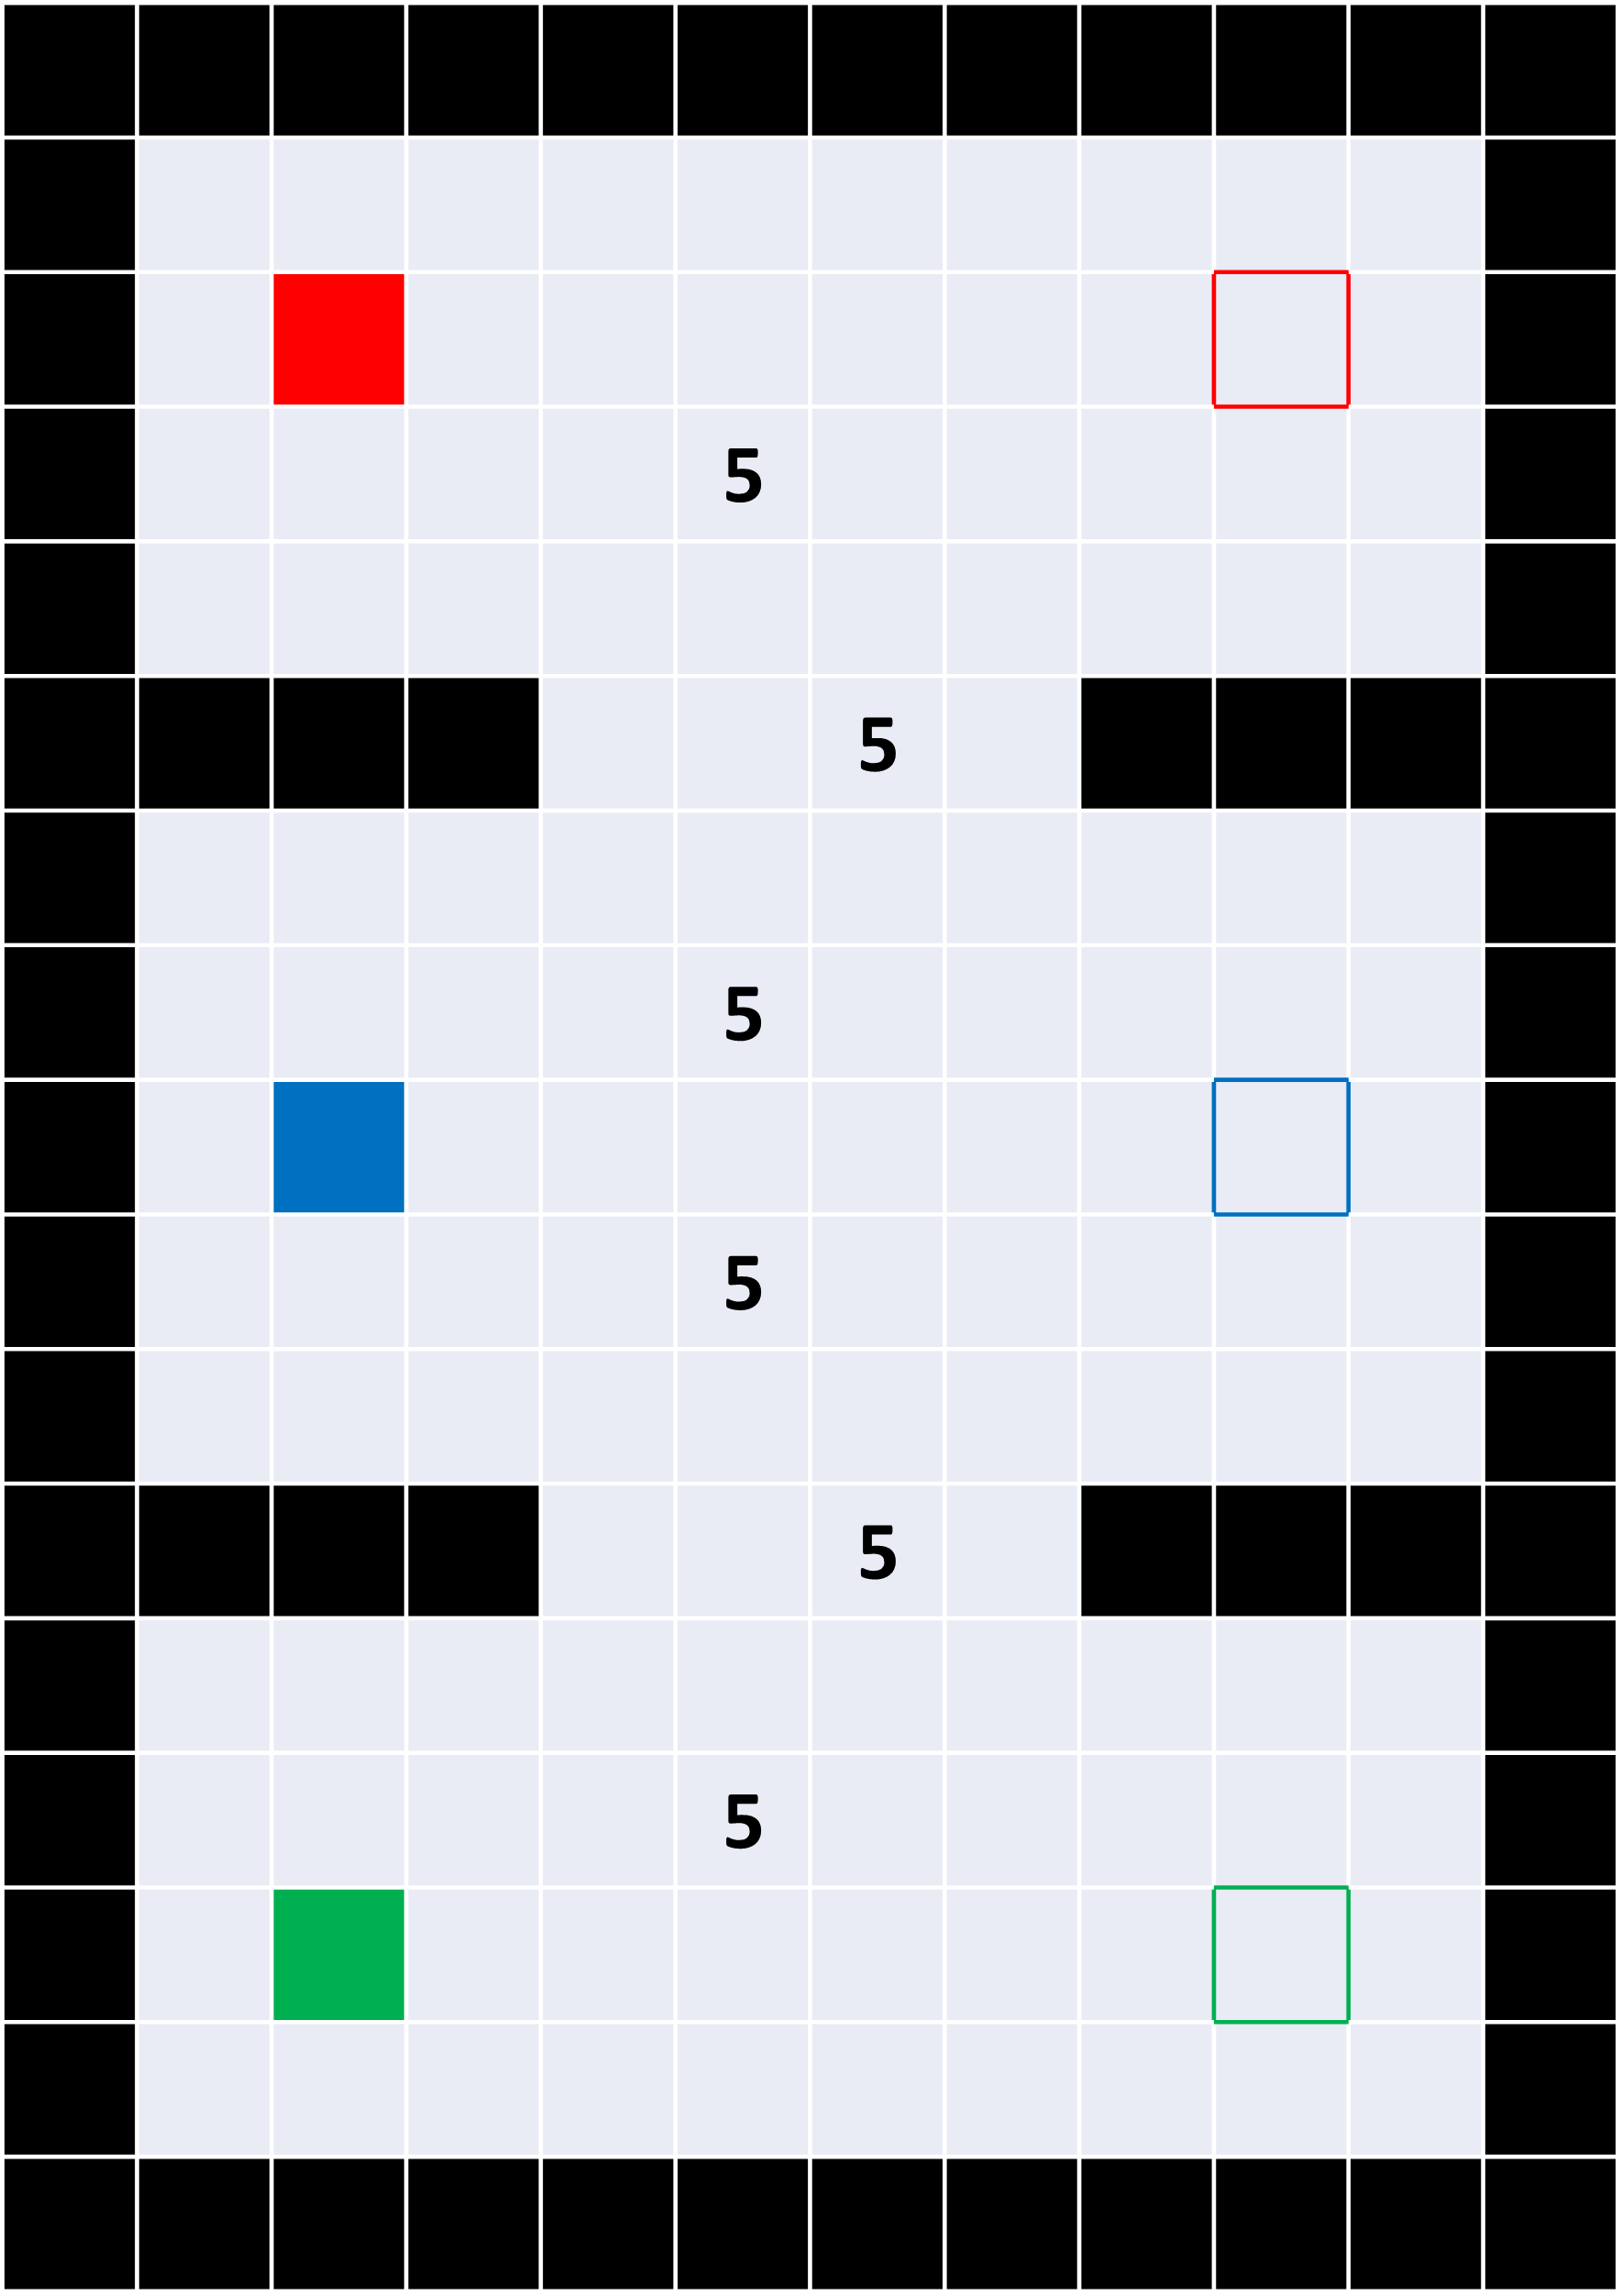
\includegraphics[width=0.1\textwidth]{Images/P2-3a.png}
%         \label{subfig:l1}}
%     \subfigure[$L_2$]{
%         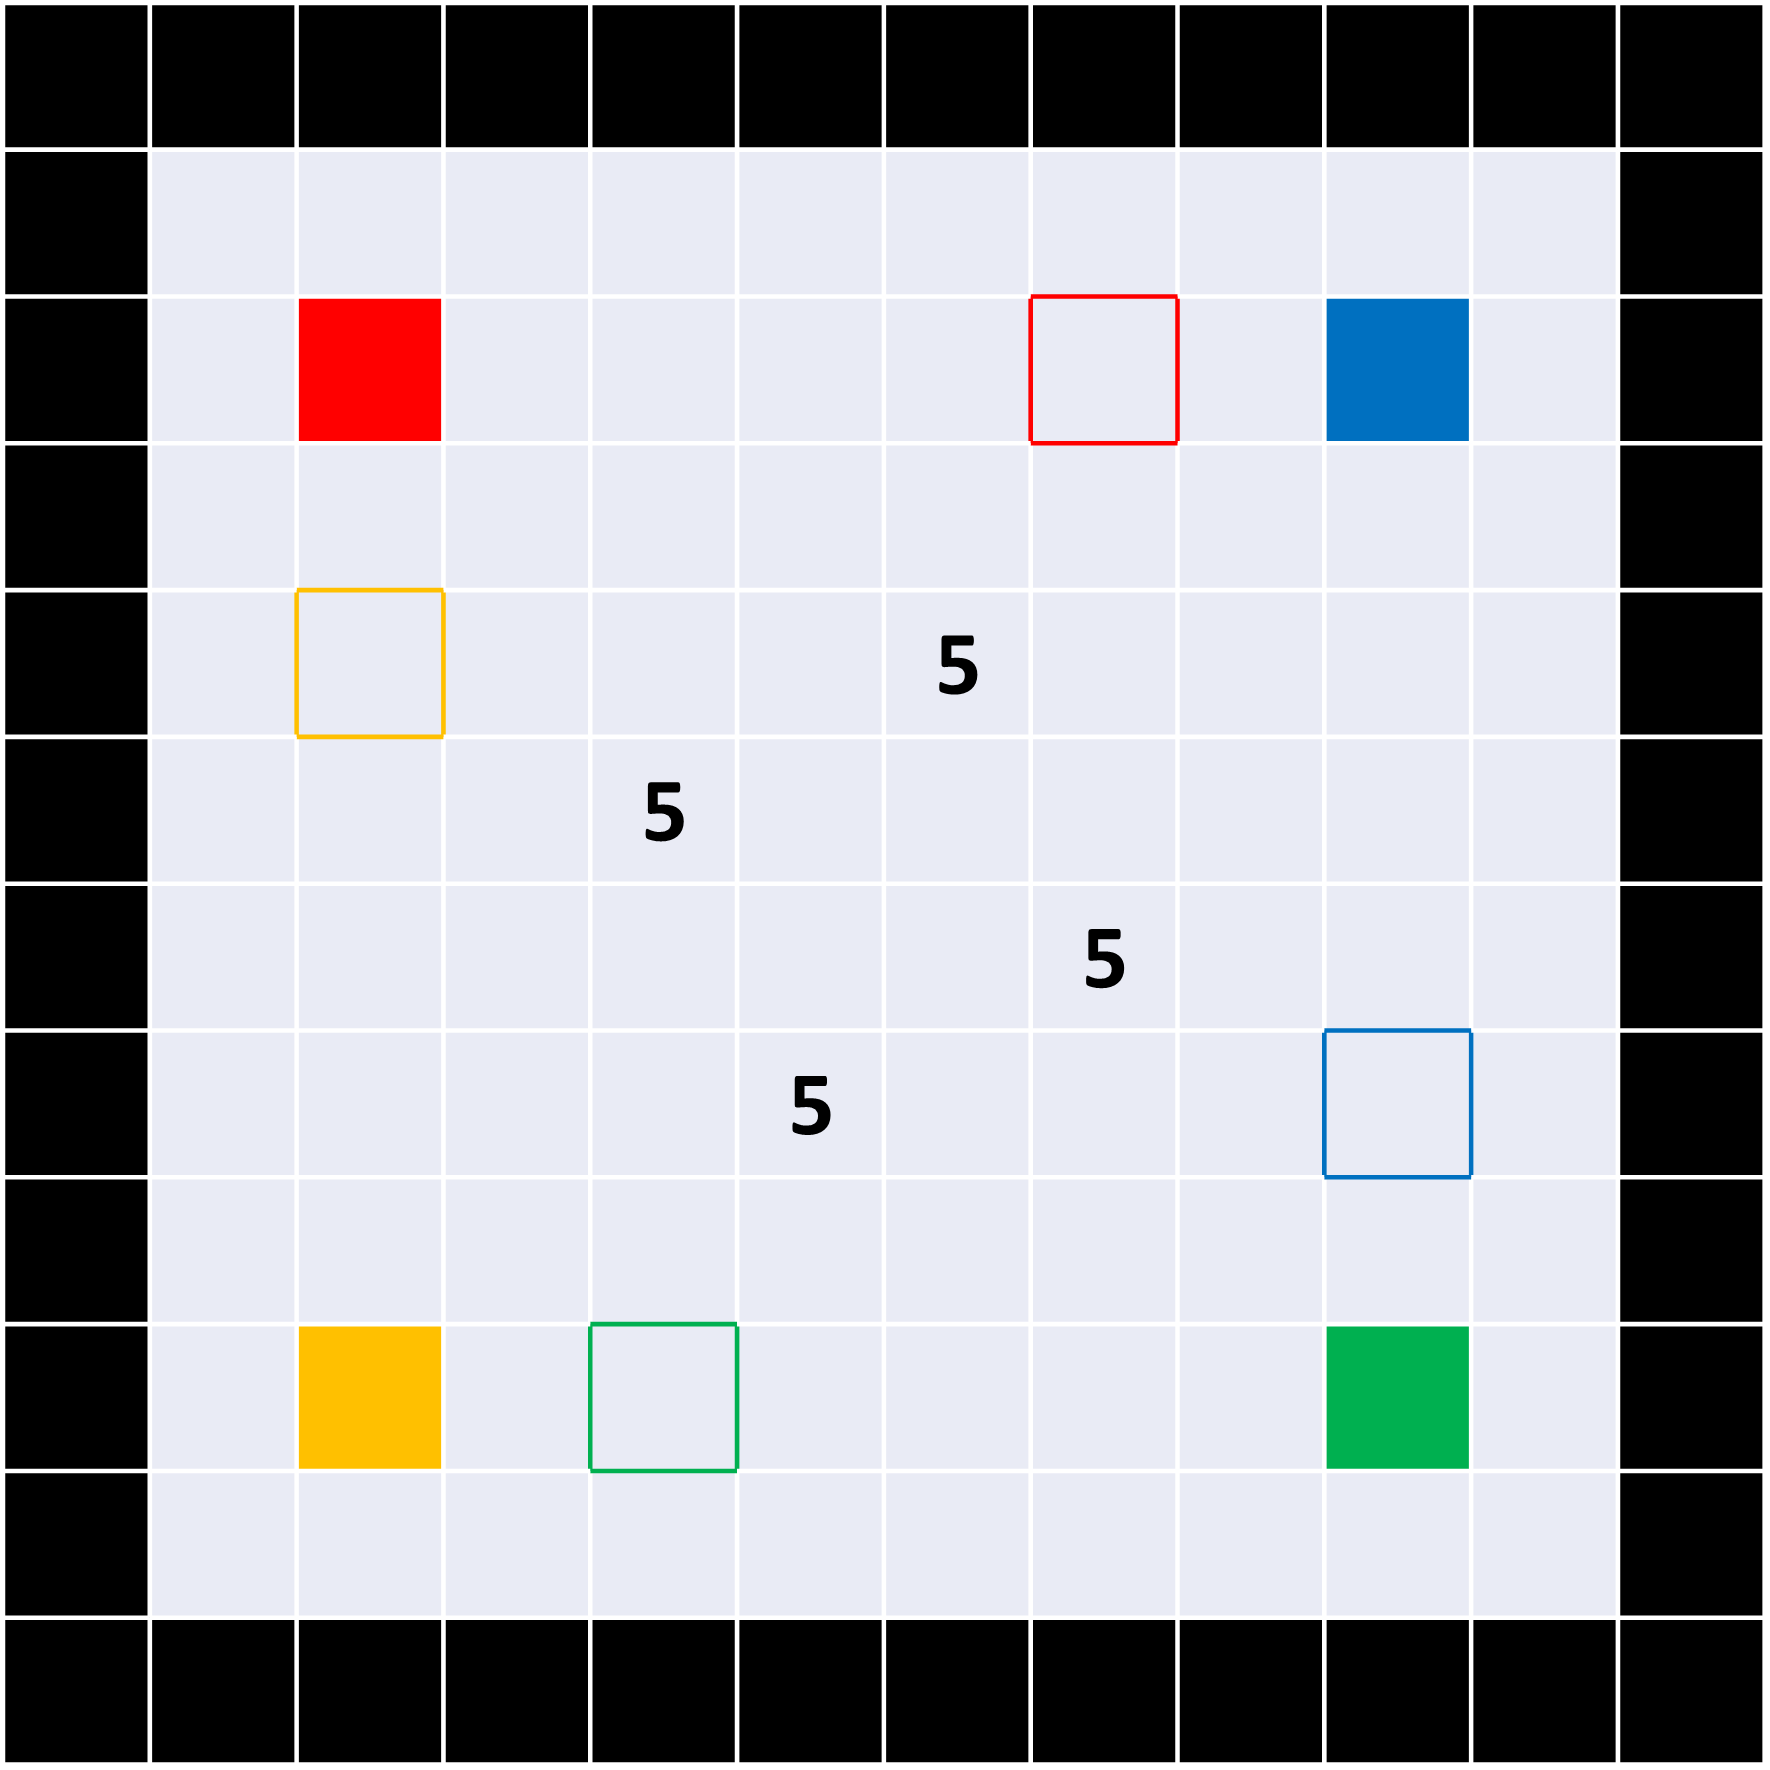
\includegraphics[width=0.1425\textwidth]{Images/P3-4a.png}
%         \label{subfig:l2}}
%     \subfigure[$L_3$]{
%         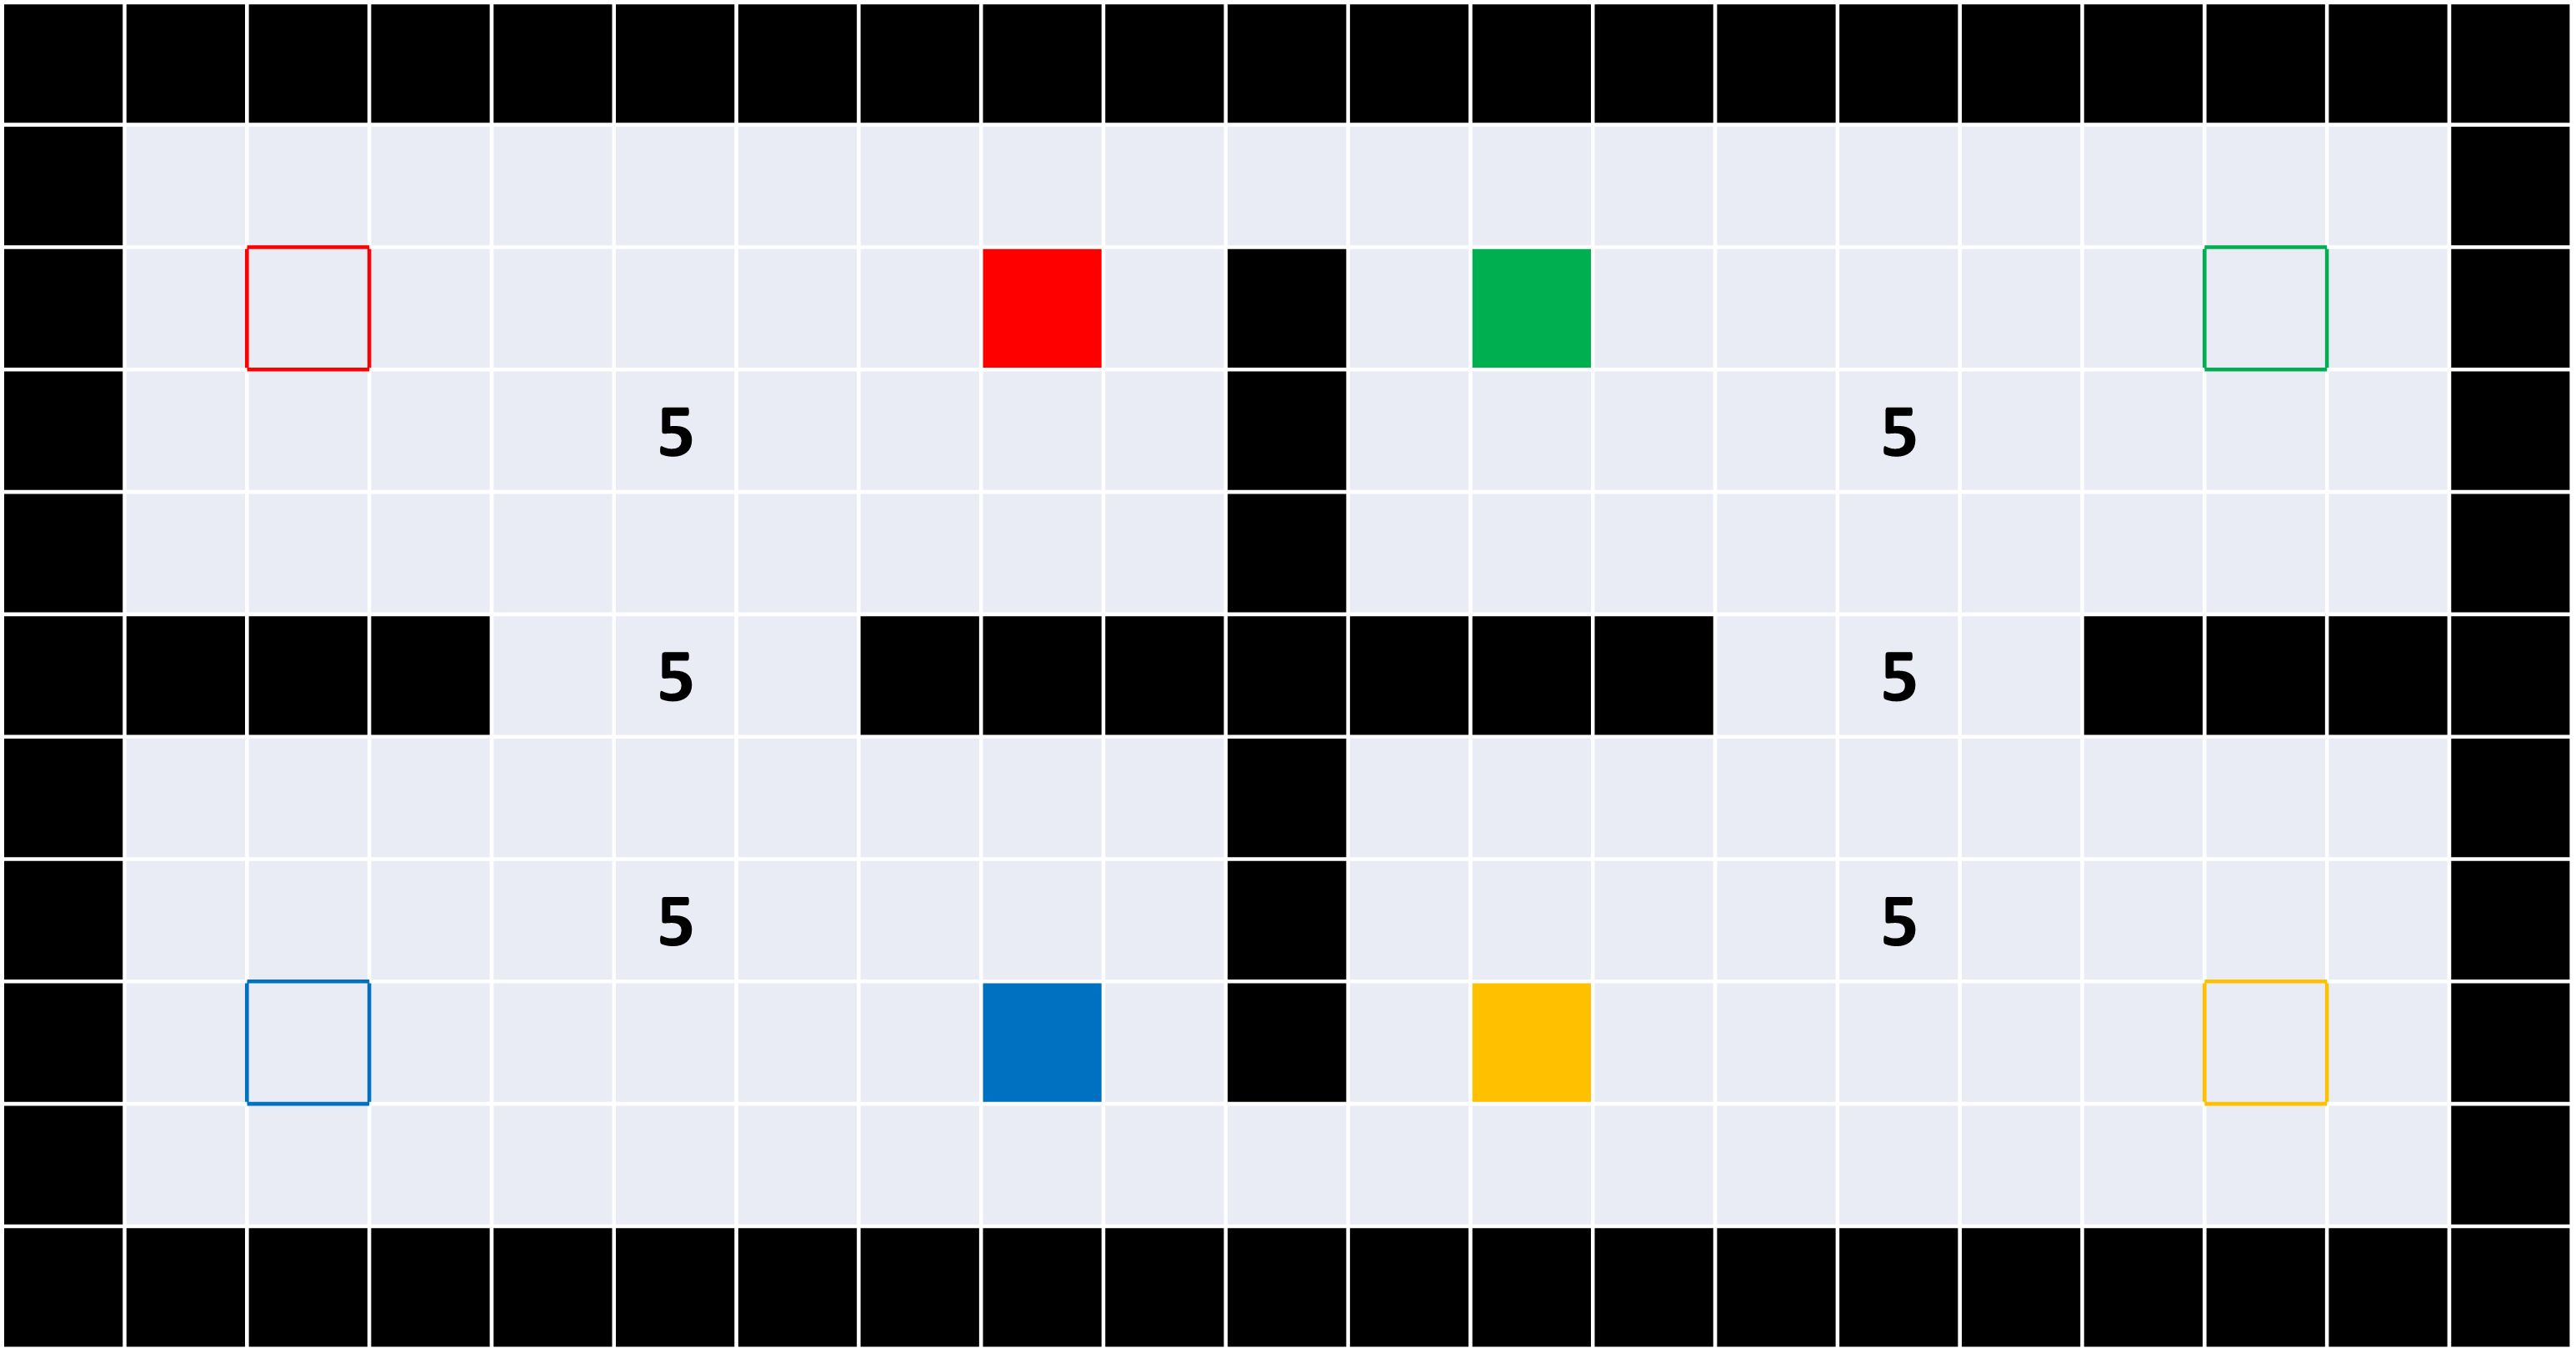
\includegraphics[width=0.27\textwidth]{Images/P2-4a.png}
%         \label{subfig:l3}} 
%     \caption{Grid SMAPF-PO benchmarks. Each color represents an agent. Initial positions are filled. Goal positions are bordered.}
%     \label{fig:multi-problems}
% \end{figure*}

% Figure~\ref{fig:multi-problems} visualizes all the Grids SMAPF-PO problems used in our experiments. Each color represents an agent. Initial positions are filled. Goal positions are bordered. 
% W are committed to make all these problems and our code publicly available. 

% \section{SMAPF-PO Results for Small Maps}



% \bibliography{ecai}
\end{document}
%%%%%%%%%%%%%%%%%%%%%%%%%%%%%%%%%%%%%%%%%%%%%%%%%%%%%%%%%%%%%%%%%%%%%%
